
\def\year{2021}\relax
% File: formatting-instruction.tex

\documentclass[letterpaper]{article} % DO NOT CHANGE THIS
\usepackage[margin=1in]{geometry}
% \usepackage{aaai21} % DO NOT CHANGE THIS
\usepackage{times} % DO NOT CHANGE THIS
\usepackage{helvet} % DO NOT CHANGE THIS
\usepackage{courier} % DO NOT CHANGE THIS
\usepackage[hyphens]{url} % DO NOT CHANGE THIS
\usepackage{graphicx} % DO NOT CHANGE THIS
\urlstyle{rm} % DO NOT CHANGE THIS
\def\UrlFont{\rm} % DO NOT CHANGE THIS
\usepackage{graphicx} % DO NOT CHANGE THIS
\usepackage{natbib} % DO NOT CHANGE THIS OR ADD OPTIONS
\usepackage{caption} % DO NOT CHANGE THIS OR ADD OPTIONS
\frenchspacing % DO NOT CHANGE THIS
\setlength{\pdfpagewidth}{8.5in} % DO NOT CHANGE THIS
\setlength{\pdfpageheight}{11in} % DO NOT CHANGE THIS

\usepackage{tikz}
	\usetikzlibrary{positioning,fit,calc, decorations, arrows, shapes, shapes.geometric}
	\usetikzlibrary{backgrounds}
	\usetikzlibrary{patterns}
	\usetikzlibrary{cd}
	
	\pgfdeclaredecoration{arrows}{draw}{
		\state{draw}[width=\pgfdecoratedinputsegmentlength]{%
			\path [every arrow subpath/.try] \pgfextra{%
				\pgfpathmoveto{\pgfpointdecoratedinputsegmentfirst}%
				\pgfpathlineto{\pgfpointdecoratedinputsegmentlast}%
			};
	}}
	%%%%%%%%%%%%
	\tikzset{AmpRep/.style={ampersand replacement=\&}}
	\tikzset{center base/.style={baseline={([yshift=-.8ex]current bounding box.center)}}}
	\tikzset{paperfig/.style={center base,scale=0.9, every node/.style={transform shape}}}

	\tikzset{is bn/.style={background rectangle/.style={fill=blue!35,opacity=0.3, rounded corners=5},show background rectangle}}
	% Node Stylings
	\tikzset{dpadded/.style={rounded corners=2, inner sep=0.7em, draw, outer sep=0.3em, fill={black!50}, fill opacity=0.08, text opacity=1}}
	\tikzset{dpad0/.style={outer sep=0.05em, inner sep=0.3em, draw=gray!75, rounded corners=4, fill=black!08, fill opacity=1}}
	\tikzset{dpad/.style args={#1}{every matrix/.append style={nodes={dpadded, #1}}}}
	\tikzset{light pad/.style={outer sep=0.2em, inner sep=0.5em, draw=gray!50}}
		
	\tikzset{arr/.style={draw, ->, thick, shorten <=3pt, shorten >=3pt}}
	\tikzset{arr0/.style={draw, ->, thick, shorten <=0pt, shorten >=0pt}}
	\tikzset{arr1/.style={draw, ->, thick, shorten <=1pt, shorten >=1pt}}
	\tikzset{arr2/.style={draw, ->, thick, shorten <=2pt, shorten >=2pt}}
	\tikzset{archain/.style args={#1}{arr, every arrow subpath/.style={draw,arr, #1}, decoration=arrows, decorate}}


	\tikzset{fgnode/.style={dpadded,inner sep=0.6em, circle},
	factor/.style={light pad, fill=black}}	
	
	
	\newcommand\cmergearr[4]{
		\draw[arr,-] (#1) -- (#4) -- (#2);
		\draw[arr, shorten <=0] (#4) -- (#3);
	}
	\newcommand\mergearr[3]{
		\coordinate (center-#1#2#3) at (barycentric cs:#1=1,#2=1,#3=1.2);
		\cmergearr{#1}{#2}{#3}{center-#1#2#3}
	}
	\newcommand\cunmergearr[4]{
		\draw[arr,-, , shorten >=0] (#1) -- (#4);
		\draw[arr, shorten <=0] (#4) -- (#2);
		\draw[arr, shorten <=0] (#4) -- (#3);
	}
	\newcommand\unmergearr[3]{
		\coordinate (center-#1#2#3) at (barycentric cs:#1=1.2,#2=1,#3=1);
		\cunmergearr{#1}{#2}{#3}{center-#1#2#3}
	}

	
	\usetikzlibrary{matrix}
	\tikzset{toprule/.style={%
	        execute at end cell={%
	            \draw [line cap=rect,#1] 
	            (\tikzmatrixname-\the\pgfmatrixcurrentrow-\the\pgfmatrixcurrentcolumn.north west) -- (\tikzmatrixname-\the\pgfmatrixcurrentrow-\the\pgfmatrixcurrentcolumn.north east);%
	        }
	    },
	    bottomrule/.style={%
	        execute at end cell={%
	            \draw [line cap=rect,#1] (\tikzmatrixname-\the\pgfmatrixcurrentrow-\the\pgfmatrixcurrentcolumn.south west) -- (\tikzmatrixname-\the\pgfmatrixcurrentrow-\the\pgfmatrixcurrentcolumn.south east);%
	        }
	    },
	    leftrule/.style={%
	        execute at end cell={%
	            \draw [line cap=rect,#1] (\tikzmatrixname-\the\pgfmatrixcurrentrow-\the\pgfmatrixcurrentcolumn.north west) -- (\tikzmatrixname-\the\pgfmatrixcurrentrow-\the\pgfmatrixcurrentcolumn.south west);%
	        }
	    },
	    rightrule/.style={%
	        execute at end cell={%
	            \draw [line cap=rect,#1] (\tikzmatrixname-\the\pgfmatrixcurrentrow-\the\pgfmatrixcurrentcolumn.north east) -- (\tikzmatrixname-\the\pgfmatrixcurrentrow-\the\pgfmatrixcurrentcolumn.south east);%
	        }
	    },
	    table with head/.style={
		    matrix of nodes,
		    row sep=-\pgflinewidth,
		    column sep=-\pgflinewidth,
		    nodes={rectangle,minimum width=2.5em, outer sep=0pt},
		    row 1/.style={toprule=thick, bottomrule},
  	    }
	}
\newif\ifprecompiledfigs
\precompiledfigsfalse
% \precompiledfigstrue

\newif\ifexternalizefigures\externalizefiguresfalse

\newif\ifappendix\appendixtrue
\newif\ifbody\bodyfalse

\ifexternalizefigures\else
	\usetikzlibrary{external}
	\tikzexternalize[prefix=tikz/]  % activate!
	% \usepackage{etoolbox}
	%  \AtBeginEnvironment{tikzcd}{\tikzexternaldisable} %... except careful of tikzcd...
	%  \AtEndEnvironment{tikzcd}{\tikzexternalenable}
\fi
%END_FOLD


%BEGIN_FOLD: Theorems and Tools

\usepackage{booktabs}       % professional-quality tables
\usepackage{amsfonts}       % blackboard math symbols
\usepackage{nicefrac}       % compact symbols for 1/2, etc.
\usepackage{microtype}      % microtypography
\usepackage{mathtools}		%also loads amsmath
\usepackage{amssymb, bbm}

%oli20: oops, this is vorboten :(
% \usepackage[format=plain,
%             labelfont={sl},
%             textfont={it,small}]{caption}

\usepackage{relsize}
\usepackage{environ} % http://ctan.org/pkg/environ; for capturing body as a parameter for idxmats

\usepackage{color}
%\usepackage{stmaryrd}

\usepackage{amsthm}
\usepackage{thmtools}

\theoremstyle{plain}
\newtheorem{theorem}{Theorem}[section]
\newtheorem{coro}{Corollary}[theorem]
\newtheorem{prop}[theorem]{Proposition}
\newtheorem{lemma}[theorem]{Lemma}
\newtheorem{fact}[theorem]{Fact}
\newtheorem{conj}[theorem]{Conjecture}

\theoremstyle{definition}

% no section numbers for theorems in AAAI style ... 
%joe17: can you reinstate this?
%oli20:done
\declaretheorem[name=Definition,qed=$\square$,numberwithin=section]{defn} %
\declaretheorem[name=Construction,qed=$\square$,sibling=defn]{constr}
\declaretheorem[qed=$\square$]{example}

\theoremstyle{remark}
\newtheorem*{remark}{Remark}

\usepackage{xstring}
\usepackage{enumitem}

\usepackage{environ}
\usepackage{xstring}

% Wow this works I'm brilliant
\def\wrapwith#1[#2;#3]{
	\expandarg\IfSubStr{#1}{,}{
		\expandafter#2{\expandarg\StrBefore{#1}{,}}
		\expandarg\StrBehind{#1}{,}[\tmp]
		\xdef\tmp{\expandafter\unexpanded\expandafter{\tmp}}
		#3
		\wrapwith{\tmp}[#2;{#3}]
	}{ \expandafter#2{#1} }
}
\def\hwrapcells#1[#2]{\wrapwith#1[#2;&]}
\def\vwrapcells#1[#2]{\wrapwith#1[#2;\\]}
\NewEnviron{mymathenv}{$\BODY$}

\newcommand{\smalltext}[1]{\text{\footnotesize#1}}
\newsavebox{\idxmatsavebox}
\def\makeinvisibleidxstyle#1#2{\phantom{\hbox{#1#2}}}
\newenvironment{idxmatphant}[4][\color{gray}\smalltext]{%
	\def\idxstyle{#1}
	\def\colitems{#3}
	\def\rowitems{#2}
	\def\phantitems{#4}
	\begin{lrbox}{\idxmatsavebox}$%$\begin{mymathenv}
	\begin{matrix}  \begin{matrix} \hwrapcells{\colitems}[\idxstyle]  \end{matrix}
		% &\vphantom{\idxstyle\colitems}
		\\[-0.05em]
		\left[
		\begin{matrix}
			\hwrapcells{\phantitems}[\expandafter\makeinvisibleidxstyle\idxstyle]  \\[-1.2em]
	}{
		\end{matrix}\right]		&\hspace{-0.8em}\begin{matrix*}[l] \vwrapcells{\rowitems}[\idxstyle] \end{matrix*}\hspace{0.1em}%
	\end{matrix}%
	$%\end{mymathenv}
	\end{lrbox}%
	\raisebox{0.75em}{\usebox\idxmatsavebox}
%	\vspace{-0.5em}
}

\newenvironment{idxmat}[3][\color{gray}\smalltext]
	{\begingroup\idxmatphant[#1]{#2}{#3}{#3}}
	{\endidxmatphant\endgroup}

\newenvironment{sqidxmat}[2][\color{gray}\smalltext]
	{\begingroup\idxmat[#1]{#2}{#2}}
	{\endidxmat\endgroup}


%%%%%%%%%%%%
% better alignment for cases
\makeatletter
\renewenvironment{cases}[1][l]{\matrix@check\cases\env@cases{#1}}{\endarray\right.}
\def\env@cases#1{%
	\let\@ifnextchar\new@ifnextchar
	\left\lbrace\def\arraystretch{1.2}%
	\array{@{}#1@{\quad}l@{}}}
\makeatother

\newcommand\numberthis{\addtocounter{equation}{1}\tag{\theequation}}

%oli20: apparently this is not allowed in AAAI style.
%oli21: but it helps me edit so I'm reenabling it until later
%oli25:
% \usepackage{xr}
% \usepackage{xr-hyper}
\usepackage{zref-xr}
% \usepackage{hyperref}
\zxrsetup{toltxlabel=true, tozreflabel=false}
\zexternaldocument*{pdg}
%oli24: the time has come... goodbye links and colors :(
% \usepackage{hyperref}
% \definecolor{deepgreen}{rgb}{0,0.5,0}
% \hypersetup{colorlinks=true, linkcolor=blue!50!black, urlcolor=magenta, citecolor=deepgreen}

\usepackage[noabbrev,nameinlink,capitalize]{cleveref}
\crefname{example}{Example}{Examples}
\crefname{defn}{Definition}{Definitions}
\crefname{prop}{Proposition}{Propositions}
\crefname{constr}{Construction}{Constructions}
\crefname{conj}{Conjecture}{Conjectures}
\crefname{fact}{Fact}{Facts}
%\crefname{section}{\S\!}{\S\!}


\usepackage{float}
% \usepackage{subcaption}
\newcounter{subfigure}
	% \captionsetup[subfigure]{subrefformat=simple,labelformat=simple}
	\renewcommand\thesubfigure{\thefigure(\alph{subfigure})}
    
\newenvironment{old}[1]{\par\noindent{\bf \Cref{#1}.} \em \noindent}{\par\medskip}

%% Version of recall that pulls the savebox:
% \usepackage{xpatch}
% \makeatletter
% \xpatchcmd{\thmt@restatable}% Edit \thmt@restatable
%    {\csname #2\@xa\endcsname\ifx\@nx#1\@nx\else[{#1}]\fi}% Replace this code
%    % {\ifthmt@thisistheone\csname #2\@xa\endcsname\typeout{oiii[#1;#2\@xa;#3;\csname thmt@stored@#3\endcsname]}\ifx\@nx#1\@nx\else[#1]\fi\else\csname #2\@xa\endcsname\fi}% with this code
%    {\ifthmt@thisistheone\csname #2\@xa\endcsname\ifx\@nx#1\@nx\else[{#1}]\fi
%    \else\fi}
%    {\typeout{oii Success1?}}{\typeout{oiii failure1?}} % execute code for success/failure instances
% \xpatchcmd{\thmt@restatable}% Edit \thmt@restatable
%    {\csname end#2\endcsname}
%    {\ifthmt@thisistheone\csname end#2\endcsname\else\fi}
%    {\typeout{oii Success2?}}{\typeout{oiii failure2?}}
% \newcommand{\recall}[1]{\medskip\par\noindent{\bf \expandarg\Cref{thmt@@#1}.} \begingroup\em \noindent
%    \expandafter\csname#1\endcsname* \endgroup\par\smallskip}
% \makeatother

\newcommand{\restate}[2]
	{\medskip\par\noindent{\bf \expandarg\Cref{thmt@@#1}.}%
 	\noindent\begingroup\em #2 \endgroup\par\smallskip}


%oli16: The extra space was because there was extra space in the paragraph, not
%because this length was too big. By breaking arrays, everything will be better.
\allowdisplaybreaks

\newcommand{\begthm}[3][]{\begin{#2}[{name=#1},restate=#3,label=#3]}

%TODO
\newcommand{\createversion}[2][{gray}{0.75}]{
	\definecolor{v#2color}#1\relax
    \expandafter\xdef\csname v#2on\endcsname{%
		% \xdef\gamma{\tau}%
		% \expandafter\renewcommand\csname v#2\endcsname{ONN}%
		% \expandafter\xdef{\csname v#2on\endcsname}##{{\color{v##2color} #1}}
	}
	\expandafter\xdef\csname v#2off\endcsname{
	% 	\expandafter\newcommand\csname v #2\endcsname[1]{{\color{v ##2 color} #1}}
	}
}
\createversion{test}
% \vteston
%END_FOLD

%BEGIN_FOLD   %%%% Version knobs %%%%%. 
%oli20: your commenting system is better than the one based on comment package, 
% which is way more problematic than I thought.
% I'm killing it and refactoring all comments to be like yours. I'm not annotating
% everything I'm doing here but the result will be way clearer and less problematic.

\definecolor{vfullcolor}{gray}{0.7}
\newcommand\vfull[1]{{\color{vfullcolor} #1}}
\renewcommand\vfull[1]{} % disable vfull

\definecolor{vleftoverscolor}{gray}{0.85}
\newcommand{\vleftovers}[1]{{\color{vleftoverscolor} #1}} 
\renewcommand{\vleftovers}[1]{} %disable vleftovers

\definecolor{notationcolor}{rgb}{0.9,0.9,.9} 
\newcommand{\notation}[1]{{\color{notationcolor} #1}}
\renewcommand{\notation}[1]{\ignorespaces} % disable notation

\definecolor{contentiouscolor}{rgb}{0.7,0.3,.1} 
\newcommand{\commentout}[1]{\ignorespaces} 

% \newcommand{\contentious}[1]{
% 	\noindent\colorbox{red!10!white}{\parbox{\linewidth-3pt}{\color{red!10!black}#1}}}
% \newcommand{\valpha}[1]{%
% 	% \colorbox{red!10!white}
% 	{\color{red!10!black}{#1}}%
% }
% \newcommand{\valpha}[1]{{\color{red!80!black}#1}}
\newcommand{\valpha}[1]{#1}

%END_FOLD


%BEGIN_FOLD definitions
%BEGIN_FOLD %%%%%   general shorthand I use   %%%%%%%%%%%%%%%%%

%\usepackage{stmaryrd}
%\DeclarePairedDelimiter{\ccbr}{\lBrace}{\rBrace}
%\DeclarePairedDelimiter{\bbr}{\llbracket}{\rrbracket}
%\DeclarePairedDelimiter{\ppr}{\llparenthesis}{\rrparenthesis}

\DeclarePairedDelimiterX{\bbr}[1]{[}{]}{\mspace{-3.5mu}\delimsize[#1\delimsize]\mspace{-3.5mu}}
\DeclarePairedDelimiter{\norm}{\lVert}{\rVert}

\let\Horig\H
\let\H\relax
\DeclareMathOperator{\H}{\mathrm{H}} % Entropy
\DeclareMathOperator{\I}{\mathrm{I}} % Information
\DeclareMathOperator*{\Ex}{\mathbb{E}} % Expectation
\DeclareMathOperator*{\argmin}{arg\;min}
\newcommand{\CI}{\mathrel{\perp\mspace{-10mu}\perp}} % Conditional Independence
\newcommand\mat[1]{\mathbf{#1}}
\DeclarePairedDelimiterX{\infdivx}[2]{(}{)}{%
	#1\;\delimsize\|\;#2%
}
\newcommand{\thickD}{I\mkern-8muD}
\newcommand{\kldiv}{\thickD\infdivx}


\newcommand{\todo}[1]{{\color{red}\ \!\Large\smash{\textbf{[}}{\normalsize\textsc{todo:} #1}\ \!\smash{\textbf{]}}}}
\newcommand{\note}[1]{{\color{blue}\ \!\Large\smash{\textbf{[}}{\normalsize\textsc{note:} #1}\ \!\smash{\textbf{]}}}}



% SPACES
\newcommand\Set{\mathbb{S}\mathrm{et}}
\newcommand\FinSet{\mathbb{F}\mathrm{in}\mathrm{S}\mathrm{et}}
\newcommand\Meas{\mathbb{M}\mathrm{eas}}
\newcommand\two{\mathbbm 2}

%END_FOLD

%BEGIN_FOLD %%%%%    PDG-specific macros     %%%%%%%%%%%%%%%%
\DeclarePairedDelimiterXPP{\SD}[1]{}{[}{]}{_{\text{sd}}}{\mspace{-3.5mu}\delimsize[#1\delimsize]\mspace{-3.5mu}}
		
%\usepackage{stmaryrd}
%\newcommand{\none}{\varobslash}
\newcommand{\none}{\bullet}

\def\sheq{\!=\!}
\DeclareMathOperator\dcap{\mathop{\dot\cap}}
\newcommand{\tto}{\rightarrow\mathrel{\mspace{-15mu}}\rightarrow}

\newcommand{\bp}[1][L]{\mat{p}_{\!_{#1}\!}}
\newcommand{\V}{\mathcal V}
\newcommand{\N}{\mathcal N}
\newcommand{\Ed}{\mathcal E}
\newcommand{\pdgvars}[1][]{(\N#1, \Ed#1, \V#1, \mat p#1, \beta#1)}


\DeclareMathAlphabet{\mathdcal}{U}{dutchcal}{m}{n}
\DeclareMathAlphabet{\mathbdcal}{U}{dutchcal}{b}{n}
%joe1:out of curiousity, why not use \mathcal?  That's what you use
%for BNs.  Why do PDG use a different font?
\newcommand{\dg}[1]{\mathbdcal{#1}}
\newcommand{\var}[1]{\mathsf{#1}}
\newcommand\Pa{\mathbf{Pa}}

%oli20: better spacing
% \newcommand{\IDef}[1]{\mathit{IDef}_{#1}}
\newcommand{\IDef}[1]{\mathit{IDef}_{\!#1}}

\newcommand\Inc{\mathit{Inc}}
\newcommand{\PDGof}[1]{{\dg M}_{#1}}
%oli22: a macro for unweighted PDGs
\newcommand{\UPDGof}[1]{{\dg N}_{#1}}
\newcommand{\WFGof}[1]{\Psi_{{#1}}}
%oli22: and for unweighted ones
\newcommand{\FGof}[1]{\Phi_{{#1}}}
%oli22: want to refer to the variable graph
\newcommand{\Gr}{\mathcal G}
%oli22: Gibbs Free Energy conflicts with \mathcal G. Now it lives in 
% this macro.
\newcommand\GFE{\mathit{G\mkern-4mu F\mkern-4.5mu E}}
%oli22: Right now we're using (\N, \V) to refer to variables of a
% PDG. I think it's important to keep both \N and \V but am happy to change
% the way we combine them. Factored into a macro so it's easier to change.
\newcommand{\varsNV}[1][\N,\V]{(#1)}


% \makeatletter %Arguments: L, X, Y, \scriptscriptstyle, -1pt (for raisebox)
% \newcommand{\ed@helper}[5]{#2\!%
%   \overset{\smash{\mskip-5mu\raisebox{-1pt}{$\scriptscriptstyle
%         #1$}}}{\rightarrow}\! #3} 
% \makeatother

%oli22: the edge notation is now uniform. Choose between the following
% Default: display as "X -L-> Y" (leave uncommented).
\newcommand{\ed}[3]{#2\!%
  \overset{\smash{\mskip-5mu\raisebox{-1pt}{$\scriptscriptstyle
        #1$}}}{\rightarrow}\! #3} 
% Option: uncomment to display as  "L = (X,Y,\ell)" instead.
% \renewcommand{\ed}[3]{#2 = (#1,#3,\ell)} 
\newcommand{\alle}[1][L]{_{ \ed {#1}XY}}


\begin{document}
\appendix
\onecolumn
%\section{Proofs} \label{sec:proofs}
%oli10: added this subsection and reorganized propositions /
%definitions accordingly.i
	%joe9: removed section
%	\subsection{Standard Definitions and General Facts}
%joe9: let's be consistent and write \mu for the default distribution
%	For brevity, we use the standard notation and write $p(x, y)$
%        instead of $p(X \!=\! x, Y \!=\! y)$, $p(x \mid y)$ instead of
	%        $p(X \!=\! x\mid Y \!=\! y)$, and so forth.
		For brevity, we use the standard notation and write $\mu(x, y)$
	instead of $\mu(X \!=\! x, Y \!=\! y)$, $\mu(x \mid y)$ instead of
	$\mu(X \!=\! x\mid Y \!=\! y)$, and so forth.
%joe9: I don't understand this
%        So long as $x$ is bound solely as an element of $\V(X)$, the
%        meaning is unambiguous.  

	%joe9: this should go where we use it; I put it there
	\commentout{
\begin{defn}[Conditional Entropy]
	If $p$ is a distribution over a set $\Omega$ of out comes, and $X$ and $Y$ are random variables on $\Omega$, then the \emph{conditional entropy}, $\H_p(X \mid Y)$, is defined as 

\end{defn}

%joe9*: I think we shoul cut this; we don't need it.
	\begin{defn}[Sets as Variables] \label{def:set-rv}
	Sets of random variables as random variables. If $S$ is a set of random variables $X_i : \Omega \to \V(X_i)$ on the same set of outcomes $\Omega$, we consider $S$ itself to be the random variable taking values $\V(X) = \{(x_1, \ldots, x_i \ldots) \}$ for $x_i \in \V(X_i)$. Formally, we define its value on a world $\omega$ to be $S(\omega) := (X_1(\omega), \ldots, X_i(\omega), \ldots)$. 
\end{defn}

%joe9*: I think we should cut this; we don't need it.  We need strict
%convexity, which has a much simpler definition.                
%oli10: added
\begin{defn}[Strong Convexity] \label{def:strong-convexity}
	A real-valued function is $m$-\emph{strongly convex}, if there is a quadratic lower bound, with coefficient $m$, away from its first order approximation. More precisely, it is $m$ strongly convex if for every $x, y$ in its domain, 
	\[ f(y) \geq f(x) + \Big\langle\nabla f(x), y-x \Big\rangle + m\norm{x-y}^2_2 \]
\end{defn}

%joe9*: we should cut this; it's doubtless a standard reslt, and we
%don't need it.
%oli11: I actually asked Bobby for a reference and he said it was so
%standard that everyone just says it. He even looked through a couple
%standard convex analysis books and says it's not there. I proved it
%because you asked for a result I couldn't find one. 
%oli11: It may be worth keeping some of the strong convexity stuff
%around though; strong convexity is a _lot_ more useful for finding
%the minimum than strict convexity, and ML people will immediately
	%know that this means it is efficient.
%joe10: NO!  Don't clutter up the paper with things ou don't need!
	%This is bad style!
\begin{prop}\label{prop:neg-ent-convex}
%joe8*: you can't pull 1-strong convexity out of a hat, and define it
%in the proof.  You need to define it, and explain why you care.  Your
%proof also looks at hte function xlog x, so whynot state the
%proposition in terms of that?
%oli10: definition added above
  Negative entropy, restricted to a finite probability
			simplex, is 1-strongly convex. 
\end{prop}
\begin{proof}
	%https://math.stackexchange.com/questions/3077287/how-to-show-negative-entropy-function-fx-x-logx-is-strongly-convex
	Let $X$ be a finite set; the function $f: \Delta(X) \to \mathbb R$ given by $\vec x \mapsto \sum x_i \log x_i$ is strongly convex, as 
	\begin{equation*}
		\partial_j f(\vec x) =  \partial_j\left[\sum_i x_i \log x_i \right] = 
			x_j \partial_j \big[\log x_j \big] + \log x_j = 1 + \log x_j
	\end{equation*}
	So
	\begin{align*}
		\Big\langle \nabla f(x) - \nabla f(y),~ x-y\Big\rangle 
			&= \sum_i \Big((\partial_i f)(\vec x) - (\partial_i f)(\vec y)\Big)(x_i - y_i) \\
			&= \sum_i \Big(\log x_i  - \log y_i \Big)(x_i - y_i) \\
			% &= \sum_i x_i \log x_i + y_i \log y_i + 2 
		\intertext{As $\log$ is concave, we have $\log(y_i) \leq \log(x_i) + (y_i-x_i) \frac{\mathrm d}{\mathrm d x_i} [\log(x_i)]$, and so $\log x_i - \log y_i \geq (1/x) (x - y)  \geq (x-y)$, we have}
		\Big\langle \nabla f(x) - \nabla f(y),~ x-y\Big\rangle
			&= \sum_i \Big(\log x_i  - \log y_i \Big)(x_i - y_i) \\ % from above
			&\geq \sum_i (x_i-y_i)^2 \cdot \frac1{x_i}\\
			&\geq \sum_i (x_i-y_i)^2 \\
			&= \norm{x-y}^2_2 \numberthis\label{proofeqn:strong1}
%joe9: When I latex this, I get the error ``You can't use `\halign' in
%math mode.''  (I've gotten this error all along; it's nothing new.) 
%oli11*: only in aligns that have a \numberthis, or all align environments?
% we should fix this...
%joe10: I'm not sure; I didn't check.  I shouldn't have to spend time
%doing thi!
	\end{align*}
	At the same time, the condition for convexity can be phrased in terms of gradients as the condition that for all $x,y$,
	\[  \Big\langle \nabla f(x) - \nabla f(y),~ x-y\Big\rangle \geq 0\]
	So together with \eqref{proofeqn:strong1}, we conclude that the function $f - \norm{x-y}^2_2$ is convex. Therefore, $f$ is 1-strongly convex.
\end{proof}

	}
%joe9: \end{commentout}
	
\subsection{Properties of Scoring Semantics}


	\begin{vfull}
	\thmsetconvex*
	\begin{proof}
		Choose any two distributions $p, q \in \SD{M}$ consistent with $M$, any mixture coefficient $\alpha \in [0,1]$, and any edge $(A,B) \in \Ed$.
		
		By the definition of $\SD{M}$, we have $p(B = b \mid A = a) = q(B = b \mid A = a) = \mat p_{A,B}(a,b)$.  
		For brevity, we will use little letters ($a$) in place of events ($A = a$).
		Therefore, $p(a\land b) = \mat p_{A,B}(a,b) p(a)$ and $q(ab) = \mat p_{A,B}(a,b) q(a)$. Some algebra reveals:
		\begin{align*}
			\Big( \alpha p + (1-\alpha) q \Big) (B = b \mid A = a) &= 
			\frac{\Big( \alpha p + (1-\alpha) q \Big) (b \land a)}{\Big( \alpha p + (1-\alpha) q \Big) (a)} \\
			&= \frac{ \alpha p(b \land a) + (1-\alpha) q(b \land a) }{\Big( \alpha p(a) + (1-\alpha) q (a)} \\
			&= \frac{ \alpha \mat p_{A,B}(a,b) p(a) + (1-\alpha) \mat p_{A,B}(a,b) q(a) }{\Big( \alpha p(a) + (1-\alpha) q (a)} \\
			&=\mat p_{A,B}(a,b) \left(\frac{ \alpha  p(a) + (1-\alpha) q(a) }{\Big( \alpha p(a) + (1-\alpha) q (a)}\right)\\
			&= \mat p_{A,B}(a,b)
		\end{align*}
		and so the mixture $\Big(\alpha p + (1-\alpha) q \Big)$ is also contained in $\SD{M}$.
	\end{proof}
\end{vfull}
%joe9: just because it's n appendix, it doesn't mean that we shouldn't
%tell a story.
In this section, we prove the properties of scoring functions that we
mentioned in the main text,
Propositions~\ref{prop:sd-is-zeroset}, \ref{prop:sem3}, and
\ref{prop:consist}.  We repeat the statements for the reader's convenience.

%joe9: put this first
%	\begin{prop}\label{prop:sd-is-zeroset}
%oli15: consistency
% \begin{old}{prop:sd-is-zeroset}
% 	For any PDG $\dg M$, $\SD{\dg M} = \{ \mu : \bbr{\dg M}_0(\mu) = 0\}$. 
% \end{old}
\recall{prop:sd-is-zeroset}
\begin{proof}
	 By taking $\gamma = 0$, the score is just $\Inc$. By
%joe9
%                 definition, any $\mu \in \SD{\dg M}$ satisfies all
%                 constraints, hence satisfies $\mu(Y \mid X=x) =
%                 \bp(x)$ for any $L \in \Ed^{\dg M}$ and $x$ with
%                 \bp(x)$ for any $L \in \Ed^{\dg M}$ and $x$ with
			 definition, a distribution $\mu \in \SD{\dg M}$ satisfies
	  all the
			 constraints, so $\mu(Y = \cdot \mid X=x) =
			 \bp(x)$ for all edges $X \rightarrow Y \in \Ed^{\dg
			   M}$ and $x$ with 
%joe9*: this needs a reference
%oli11
			 % $\mu(X=x)>0$. By Gibbs inequality,
			 $\mu(X=x)>0$. By Gibbs inequality
			 \cite{mackay2003information}, 
			 $\kldiv{\mu(Y|x)}{\bp(x)} = 0$. Since this is true
			 for all edges, we must have $\Inc_{\dg M}( \mu) =
			 0$. Conversely, if $\mu \notin \SD{\dg M}$, then it
			 fails to marginalize to the cpd $\bp$ on some edge
%joe9
			 %                 $L$, and so again by Gibbs inequality
							  $L$, and so again by Gibbs inequality,
			 $\kldiv{\mu(Y|x)}{\bp(x)} > 0$. As relative entropy
			 is non-negative, the sum of these terms over all
			 edges must be positive as well, and so $\Inc_{\dg M}(
			 \mu) \neq 0$. %This is true whether or not $\dg M$ is
						   %consistent. 
\end{proof}


%joe9
Before proving the remaining results, we prove a lemma that will be useful
in other contexts as well. 

%oli11: aaahhh it took me an hour to edit this, and I don't think
%anything even changed. 
% Why did you modify it? It was so much cleaner before.
%joe10: I thought it was overkill ... 
\begin{lemma}
	% [name=\Cref{prop:convex} analog, 	restate=thmincconvex]
	\label{thm:inc-convex}
	$\Inc_{\dg M}( \mu)$ is a convex function of $\mu$.
\end{lemma}
\begin{proof}
	It is well-known that $\thickD$ is convex, in the sense that 
	\[ \kldiv{\lambda q_1 + (1-\lambda) q_2 }{ \lambda p_1
			  + (1-\lambda) p_2} \leq \lambda \kldiv {q_1}{ p_1} +
%joe9
			%                (1-\lambda) \kldiv{q_2}{p_2} \]
							(1-\lambda) \kldiv{q_2}{p_2}. \] 
%joe9
%		Choose any edge $L \in \Ed$ from $A$ to $B$, and also
			%                any $a \in \mathcal V(A)$.
Given an edge $L \in \Ed$ from $A$ to $B$ and $a \in \mathcal V(A)$,
and   
%oli11
% etting $q_1 = q_2 = \bp(a)$, we get that
setting $q_1 = q_2 = \bp(a)$, we get that
	\[ \thickD(\bp(a) \ ||\ \lambda p_1 + (1-\lambda) p_2)
			\leq \lambda \thickD (\bp(a) \ ||\ p_1) + (1-\lambda)
%joe9
			%                \thickD(\bp(a)\ ||\ p_2) \]
							\thickD(\bp(a)\ ||\ p_2). \] 
	Since this is true for every $a$ and edge, we can take
		   a weighted sum of these inequalities for each $a$
%joe9
		   %               weighted by $p(A=a)$, and therefore
						  %		\begin{align*}
		   weighted by $p(A=a)$; thus, 
%oli11: I think the NeurIPS style guide wants us to avoid
% the TeX primitive $$, in favor of \[, as this behavior can be styled, while the TeX primitve cannot. 
%oli11: I also find this a lot uglier than the \align*. 
	\begin{align*}
		% \E_{a\sim p(A=a)} \kldiv{\bp(a)}{\lambda p_1 + (1-\lambda) p_2} &\leq \E_{a\sim p(A=a)}\lambda \kldiv {\bp(a)}{p_1} + (1-\lambda) \thickD(\bp(a)\ ||\ p_2)
%oli11: wrong notation for maringal on A. Others changed inline.
		% \E_{a\sim p} \kldiv{\bp(a)}{\lambda p_1 +
		\E_{a\sim p_A} \kldiv{\bp(a)}{\lambda p_1 +
%oli11: add alignment. Ohers also, but not marked.
			% (1-\lambda) p_2} \leq \E_{a\sim
			(1-\lambda) p_2} &\leq 
			 \E_{a\sim p_A}\lambda \kldiv {\bp(a)}{p_1} +
%joe9
					%                        (1-\lambda) \thickD(\bp(a)\ ||\ p_2) \\
											(1-\lambda)
%oli11
					% \thickD(\bp(a)\ ||\ p_2)$$ and $$
					 \kldiv{\bp(a)}{p_2} \\
%oli11: the next line does what you added; I'm adding more
% \intertext{and}
\intertext{and so taking a sum over all edges, }
					\sum_{(A, B) \in \Ed}\mskip-10mu\E_{a\sim p_A} \kldiv{\bp(a) }{\lambda p_1 + (1-\lambda) p_2} 
			&\leq \sum_{(A, B) \in
							  \Ed}\mskip-10mu\E_{a\sim p_A}\lambda
							\kldiv{\bp(a)}{p_1} + (1-\lambda)
							\kldiv{\bp(a)}{p_2} \\
		%joe9
%oli11: reinstated intertext and deleted ``$$ and $$''
%oli11 removing "and so" breaks flow of equantions; replace with \implies
		% \intertext{and so,}
	\implies\qquad
		\Inc_{\dg M}( \lambda p_1) + (1-\lambda)p_2)
%joe9
%                        &\leq \lambda \Inc_{\dg M}(p_1) + (1-\lambda)
					%                        \Inc}{\dg M}(p_2)
%oli11: inserted missing alignment character
					&\leq \lambda \Inc_{\dg M}(p_1) + (1-\lambda)
					\Inc_{\dg M}(p_2). 
											%joe9
				\end{align*}
%		Therefore $\Inc_{\dg M}( \mu)$ is a convex function of $\mu$
%oli11:
% I'm still not sure why you even re-structured the TeX of this proof, but it confused my editor. 
	Therefore, $\Inc_{\dg M}( \mu)$ is a convex function of $\mu$.
\end{proof}

%joe9: added glue
The next proposition gives us a useful representation of $\bbr{M}_\gamma$.
\recall{prop:nice-score}
% \endold
% \propnicescore*
\begin{proof}
  \begin{align*}
		\bbr{\dg M}_\gamma(\mu) &:= \Inc_{\dg M}( \mu) + \gamma \IDef{\dg M}(\mu) \\
			% Next, replace expressions for Inc and Extra
			&= \left[\sum\alle \beta_L \E_{x\sim \mu_X}\kldiv[\Big]{ \mu(Y | X \sheq x) }{\bp(x) } \right]  + \gamma \left[\sum\alle \H_\mu(Y\mid X) ~-\H(\mu)\right]\\
			% Combine the summations and expectations
			&= \sum\alle 
				\E_{x \sim \mu_{\!_X}}  \left[ \beta_L\; \kldiv[\Big]{ \mu(Y \mid x) }{\bp(Y \mid x) } + \gamma \; \H(Y \mid X\sheq x) \right]  - \gamma \H(\mu) \\ 
			% Now, Expand relative and conditional entropy
			&= \sum\alle 
				\E_{x \sim \mu_{\!_X}}  \left[ \beta_L\; \left(\sum_{y \in \V(Y)} \mu(y \mid x) \log\frac{\mu(y\mid x)}{\bp(y\mid x)}\right) + \gamma \; \left(\sum_{y \in \V(Y)} \mu(y\mid x) \log \frac{1}{\mu(y\mid x)} \right) \right]  - \gamma  \H(\mu) \\ 
			%combine common \sum \mu(y | x) 
			&= \sum\alle 
				\E_{x \sim \mu_{\!_X}}  \left[ \sum_{y \in \V(Y)} \mu(y \mid x) \left(  \beta_L\; \log\frac{\mu(y\mid x)}{\bp(y\mid x)} + \gamma \; \log \frac{1}{\mu(y\mid x)} \right) \right]  - \gamma  \H(\mu) \\
			% Expand entropy and reduce sum to expectation
			&= \sum\alle 
				\E_{x \sim \mu_{\!_X}}  \left[ \E_{y \sim \mu(Y \mid X=x)} \left(  \beta_L\; \log\frac{\mu(y\mid x)}{\bp(y\mid x)} + \gamma \; \log \frac{1}{\mu(y\mid x)} \right) \right]  - \gamma \sum_{\mat w \in \V(\dg M)} \mu(\mat w) \log \frac{1}{\mu(\mat w)} \\  
			% combine expectation.
			&= \sum\alle 
				\E_{x,y \sim \mu_{\!_{XY}}}  \left[ \beta_L\; \log\frac{\mu(y\mid x)}{\bp(y\mid x)} + \gamma \; \log \frac{1}{\mu(y\mid x)}  \right]  - \gamma  \E_{\mat w \sim \mu} \left[ \log \frac{1}{\mu(\mat w)}\right] \\
			% swap sum and expectation, and use log rule to split kl divergence
			&= \E_{\mat w \sim \mu} \Bigg\{   \sum_{ X \xrightarrow{\!\!L} Y  } \left[
				\beta_L \log \frac{1}{\bp(y\mid x)}   - \beta_L  \log \frac{1}{\mu(y \mid x)}+ \gamma \log \frac{1}{\mu(y \mid x)} \right]\Bigg\}  -  \gamma  \E_{\mat w \sim \mu} \left[\log \frac{1}{\mu(\mat w)}\right] \\
			% combine
			&=  \E_{\mat w \sim \mu} \Bigg\{ \sum_{ X \xrightarrow{\!\!L} Y  } \left[
				\beta_L \log \frac{1}{\bp(y\mid x)} + (\gamma - \beta_L ) \log \frac{1}{\mu(y \mid x)} \right] - \gamma \log \frac{1}{\mu(\mat w)} \Bigg\} 
	\end{align*}
\end{proof}

	%joe9
%        	\begin{prop} \label{prop:convex-if-gamma-small}
%	  For a PDG $\dg M$, and any $\gamma$ such that $0 <
%          \gamma \leq \min_L \beta_L^{\dg M}$, then $\bbr{\dg
%          If $\dg M$ is a PDG and   $0 < \gamma < \min_L \beta_L^{\dg M}$, then
%          then $\bbr{\dg
%                  M}_\gamma$ is a strictly convex function of $\mu$.
%	\end{prop}
We can now prove         Proposition~\ref{prop:sem3}.
% \begin{old}{prop:sem3}
% If $\dg M$ is a PDG and
% $0 < \gamma
% \leq \min_L \beta_L^{\dg M}$, then
% $\bbr{\dg M}_\gamma^*$ is a singleton.
% \end{old}
\recall{prop:sem3}
\begin{proof}
	  %joe9:
It suffices to show that $\bbr{\dg
			  M}_\gamma$ is a strictly convex function of $\mu$,
since every strictly convex function has a unique minimum.
%joe9
%We can rewrite the semantics as
Note that
	\begin{align*}
		\bbr{M}_\gamma(\mu) 
			&= \E_{\mat w \sim \mu} \Bigg\{   \sum_{ X \xrightarrow{\!\!L} Y  } \left[
				\beta_L \log \frac{1}{\bp(y\mid x)} + (\gamma - \beta_L ) \log \frac{1}{\mu(y \mid x)} \right] - \gamma \log \frac{1}{\mu(\mat w)} \Bigg\} \\
			&= \E_{\mat w \sim \mu} \Bigg\{   \sum_{ X \xrightarrow{\!\!L} Y  } \left[ \gamma \log \frac{1}{\bp(y\mid x)} + 
				(\beta_L - \gamma) \log \frac{1}{\bp(y\mid x)} - (\beta_L -\gamma) \log \frac{1}{\mu(y \mid x)} \right] - \gamma \log \frac{1}{\mu(\mat w)} \Bigg\}  \\
			&= \E_{\mat w \sim \mu} \Bigg\{   \sum_{ X \xrightarrow{\!\!L} Y  } \left[ \gamma \log \frac{1}{\bp(y\mid x)} + 
				(\beta_L - \gamma) \log \frac{\mu(y\mid x)}{\bp(y\mid x)} \right] - \gamma \log \frac{1}{\mu(\mat w)} \Bigg\} \\
			&=  \sum_{ X \xrightarrow{\!\!L} Y  } \left[ \gamma \E_{x,y \sim \mu_{\!_{XY}}} \left[\log \frac{1}{\bp(y\mid x)} \right] + 
				(\beta_L - \gamma) \E_{x\sim\mu_X} \kldiv[\Big]{\mu(Y\mid x)}{\bp( x)} \right] - \gamma \H(\mu)
	\end{align*}
	The first term, 
	\( \E_{x,y \sim \mu_{\!_{XY}}} \left[-\log {\bp(y\mid x)}\right] \) 
	is linear in $\mu$, as $\bp(y\mid x)$ does not depend on $\mu$. %joe9: you need a reference here.  
As for the second term, it is well-known that KL divergence is convex, in the sense that 
	\[ \kldiv{\lambda q_1 + (1-\lambda) q_2 }{ \lambda p_1 + (1-\lambda) p_2} \leq \lambda \kldiv {q_1}{ p_1} + (1-\lambda) \kldiv{q_2}{p_2} \]
	Therefore, for a distribution on $Y$, setting $p_1 =
%joe9
%                p_2 = \bp(x)$, we discover that for any two
%               conditional marginals $\mu_1(Y \mid X=x)$ and
			%                $\mu_2(Y\mid X=x)$,that
 p_2 = \bp(x)$, for all conditional marginals $\mu_1(Y \mid X=x)$ and
			$\mu_2(Y\mid X=x)$,
	\[ \kldiv{\lambda \mu_1(Y\mid x) + (1-\lambda)
			  \mu_2(Y\mid x) }{ \bp(x) } \leq \lambda \kldiv
			   {\mu_1(Y\mid x)}{\bp(x)} + (1-\lambda)
%joe9
			   %                   \kldiv{\mu_2(Y\mid x)}{\bp(x)} \]
								  \kldiv{\mu_2(Y\mid x)}{\bp(x)}. \] 
	So $\kldiv*{\mu(Y\mid x)}{\bp( x)}$ is convex. As
			convex combinations of convex functions are convex,
			the second term, $\E_{x\sim\mu_X}\kldiv*{\mu(Y\mid
			  x)}{\bp( x)}$, is convex.
%joe9: we need a reference
%                Finally, negative entorpy is 1-strongly convex, by
			%                (\Cref{prop:neg-ent-convex}).
Finally, negative entropy is well known to be strictly convex.                

%joe10: what is this adding
%By addition and scaling of the convexity inequalities, any
			Any non-negative linear combinations of the three
			terms is convex, and if this combination applies a
%joe9
%                positive coefficient $\gamma$ to the negative entropy,
%                it must be $\gamma$-strongly convex. Therefore, so
%                long as $(\beta_L \geq \gamma)$ for every $L \in
			positive coefficient to the (strictly convex) negative entropy,
			it must be strictly convex. Therefore, as
			long as $\beta_L \geq \gamma$ for all edges $L \in
			\Ed^{\dg M}$, $\bbr{\dg M}_\gamma$ is
%joe9
%                $\gamma$-strongly convex, and in particular, strictly
strictly convex.  The result follows.
\end{proof}


%oli12: Factor out joint argument; otherwise
%  3.3 and 3.4 have a circular dependence or duplicate each other.
%oli12: 
% It seems we also you had a few subtle bugs and things that caused me to 
% totally re-evaluate whether my proof was correct. It is, and I've fixed up
% yours to be correct as well. I wish I hadn't spent 3 additional hours on this.
We first prove a more general version of \Cref{prop:consist}.
\begin{lemma}\label{lem:gamma2zero}
$\lim\limits_{\gamma\to0}\bbr{\dg M}_\gamma^* \subseteq \bbr{\dg M}_0^*$ 
%where $\Inc(\dg M) := \min_{\mu} \Inc_{\dg M}(\mu)$.
\end{lemma}
\begin{proof}
\def\lb{k}
\def\ub{K}  
%oli12: ... it turns out you maybe can't do it this way? 
% continuity seems too weak.
%oli12 generalizing your proof.
% Suppose that $\bbr{\dg M}^* = \{\mu^*\}$ and 
% that $\bbr{\dg M}^*_\gamma = 
% \{\mu_\gamma\}$.  By the argument above, $\mu_\gamma \rightarrow
% \mu^*$.
% Choose any $\mu^* \in \lim_{\gamma\to0}\bbr{\dg M}^*_\gamma$. By the definition 
% of this limit, we must have a sequence $(\gamma_i, \mu_i)$ such that $\gamma_i\to0$ 
% and $\mu_i\to\mu^*$, with each $\mu_i \in \bbr{\dg M}^*_{\gamma_i}$.
% %
% Since $\bbr{\dg M }_\gamma$ is clearly continuous as a function of
% $\gamma$, it follows that $\bbr{\dg M}_\gamma  (\mu_\gamma)
% \rightarrow \bbr{\dg M}_0(\mu^*)$.  

Since $\IDef{\dg M}$ is a finite sum of entropies
and conditional entropies over the variables $\N^{\dg M}$, which have finite support%
%oli12: removed
%  ; thus
, it is bounded.
Thus, there exist bounds $k$ and $K$ depending only on $\N^{\dg M}$ and
$\V^{\dg M}$, such that $\lb \leq \IDef{\dg M}(\mu) \leq \ub$ for all $\mu$.
%
%oli12: added reasoning
Since $\bbr{\dg M}_\gamma = \Inc_{\dg M} + \gamma \IDef{\dg M}$,
it follows that, for all $\mu \in \V(\dg M)$, we have
%oli12: change to display mode
\[ \Inc_{\dg M}( \mu) + \gamma\lb \leq~ \bbr{\dg M }_\gamma(\mu) 
\leq~  \Inc_{\dg M}( \mu) + \gamma\ub. \]
%joe10: added instead
%oli12: This bit is garbled; the antecedents are all wrong, as "this minimum"
%must refer to [[M]], not Inc, and it's also not clear why "the minimum is
%achieved" results in the particular sequence \mu_gamma that you had before....
%I rewrote it more carefully.
%oli12: This next bit is actually tricky. slowing down.
For any fixed $\gamma$, since this inequality holds for all $\mu$, and both $\Inc$ and $\IDef{}$ are bounded below, it must be true that 
\[
\min_{\mu \in \Delta\V(\dg M)} \Big[ \Inc_{\dg M}( \mu) + \gamma\lb \Big]
~\leq~ \min_{\mu \in \Delta\V(\dg M)}\bbr{\dg M }_\gamma(\mu) ~\leq~  \min_{\mu \in \Delta\V(\dg M)} \Big[ \Inc_{\dg M}( \mu) + \gamma\ub \Big]. \]
even though the distributions that minimize each expression will in general be different.
Let $\Inc(\dg M) = \min_{\mu} \Inc_{\dg M}(\mu)$.
Since $\Delta\V(\dg M)$ is compact, this minimum of the middle term is achieved. 
Therefore, for any $\mu_\gamma \in \bbr{\dg M}^*_\gamma(\mu)$ that minimizes it, we have
%oli12: a little ambiguous about which minimum we're taking... removed.
% Taking the minimum over $\Delta\V(\dg M)$, we get that
$$\Inc(\dg M) +\gamma \lb \le \bbr{\dg M }_\gamma(\mu_\gamma) \le
		 \Inc(\dg M) +\gamma \ub$$ for all $\gamma \ge 0.$
% $$\Inc(\dg M) +\gamma \lb \le \bbr{\dg M }_\gamma(\mu_\gamma) \le$$
Now taking the limit as $\gamma\rightarrow 0$ from above, we get that
$\Inc(\dg M) = \bbr{\dg M }_0(\mu^*)$.
%joe10* You missed the punchline, which I just added
Thus, $\mu^* \in \bbr{\dg M}_0^*$, as desired.
\commentout{

		\begin{alignat*}{4}\relax
			&\forall\gamma,\mu.~&\gamma\lb &~\leq~& \gamma\IDef{\dg M}(\mu)  &~\leq~&  \gamma\ub \\
		% \intertext{\centering Adding $\Inc_{\dg M}( \mu)$ to each quantity}
			   % \implies
			&\forall\gamma,\mu.~&
			\Inc_{\dg M}( \mu) + \gamma\lb &~\leq~& \Inc_{\dg M}( \mu) +& \gamma\IDef{\dg M}(\mu)  &~\leq~&  \Inc_{\dg M}( \mu) + \gamma\ub \\
			&\forall\gamma,\mu.~&
			\Inc_{\dg M}( \mu) + \gamma\lb &~\leq~& \bbr{\dg M }_\gamma&(\mu)  &~\leq~&  \Inc_{\dg M}( \mu) + \gamma\ub \\


%oli11: Why is this here?
% $\bbr{\dg M }_\gamma (\mu)
% \leq~  \Inc_{\dg M}( \mu) + \gamma K$.
% %joe9: cut all this
\intertext{Since this holds for every $\mu$,
 it in particular must hold for the minimum
						 across all $\mu$, which must be achiveved as
						 $\Inc$ and $\IDef{}$ are bounded below and
						 continuous, and $\Delta\V(\dg M)$ is
						 compact.}




  \implies
		&\forall\gamma.~& 
			\min_{\mu \in \Delta\V(\dg M)} \Big[ \Inc_{\dg M}( \mu) + \gamma\lb \Big]&~\leq~& 
				\min_{\mu \in \Delta\V(\dg M)}& \bbr{\dg M }_\gamma(\mu)  &~\leq~&  
				\min_{\mu \in \Delta\V(\dg M)} \Big[ \Inc_{\dg M}( \mu) + \gamma\ub \Big]\\
		% \implies
		&\forall\gamma.~&
			\min_{\mu \in \Delta\V(\dg M)} \Big[ \Inc_{\dg M}( \mu)\Big] + \gamma\lb &~\leq~& 
				\min_{\mu \in \Delta\V(\dg M)}& \bbr{\dg M }_\gamma(\mu)  &~\leq~&  
				\min_{\mu \in \Delta\V(\dg M)} \Big[ \Inc_{\dg M}( \mu) \Big] + \gamma\ub\\
		% \implies
		&\forall\gamma.~&
			\Inc(\dg M) + \gamma\lb &~\leq~& 
				\min_{\mu \in \Delta\V(\dg M)}& \bbr{\dg M }_\gamma(\mu)  &~\leq~&  
				\Inc(\dg M) + \gamma\ub\\
		\intertext{Since this holds for all $\gamma$, it must
				  hold in the limit as $\gamma \to 0$ from above.}
		% \implies
		&&
			\Inc(\dg M) + \lim_{\gamma\to 0} [\gamma\lb ]&~\leq~& 
				\lim_{\gamma\to 0}\min_{\mu } &\bbr{\dg M }_\gamma(\mu)  &~\leq~&  
				\Inc(\dg M) + \lim_{\gamma\to 0} [\gamma\ub] \\
		% \implies
		&&
			\Inc(\dg M) &~\leq~& 
				\lim_{\gamma\to 0}\min_\mu & \bbr{\dg M }_\gamma(\mu)  &~\leq~&  
				 \Inc(\ M)\\
	\end{alignat*}
		Therefore, we must have
		\[\lim_{\gamma\to 0}\min_\mu \bbr{\dg M }_\gamma(\mu) = \Inc(\dg M) \]
		and in particular, $\lim_{\gamma\to 0}\min_\mu
				\bbr{\dg M }_\gamma(\mu) = 0$ when

$\dg M$ is consistent, by \Cref{prop:sd-is-zeroset}. Therefore any $\mu_* \in \lim_{\gamma \to 0}\argmin_\mu \bbr{\dg M}_\gamma(\mu)$ must satisfy $\bbr{\dg M}_0(\mu_*) = 0$, and thus $\mu_* \in \SD{\dg M}$.
}
%joe9: \end{commentout}
\end{proof}

%oli12
% Next, we prove \Cref{prop:limit-uniq}
We first apply this proposition to show that the limit as $\gamma \to 0$ is unique, as stated in \Cref{prop:limit-uniq}.
% \begin{old}{prop:limit-uniq}
% $\lim_{\gamma\to0}\bbr{\dg M}_\gamma^*$ is a singleton.
% \end{old}
\recall{prop:limit-uniq}
\begin{proof}
First we show that $\lim_{\gamma \to 0}\bbr{\dg M}_\gamma^*$ cannot be empty.
Let $(\gamma_n) = \gamma_1, \gamma_2, \ldots$ be any sequence of positive reals
converging to zero, and for each $n$, let $\mu_n$ be any element in $\bbr{\dg
M}_\gamma^*$. Because the space $\Delta\V(\dg M)$ is a compact metric space, it is sequentially compact, and so, we know by the
Bolzano–Weierstrass theorem that the sequence $(\mu_n)$ has at least one
accumulation point, $\nu$. By our definition of the limit, $\nu \in
\lim_{\gamma\to0}\bbr{\dg M}_\gamma^*$, as witnessed by the sequnce $(\gamma_n, \mu_n)_n$.

Uniquness is the more difficult part. In search of a contradiction, suppose that
$(\gamma_n)$ has two distinct accumulation points. Therefore, there are
subsequences sequences $(\mu_n)$ and $(\mu'_n)$, converging to distinct points
$\nu_1$ and $\nu_2$. 

By \Cref{lem:gamma2zero}, we know that $\nu_1, \nu_2 \in \bbr{\dg M}_0^*$, and so $\Inc_{\dg M}(\nu_1) = \Inc_{\dg M}(\mu_1)$. 
Because  $(\mu_n) \to \nu_1$, $(\mu'_n) \to \nu_2$, and $\IDef{}$ is continuous on all of $\Delta\V(\dg M)$ (which is sequentially compact), we conclude that 
$(\IDef{\dg M}(\mu_n))\to \IDef{\dg M}(\nu_1)$ and
$(\IDef{\dg M}(\mu_n'))\to \IDef{\dg M}(\nu_2)$.

We now suppose, in search of a contradiction, that $\IDef{\dg M}(\nu_1) \neq \IDef{\dg M}(\nu_2)$. Without loss of generality, suppose that $\IDef{\dg M}(\nu_1) > \IDef{\dg M}(\nu_2)$; by this assumption and the continuity above, we know there exists some $k^* \in \mathbb N$ such that for any $k > k^*$, 
$ \IDef{\dg M}(\mu_k) >  \IDef{\dg M}(\nu_2) $
But then for all $\gamma$ and $k > k^*$, we have 
\[ \bbr{\dg M}_\gamma(\mu_k) = \Inc(\mu_k) + \gamma\IDef{\dg M}(\mu_k) > \Inc(\nu_2) 
+ \gamma \IDef{\dg M}(\nu_2) = \bbr{\dg M}_\gamma(\nu_2),\]
contradicting the assumption that every $\mu_k$ minimizes
$\bbr{\dg M}_\gamma$ for some $\gamma$. We thus conclude that we cannot have $\IDef{\dg M}(\nu_1) > \IDef{\dg M}(\nu_2)$; by the same argument, we also cannot have $\IDef{\dg M}(\nu_1) < \IDef{\dg M}(\nu_2)$, and so $\IDef{\dg M}(\nu_1) =\IDef{\dg M}(\nu_2)$. 

Now, since $\nu_1$ and $\nu_2$ are distinct, and $\bbr{\dg M}_\gamma$ is strictly convex for $\gamma > 0$, among the possible convex combinations of $\nu_1$ and $\nu_2$, the distribution $\nu_3 = \lambda \nu_1 + (1-\lambda) \nu_2$ which minimizes $\bbr{\dg M}_\gamma$, must lie strictly in between $\nu_1$ and $\nu_2$.
Because $\Inc$ itself is convex, with $\Inc_{\dg M}(\nu_1) = \Inc_{\dg M}(\nu_2)$, $\Inc_{\dg M}(\nu_3)$ must equal the same value, which we call $v$.
Now, because for any $\gamma > 0$,
\[ v + \gamma \IDef{\dg M}(\nu_3) = \bbr{\dg M}_\gamma(\nu_3)
 	< v + \gamma \IDef{\dg M}(\nu_1), \] 
it must be the case that $\IDef{\dg M}(\nu_3) < \IDef{\dg M}(\nu 1)$. 

% We now repeat the same argument.
We repeat the same technique. Because $(\mu_k) \to \nu_1$ must be some $k^*$ such that for any $k > k^*$, we have $\IDef{\dg M}(\mu_k) > \IDef{\dg M}(\nu_3)$. But this means that for all such $k$ and for all $\gamma > 0$,
\[ \bbr{\dg M}_\gamma(\mu_k) = \Inc(\mu_k) + \gamma\IDef{\dg M}(\mu_k) > \Inc(\nu_3) 
+ \gamma \IDef{\dg M}(\nu_3) = \bbr{\dg M}_\gamma(\nu_3),\]
again contradicting the assumption that every $\mu_k$ minimizes $\bbr{\dg M}_\gamma$ for some $\gamma$. As a result, no such $\nu_3$ exists, which by strict convexity, can only occur if $\nu_1 = \nu_2$. Therefore $\lim_{\gamma \to 0}\bbr{\dg M}_\gamma^*$ cannot contain two distinct elements. Combined with the fact that it is non-empty, $\lim_{\gamma \to 0}\bbr{\dg M}_\gamma^*$ must be a singleton for every choice of $\dg M$.
\end{proof}

%oli15 updated text.
% Finally, we prove \Cref{prop:consist}.
Finally, \Cref{prop:consist} is a simple corollary of \Cref{lem:gamma2zero} and \Cref{prop:limit-uniq}, as we now show. 
% \opro{prop:consist}
% $\bbr{\dg M}^* \in \bbr{\dg M}_0^*$; in particular, if $\dg M$ is consistent,
% then $\bbr{\dg M}^* \in \SD{\dg  M}$.
% \eopro
\recall{prop:consist}

%joe9 Proposition~\
%        \begin{prop}\label{prop:lim-exist}
%		The limit set
%		\(\displaystyle \smash{\lim_{\gamma\to0}\argmin_{\mu
%\in \Delta\V(\N^{\dg M})}}  \bbr{\dg M}_\gamma\) 
%		is a singleton if every $\beta_L > 0$.
%	\end{prop}
\begin{proof}
By \Cref{prop:limit-uniq}, $\lim_{\gamma \to 0}\bbr{\dg M}_\gamma^*$ is a unique distribution $\bbr{\dg M}^*$, which was used to justify this notation.  \Cref{lem:gamma2zero} therefore immediately gives us $ \bbr{\dg M}^* \in \bbr{\dg M}_0^*$. 

%joe10
If $\dg M$ is consistent, then by \Cref{prop:sd-is-zeroset},
$\Inc({\dg M}) = 0$, so $\bbr{\dg M}_0(\mu^*) = 0$, and thus $\mu^*
\in \SD{\dg M}$. 

\end{proof}


%oli8
% \subsection*{BNs are PDGs.}
%oli11
% \subsection{PDGs as BNs and \Cref{thm:bns-are-pdgs}}
	\subsection{PDGs as Bayesian Networks}
%joe10: you need a story ...
%oli12*: I have not been updating this proof at all because I'm 100% sure it works out, and we have a few extra days to get the appendix in order. I am aware that it desereves dramatic adjustments (esp. simplifications) to bring it in line with the main document, but I am not at all worried.
In this section, we prove Theorem~\ref{thm:bns-are-pdgs}.  
%oli15:
We start by recounting some standard results and notation, all of which can be found in a standard introduction to information theory, such as chapter one of MacKay \cite{mackay2003information}. 
\begin{defn}[Conditional Independence]\label{defn:cond-indep}
	If $X,Y,Z$ are sets of random variables, and $\mu$ is a distribution over them,
	then $X$ is \emph{conditionally independent of $Z$ given $Y$} (according to $\mu$), iff for every $x,y,z \in \V(X,Y,Z)$, we have $\mu(x|y) \mu(z|y) = \mu(x,z|y)$---or with expanded notation, 
	\[ \mu(X=x\mid Y=y)\mu(Z=z\mid Y=y) = \mu(X=x,Z=z \mid Y=y). \]
	To indicate that this is the case, we write ``$X \CI_\mu Z \mid Y$''.
\end{defn}
\begin{fact}[Entropy Chain Rule]\label{fact:entropy-chain-rule}
	If $X,Y$ are random variables, then the joint entropy $\H_\mu(X, Y)$ can be written as $\H_\mu(X,Y) = \H_\mu(Y \mid X) + \H_\mu(X)$. We can therefore unwind joint entropy expressions; for $n$ variables, $X_1, \ldots, X_n$, 
	\[ \H(\mu) = \sum_{i = 1}^n \H_\mu(X_i \mid X_1, \ldots X_{i-1}). \]
\end{fact}
\begin{fact}[Properties of Conditional Mutual Information]\label{fact:cmi}
	The conditional mutual information $\I_\mu(X ; Y \mid Z)$ between sets of variables $X$ and $Y$, given $Z$, is equal to $\H_\mu(X \mid Y) - \H_\mu(X \mid Y, Z)$, non-negative for all $\mu$, and equal to zero iff $X \CI_\mu Z \mid Y$.
\end{fact}

%oli15
% We start by formalizing
We now provide the formal details of
the transformation of a BN 
%oli15
% to
into
a PDG.

	\begin{defn}[Transformation of a BN to a PDG]\label{def:bn2PDG}
%joe8: moved from above.  This is where it belongs
Recall that a (quantitative) Bayesian Network $(G, f)$ consists of two
parts: its qualitative graphical structure $G$, 
%oli8: inserted
%joe8
%indicating a set of variables and
%	conditional independencies,
described by a dag,
and its quantitative data $f$, an assignment of 
%oli8: expanded for clarity, removed paragraph break
% a cpd to each node.
a cpd $p_i(X_i \mid \Pa(X_i))$ to each variable $X_i$.
If $\cal B$ is a Bayesian network on random variables
%joe10: you need to bring in \beta
$X_1, \ldots, X_n$, we construct the corresponding PDG
%oli5: I am not attached to the $\Gamma$ notation, but $\dg M$, $\sf
%N$, ...  
% are symbols I've reseved in my head for specific PDGs. In a context where
%\dg M is already defined, I want $\Gamma(\sfN)$ to have nothing to do
%with $\dg M$. 
% Therefore I have reverted the symbols, though I'm also happy to keep looking for suitable notation.
%$\dg M_{\cal B}$ 
$\PDGof{{\mathcal B}}$
%oli5: fixes a bug present in both formulations, described below:
			as follows: we take $\N := \{X_1, \ldots, X_n \} \cup
			% as follows: we take $\N := \{\{X_1\}, \ldots, \{X_n\} \} \cup
%joe4*: 
%                \bigcup_{i=1}^n\{ \Pa(X_i) \}$ to be the set of all of
%                the BN's variables, plus a new variable for each
 %         collection of parents, if not already in the collection.
%oli5: This presentation is nicer than mine, but unfortuantely doesn't
%work for technical reasons: 
% First, we need the union to collapse identical values of parent sets, and second, we want to collapse
% singleton parents to their values (which my original formulation did
%not do either, but can be fixed by using \{\{X_1\}, \ldots, \{X_n\}
%\} instead of \{X_1, \ldots, X_n \}).  
%joe5: I think that mh presentation should work fine, with minor
%modifications, that I suspect will lead to something simpler than
%yours.  Let's discuss.
%oli5: If these symbols are fresh, then they are distinct, forcing
%$|\V(\PDGof{\mathcal B})| = 2 * |\V(\mathcal B)|$. which is
							%unfortuantely not what we want.
%joe5*: \Pa(X_i), by definition, is a set of variables, not a
%variable.  It's *not*, as you say below, a variable ``coresponding'' to the
%parents of X_i.  That's why you need the Pa_i notation.  I can
%understand that you want to identify two variables that correspond to
%the same set.  So perhaps the right thing to do is to have variables
%Y_{\Pa(X_i)}:  i \in {1, ..., n}, |Pa(X_i)| > 1}.  You can point out
%that if Pa(X_i) = 
%Pa(X_j), then Y_{Pa(X_i)} and Y_{Pa(X_j)} are the same variable and
%that if  Pa(X_i) = X_j (so |Pa(X_i)| = 1) then we identify
%Y_{Pa(X_i)} with X_j.
			% \{ \Pa_1, \ldots, \Pa_n\}$.  
			\{ \Pa(X_1), \ldots, \Pa(X_n)\}$.  
%joe6*: This still needs to be corrected
%oli5: \N is required only to be a set. It now has the correct number
%of distinct elements. 
%joe4
That is, the variables of 
%oli5: see above.
	  %	$M_{\cal B}$
	  $\PDGof{{\mathcal B}}$
consist of all the variables in
%oli5:
%	 ${\cal B}$ together with a new variable corresponding to the parents
${\cal B}$ together with a variable corresponding to the parents
of $X_i$%
%oli5:  this case has already been taken care of.
% if $X_i$ has more than one parent
.  (This will be used to deal with the hyperedges.) 
%oli5: No longer necesary to mention explicitly.
%joe5: I disagree; see above.
% 	For simplicity, we can identify $\Pa(X_i)$ with the unique parent of $X_i$ if $X_i$ has only one parent;
%oli5: This already happens automatically.
% if $X_i$ has no parents, then we can take $\Pa(X_i) = \emptyset$ to be $\var 1$.   
			The values $\V(X_i)$ for a random variable
			$X_i$ are unchanged, 
%oli5: added
(i.e., $\V^{\PDGof{{\mathcal B}}}(\{X_i\}) := \V(X_i)$)
%joe4: This is where the extended \V notation that I mentioned when
%you first defined \V would come in useful
%                and $\V(\Pa(X_i))$ is defind on
			%               sets as above.
%oli5: The shorthand confuses the two definitions of \V(set of
%vars). They conincide for good reason, but I don't want to even get
			%into this by using the shorthand here.
%joe5: what two definitions?                  
%	and $\V(\Pa_i) = \V(\Pa(X_i))$ 
and $\V^{\PDGof{{\mathcal B}}}(\Pa(X_i)) := \prod_{Y \in \Pa(X_i)} \V(Y)$
%oli5: This case does not require special attention, because there is
%a unique random variable $\sf 1$ which takes one value, and the
%cartesian product of zero sets. This makes the definition feel
	%cleaner to me.
%joe5*: Oliver, I find this frustrating.  You've rewritten something
%that is easy to understand to something which is longer, uses
%undefined verbiage %(``nullary product'') that will be harder for the
%reader.  If you don't believe me, ask your friends!  
(if $\Pa(X_i) = \emptyset$, so that $X_i$ has no parents, then we 
	 take $\V(\Pa(X_i)) = \{\star\}$).
%(as is standard, we take the nullary product $\prod_\emptyset$ to be a
%        (as is standard, if $\Pa_i(Y)
%        we take the nullary product $\prod_\emptyset$ to be a
%        singleton set, which results in a the unique random variable
%        $\sf 1$ which takes only a single value; therefore the above
%        holds even when $X_i$ has no parents).   
%joe4
%joe7: I don't see why you need singleton sets; it's inconsistent with
%the definition of \N
%oli9: It's only inconsistent with the definition of \N because you changed my definition of \N and I didn't wnat to touch this further.
% I want to note that my presentation had the benefit of not duplicating every node 
% in a chain X1 -> X2 ->  ... -> Xn. 
% As currently written, we get X1 <- { X1 } -> X2 <- { X2 } -> ... , which is equivalent
% but way uglier. My suggestion is to just change \N so everything is a singleton set.
% Otherwise, we're lying about the conversion earlier (it's an insignificant lie, but still). I think I wrote it properly the first time but you reacted very strongly that it was too hard to read. 
%
%We take the set of edges $\Ed^{\PDGof{\mathcal B}} := \{ (\Pa(X_i), \{X_i\}) : 
We take the set of edges $\Ed^{\PDGof{{\mathcal B}}} := \{ (\Pa(X_i), X_i) : 
	 i = 1, \ldots, n \} \cup \{ (\Pa_i, \{Y\}) : Y \in
			\Pa(X_i)\}$ to be the set of edges to a variable $X_i$
%joe7: ``projection edge'' is undefined
%                from its parents, plus also projection edges from
	  from its parents, together with an edge from
%joe4
%                the                 sets $\Pa(X_i)$ to their elements.
%oli5:.
% $\Pa_i$ to the variables in $\Pa(X_i)$.  
%joe7
%          from each $\Pa(X_i)$ to every singleton set containing
%          one of its elements. 
	  from $\Pa(X_i)$ to each of the elements of $\Pa(X_i)$, for
	  $i = 1, \ldots, n$.  
	  %joe7: removed paragraph break
	  %
	Finally, we set $\mat p^{\PDGof{{\mathcal
%joe8: this doesn't typecheck
%                  B)}_{(\Pa(X_i), \{X_i\})}$ to be the cpd associated
%                with $X_i$ in $\cal B$;  for each from $\Pa(X_i)$ to
%                $X_j$ for $X_j \in \Pa(X_i)$, we set
%        		\[ \mat p^{\PDGof{\mathcal B}}_{(\Pa(X_i),
%that is, given a setting $(\ldots, y', \ldots)$ of a set including the
%variable $Y$, we give a distribution on $Y$ by  1 if $y = y'$ and 0
%otherwise. 
				B}}}_{(\Pa(X_i), X_i)}$ to be the cpd associated
			with $X_i$ in $\cal B$, and for each node $X_j \in \Pa(X_i)$,
			we define
	\[ \mat p^{\PDGof{\mathcal B}}_{(\Pa(X_i),
			  X_j)}(\ldots, x_j, \ldots) = \delta_{x_j};\]
that is,
%oli12:
% given a setting $(\ldots, x_j, \ldots)$ of $\Pa(X_i)$, 
% we get the distribution $q$ on $X_j$ such that $q(y) = 1$ if $y = x_j$ and 0
% otherwise.
$\mat p_{(\Pa(X_i), X_j)}^{\PDGof{\mathcal B, \beta}}$ is the the cpd 
on $X_j$ that, given a setting $(\ldots, x_j, \ldots)$ of $\Pa(X_i)$, yields the distribution that puts all mass on $x_j$. 
\end{defn}

% \footnote{Contrary to common assertion, this is \emph{not} an abuse of notation so long as $\mathcal V(X) \cap \mathcal V(Y) = \emptyset$, which is always possible by simply tagging values with type information, by $x \mapsto (x, X)$, for instance.}   
%joe9: this is misplaced.  If we want to say this, it should come much
%earlier.  
%When we say a distribution $p$ ``satisfies the constraints given by a
%PDG $\dg M$'', we mean that for every edge from $X$ to $Y$ in $\dg M$,
%associated to the cpd $\mathbf e$, the table of conditional marginals
%$p(y \mid x)$ is equal to $\mathbf e$. 

%joe9: isn't this known?
%oli11*: I don't know why I didn't see this when I wrote it down a long 
% time ago, but this quantity I'm defining is actually just the coditional
% mutual information. 
%To prove our theorem, we now present a helper lemma, which will do
%most of the work. For context, skip to its usage in the proof of
%Theorem~\ref{thm:bns-are-pdgs}. 
\commentout{
The following lemma does most of the work in the proof of 
Theorem~\ref{thm:bns-are-pdgs}. 
\begin{lemma} \label{lem:bnmaxent-component}
%joe9
%  If $\mu$ is a probability distribution over a set of outcomes,
%  and $X$, $Y$, $Z$ are random variables 
If $\mu$ is a probability distribution on some set $W$ and 
and $X$, $Y$, $Z$ are random variables on $W$, 
%joe9: say later that the result generalizes to sets
	%        (or sets of random variables, by Definition~\ref{def:set-rv}),
	then  
%joe: why do you use seimolon
%	\[ \tilde H_\mu(X \mid Y; Z) := \E_{y \sim \mu_{_{Y}}} \Big[
\[ \tilde H_\mu(X \mid Y, Z) := \E_{y \sim \mu_{_{Y}}} \Big[
	\H_\mu(X \mid Y \!=\!y) \Big]  - \H_\mu( X \mid Y, Z)\] 
is (a) non-negative, and (b) equal to zero if and only if $X$ and $Z$ are independent given $Y$.
\end{lemma}
\begin{proof}
% We start by giving this quantity a name. Let's call it $\tilde H$.
\begin{align*}
	\tilde H_\mu(X \mid Y, Z) &= \E_{y \sim \mu_{_{Y}}}  \Big[ \H_\mu(X \mid Y \!=\!y)\Big] - \H_\mu( X \mid Y, Z)  \\
	&=  \left[\sum_{y} \mu(y) \sum_x  \mu(x\mid y) \log \frac{1}{\mu(x \mid y)} \right]+ \left[\sum_{x,y, z} \mu(x, y, z) \log \frac{\mu(x,y,z)}{\mu(y, z)}\right] \\[0.5em]
	&= \left[\sum_{x,y} \mu(x,y) \log \frac{\mu(y)}{\mu(x,y)}
	% \cdot \left( {\color{red} \vphantom{\sum_{z}}\smash{\overbracket{\color{black} \sum_{z}~\mu(z \mid x, y)}^{=1}}}\right)
	\right] + {\left[\sum_{x,y, z} \mu(x, y, z) \log \frac{\mu(x,y,z)}{\mu(y, z)} \right]} \\
	%(below is optional)
	% &= \left[\sum_{x,y, z} \mu(x,y) \mu(z \mid x, y) \log \frac{\mu(y)}{\mu(x,y)} \right] + {\left[\sum_{x,y, z} \mu(x, y, z) \log \frac{\mu(x,y,z)}{\mu(y, z)} \right]} \\
	&= \left[\sum_{x,y, z} \mu(x,y ,z) \log \frac{\mu(y)}{\mu(x,y)}
	\right] + {\left[\sum_{x,y, z} \mu(x, y, z) \log \frac{\mu(x,y,z)}{\mu(y, z)} \right]} \\
	&= \sum_{x,y, z} \mu(x,y ,z) \left[ \log \frac{\mu(y)}{\mu(x,y)} + \log \frac{\mu(x,y,z)}{\mu(y, z)} \right] \\
	&= \sum_{x,y, z}  \mu(x,y ,z) \log
%joe9
%                \left[\frac{\mu(y)\ \mu(x,y,z)}{\mu(x,y)\ \mu(y,z)}
			\left[\frac{\mu(y)\ \mu(x,y,z)}{\mu(x,y)\ \mu(y,z).}
			\right]  \\ 
\end{align*}
% \intertext{
Define $q(x,z,y) := {\mu(x,y)\ \mu(y,z) }/{\mu(y)}$, wherever
%joe9: typo, I assume
%        $\mu(y)\neq 0$, and $\mu(x,y,z) = 0$ otherwise. $q$ is in  fact
			$\mu(y)\neq 0$, and $q(x,y,z) = 0$ otherwise. $q$ is in fact
	a distribution over the values of $X$, $Y$, and $Z$, since it  
is clearly non-negative, and sums to 1, as we now show:
\[
\sum_{x,y,z} q(x,y, z) = \sum_{x,y,z} \frac{\mu(x,y)\ \mu(y,z)}{\mu(y)}
= \sum_{x,y,z} \mu(x \mid y) \mu(y,z)
= \sum_{y,z} \left(\sum_x \mu(x \mid y)\right) \mu(y,z)
= \sum_{y,z}  \mu(y,z)
%joe9
	%	= 1
		= 1.
\]	
With this definition, we return to our computation of $\tilde H_\mu(X \mid Y, Z)$:
% }
\begin{align*}
	\tilde H_\mu(X \mid Y, Z) &= \sum_{x,y, z}  \mu(x,y ,z) \log \left[\frac{\mu(y)\ \mu(x,y,z)}{\mu(x,y)\ \mu(y,z)} \right]  \\ % this is a duplicate line, for readabilitz
	&= \sum_{x,y, z}  \mu(x,y ,z) \log \frac{\mu(x,y,z)}{q(x,y,z)}  \\
%joe9
			%		&= \kldiv{\mu_{_{XYZ}}}{q}
					&= \kldiv{\mu_{_{XYZ}}}{q},
\end{align*}
where $\mu_{_{XYZ}}$ is the marginal of $\mu$ on the settings of $XYZ$, and $\kldiv{\mu_{_{XYZ}}}{q}$ is the relative entropy to $\mu_{_{XYZ}}$ from $q$. By Gibbs' inequality (non-negativity of relative entropy), $\tilde H$ is  (1) non-negative, and (2) equal to zero if and only if $\mu_{_{XYZ}} = q$, meaning that 
\[  \mu(x,y,z) =\begin{cases} \frac{\mu(x,y)\ \mu(y,z)}{\mu(y)} & \text{if }\mu(y) > 0\\ 0 & \text{otherwise} \end{cases} \qquad \implies \qquad \mu(x,y,z) \mu(y) = \mu(x,y) \mu(y, z) \] 
and so $\tilde H_\mu(X \mid Y, Z)$ is (1) non-negative, and
	(2) equal to zero if and only if $X$ and $Z$ are independent
%joe9: typo, I assume
	%        given $Y$ according to $p$.
			given $Y$ according to $\mu$. 
\end{proof}
}

%oli15: added paragraph and lemma. Then removed them and restructured.
% \begin{lemma}
% 	If $\mathcal B$ is a Bayesian Network, then the distribution $\Pr_{\cal B}$ it represents is the unique distribution minimizing $\IDef{\PDGof{\mathcal B}}$, of all those consistent with the cdps of $\mathcal B$. 
% \end{lemma}
%\begin{proof}
%\end{proof}
%oli15* new justification that was badly needed since we don't have the hyper-edge
% presentation anymore. I don't know if you want to add an \iota to the theorem
% statement or not, but this justification
Let $\mathcal X$ be the variables of some BN $\mathcal B$, and $\mathcal M = \pdgvars$
be the PDG $\PDGof{\mathcal B}$. We admit that in general, the set of variables
$\mathcal X$ is a strict subset of $\N$, and so a reader would be justifiably
suspicious of any claim (such as the one in \Cref{thm:bns-are-pdgs}) in which a distribution over $\mathcal X$ is in a set of distributions over $\N$---the types do not work out. 

However, there is a natural injection $\iota: \Delta \V(\mathcal X) \to \Delta
\V(\mathcal Y)$, taking a joint distribution on the variables $\mathcal X$ and
returning the unique distribution on $\N$ for which the value of a node labeled
$X_1 \times \ldots \times X_n$ is always equal to the tuple of values on $X_1,
\ldots, X_n$. Technically, the statement of theorem should read
\[ \bbr{\PDGof{\mathcal B, \beta}}^*_\gamma = \{ \iota \Pr\nolimits_{\mathcal B} \} . \]
Moreover, any distribution $\mu \in \Delta(\V(\N))$ that is not in the image of $\iota$, will have $\bbr{\dg M}_\gamma(\mu) = \infty$ (for all gamma), and so there is in fact a 1-1 correspondence 
\[ \Big\{ \nu \in \Delta\V(\mathcal X)~\Big|~ \bbr{\dg M}_\gamma(\iota\nu) < \infty \Big \} \quad\leftrightsquigarrow\quad 
\Big\{ \mu \in \Delta\V(\N)~\Big|~ \bbr{\dg M}_\gamma(\mu) < \infty \Big \}.
\]
Therefore, from the perspective of scoring functions (and by extension, all PDG semantics), the two spaces are equivalent. So long as we refer only to the scores given by $\bbr{\PDGof{\mathcal B}}$, we may therefore conflate distributions from the two spaces,  which justifies the statement of \Cref{thm:bns-are-pdgs}, which we now restate and prove.

%joe9
%\thmbnsRpdgs*
% \begin{old}{thm:bns-are-pdgs}
% 	If $\cal B$ is a Bayesian network
% 	and $\Pr_{\cal B}$ is the distribution it specifies, then
% 	for all $\gamma > 0$ and all vectors $\beta$,
% 	$\bbr{\PDGof{\mathcal B, \beta}}_\gamma^* = \{ \Pr_{\cal B}\}$. 
% 	In particular, $\bbr{\PDGof{\mathcal B, \beta}}^* = \Pr_{\cal B}$.
% \end{old}
\recall{thm:bns-are-pdgs}
\begin{proof}
%oli15 added paragraphs:
%oli15: (note that my use of PDGof here, which I like because it allows me to use simplified notation without subscripts, is somewhat confusing with your notation.)
As before, let $\mathcal X = X_1, \ldots, X_n$ be the variables of $\cal B$.
For any cpd $p(X_i \mid \Pa(X_i))$ associated to a node $X_i$ in the quantitative Bayesian network $\cal B$, we know that $\Pr_{\cal B}(X_i \mid \Pa(X_i)) = p(X_i \mid \Pa(X_i))$. 
Also, for any node corresponding to $\Pa(X_i)$, and $X_j \in \Pa(X_i)$, we have $\iota(\Pr_{\cal B}) (X_j \mid \Pa(X_i) = \ldots,x_j,\ldots) = \delta_{x_j}$.
Because $\PDGof{\mathcal B, \beta}$ contains precisely the cpds of $\mathcal B$, plus projections that match $\iota\mu$ for any distribution $\mu$ over $\mathcal X$, we conclude that $\Pr_{\cal B}$ matches every cpd in $\PDGof{\mathcal B,\beta}$. This is true for any $\beta$, as $\SD{\cdot}$ depends only on the cpds, and not the weights. Therefore, $\Pr_{\cal B} \in \SD{\PDGof{\mathcal B, \beta}}$.
%oli15-end additions.

Choose an arbitrary distribution $\mu$ over the
variables that is 
compatible with $\PDGof{\cal B}$ (i.e.,
each cpd in $\cal B$ must agree with the
conditional marginals of $\mu$), and let $X_1, \ldots,
X_n$ be an ordering of the variables in $\mathcal B$,
such each node $X_i$ has parents $\Pa(X_i)$ with
strictly smaller indices (we call such an ordering
$\cal B$-topological). At least one $\cal
B$-topological ordering is possible because the
underlying graph of $\cal B$ is acyclic.  

%oli15 deleted all of the facts. Now in theorems above.
% The following facts wil prove useful:
% 	\begin{description}
% 		\item[Fact 1] (Entropy Chain Rule). using the chain rule for conditional entropy, we can write 
% 		\[ \H(\mu) = \sum_{i = 1}^n \H_\mu(X_i \mid X_1, \ldots X_{i-1}). \]
% 		%
% 
% 
% 		  \item[Fact 2]
% %oli15: rewrote Fact 2 and put it inline.
Recall from \Cref{def:bn2PDG}
that $\PDGof{\cal B}$ contains all
the cpds in ${\cal B}$  and cpds corresponding to the edges from
$\Pa(X_i)$ to $X_j \in \Pa(X_i)$.  The latter cpds
%oli15
% all involve $\delta$
all specify deterministic functions
functions, thus their entropy is 0.
%% Therefore, the projeections satisfy
%%$H(\pi_{i,j}(y)) = 0$ for any value of $y \in \V(\Pa(X_i))$, and so
%%the only cpds which could have non-zero expected entropy are the
%%original ones from $\cal B$. As a result, we can write the sum of
Thus, the sum of
expected entropies in $\PDGof{\cal B}$ for all edges can be
expressed as 
%joe10: this needs to be rewritten and mae consistent with current notation
%oli15
% \[\sum_{Y,X, \ell \in \cal L} ~~\E_{y \sim
% 					  p_Y}  \H (\bp ( y)) = \sum_{i=1}^n\E_{\vec y
% 					  \sim p_{\Pa(X_i)}}  \H (\bp[(\Pa(X_i),X_i)]) \]
\begin{equation}\label{eq:fact2}
\sum_{\ed LXY \in \Ed^{\PDGof{\mathcal B}}} \H_\mu(Y\mid X)=\sum_{i=1}^n \H_\mu(X_i \mid \Pa(X_i))
% % = \sum_{i=1}^n \E_{\mathbf{v} \sim \mu(\Pa(X_i))}  \H_\mu(X_i \mid \Pa(X_i) = \mat v)
\end{equation}
% 		% since $\cal B$ is a BN, $\PDGof{\mathcal B}$ has $n$ cpds\footnote{exactly $n$ if no cpd is deterministic, otherwise at most $n$} whose target distributions (that is, the distribution that they give for $X_i$) could could have positive entropy, corresponding to the $n$ cpds describing the conditional probability of each variable given settings of its parents.% 
% 		%  	\footnote{Projections, of course, have zero entropy, and so this is true for both the hyper-graph and standard presentations of PDGs.}
% 		% Moreover, since $p$ is compatible with every
% 		%  	cpd, $\bp[\Pa(X_i),X_i]$ 
% 
% \item[Fact 3.] 
% %oli15 now irrelevant. Replacing with conditional mutual information.
% % (Compatibility). Since $\mu$ is
% % 					  compatible with every cpd,
% % 					  $\bp[\Pa(X_i),X_i] = \mu(X_i \mid
% % 					  \Pa(X_i))$. Therefore, $\H_\mu(X_i \mid
% % 					  \Pa(X_i) = \vec y) $, which depends on only
% % 					  on the probability of $X_i$ given $\Pa(X_i)$
% % 					  according to $\mu$, is equal to
% % 					  $\H(\bp[\Pa(X_i),X_i](\vec y))$.  
% The \emph{conditional mutual information} $\I_\mu(X ; Y \mid Z)$ between sets of variables $X$ and $Y$, given $Z$, is equal to $\H_\mu(X \mid Y) - \H_\mu(X \mid Y, Z)$, non-negative for all $\mu$, and equal to zero iff $X$ and $Z$ are conditionally independent given $Z$ \cite{mackay2003information}. %, written ``$X \CI Z \mid Y$''.
% \end{description}
%oli15
% We can now calculate $\H^{\PDGof{\cal B}}$ directly.
We now calculate $\IDef{\PDGof{\mathcal B}}.$
%oli15 rewriting everything.
\begin{align*}
\IDef{\PDGof{\mathcal B}}(\mu)
 	&= \left[\sum_{\ed LXY \in \Ed^{\PDGof{\mathcal B}}} \H_\mu(Y\mid X) \right] - \H(\mu) \\
	&= \sum_{i=1}^n \H_\mu(X_i \mid \Pa(X_i)) - \sum_{i = 1}^n \H_\mu(X_i \mid X_1, \ldots X_{i-1}) & \text{[by \Cref{fact:entropy-chain-rule} and \eqref{eq:fact2}]}\\
	&= \sum_{i=1}^n \Big[\H_\mu(X_i \mid \Pa(X_i)) - \H_\mu(X_i \mid X_1, \ldots X_{i-1})\Big] \\
	&= \sum_{i=1}^n \I_\mu \Big( X_i ; \{X_1, \ldots, X_{i-1}\}\setminus \Pa(X_i) ~\Big|~ \Pa(X_i) \Big). & \text{[by \Cref{fact:cmi}]}
\end{align*}

% oli15: eliminate old proof.
% \begin{align*}\label{eqn:maxentsum} 
% \H^{\PDGof{\mathcal B}}(\mu) &=
% 			\Bigg[\sum_{Y,X, \ell \in \cal L} ~~\E_{y \sim
% 				\mu_Y}  \H (\bp (y)) \Bigg] - \H(\mu) \\ 
% &= {\Bigg[\sum_{Y,X, \ell \in \cal L} ~~\E_{y
% 				  \sim p_Y}  \H (\bp (y)) \Bigg]} -
% 			\sum_{i = 1}^n \H_\mu(X_i \mid X_1, \ldots
% %joe9
% 			%                        X_{i-1}) & \text{Fact 1} \\
% 									X_{i-1}) & \text{[by
% 										Fact 1]} \\  
% &= \sum_{i = 1}^n  \Bigg[ \E_{\vec y \sim
% 										\mu_{\Pa(X_i)}} \H
% 									  (\bp[\Pa(X_i), X_i]
% 									  (\vec y)) \Bigg] { -
% 									  \sum_{i = 1}^n
% 									  \H_\mu(X_i \mid X_1,
% 									  \ldots X_{i-1})} &
% %joe9
% %                                                \text{Fact 2} \\ 
% 									\text{[by Fact 2]} \\ 
% 						&= \sum_{i = 1}^n  \Bigg[ \E_{\vec y \sim \mu_{\Pa(X_i)}}  \H_\mu (X_i \mid \Pa(X_i) \!=\! \vec y) \Bigg] 
% { - \sum_{i = 1}^n \H_\mu(X_i \mid X_1, \ldots
% %joe9
% %                          X_{i-1})} & \text{Fact 3} \\ 
% 			  X_{i-1})} & \text{[by Fact 3]} \\ 
%   &= \sum_{i = 1}^n  \Bigg[ \E_{\vec y \sim
% 				\mu_{\Pa(X_i)}} \H_\mu (X_i \mid \Pa(X_i)
% 			  \!=\! \vec y)  - \H_\mu(X_i \mid X_1, \ldots
% 			  X_{i-1}) \Bigg]  \\
% 					%joe9: moved below
% %			\intertext{Applying the definition in Lemma~\ref{lem:bnmaxent-component},
% %				with $Y := \Pa(X_i)$,~$Z := \{X_1,
% %\ldots, X_{i-1}\} \setminus \Pa(X_i)$, and $X := X_i$} 
% 		&= \sum_{i = 1}^n  \Bigg[ \tilde H\Big(X_i
% 					  ~\Big|~\Pa(X_i);~~\{X_1, \ldots, X_{i-1}\}
% %joe9
% 			  %                  \setminus \Pa(X_i)\Big) \Bigg]
% 								\setminus \Pa(X_i)\Big) \Bigg],
% %joe9
% %                        \numberthis\label{eqn:maxentsum} 
% 			% \end{array}
% 			% \end{equation}
% \end{align*}%
%oli15
% where the last step follows from the definition in
% Lemma~\ref{lem:bnmaxent-component}, with $Y := \Pa(X_i)$,~$Z := \{X_1, \ldots,
% X_{i-1}\} \setminus \Pa(X_i)$, and $X := X_i$. 
% where the last step follows from the definition of conditional mututal information.
%joe9: I get the same error here
% \footnotetext{To do this, we need to think of sets of variables as variables themselves. Doing so is straightforward (the joint variable takes valeues which are tuples, with probabilities given by the joint distribution on the set of variables), but those that are worried can verify that nothing in the proof of the lemma changes by recognizing this explicitly and writing $x,y,z$ as vectors.}%
%oli15
% Lemma~\ref{lem:bnmaxent-component}
\Cref{fact:cmi} also
tells us that each individual term of 
%oli15
% the sum in \eqref{eqn:maxentsum}
the sum above
is non-negative, and equal to zero if and only if $X_i$ is independent of every previous (that is, $j < i$) non-parent variable $X_j$ for $j < i$, given its parents. 	
Therefore 
%oli15
$\H^{\PDGof{\mathcal B}}(\mu)$
$\IDef{\PDGof{\mathcal B}}(\mu)$
is non-negative, and equal to zero if and only if \emph{every} variable is independent of all previous variables given its parents, according to $\mu$. 
% As conditional independence is symmetric, we conclude that $\H^{\PDGof{\mathcal B}}(\mu) = 0$ iff $\mu$ causes every variable $X$ to be independent of any other $Z$ given $\Pa(X), \Pa(Y)$, which happens iff each varaible is independent of its non-descendants given its parents.
% Here are two alternate ways of using this to conclude that if $\H^{\PDGof{\mathcal B}}(p) = 0$, then $p = \Pr_{\cal B}$.
	
%joe9: this seems strnge
%		\textbf{Extending these independences to all variables.}
	% We claim that the following are equivalent:
	% \begin{enumerate}[label=(\alph*)]
	% 	\item $\H^{\PDGof{\cal B}} = 0$ \label{item:noextrainfo}
	% 	\item $X_i \CI X_j \mid \Pa(X_i)$  if $j  < i$ for some $\cal B$-topological ordering of the variables.\label{item:someorder}
	% 	\item $X_i \CI X_j \mid \Pa(X_i)$  if $j  < i$ for every $\cal B$-topological ordering of the variables.\label{item:allorders}
	% \end{enumerate}
	% We have just shown the equivalence of (\ref{item:noextrainfo}) and (\ref{item:someorder}). Now suppose 
	
	% The equivalence of \ref{item:noextrainfo} and \ref{item:someorder}
	%   easily follows, since if there were some topological sort for which the independence didn't hold, then your proof shows that $\H^{\PDGof{\cal B}}(p) \ne 0$.
	% 

We have shown that, for any topological ordering on
the variables of $\cal B$, $\IDef{\PDGof{\cal B}}(\mu) =
%joe9: the \CI symbol hasn't been defined (although most readers will
%know it, you should explain it).
%oli15: using my notation.
% 0$ if and only if, according to $\mu$,  each $X_i \CI
 0$ if and only if  each $X_i \CI_\mu
X_j \mid \Pa(X_i)$ for $j  < i$; we will refer to this
as $(\star)$. 
	
	Now, suppose $X_j$ were a non-descendent of $X_i$, with $j > i$. Because $X_j$ is not a descendent of $X_i$, we can construct a second toplogoical sort of the variables in $\cal B$, in which $\#(X_j) < \#(X_i)$, where $\#(X)$ is the index of $X$ in the new ordering. 
	We can obtain $\#$, for instance, by topologically sorting $X_j$ and its ancestors, and then adding the rest of the variables (which we call $\bf R$) in their original order. The concatination of these two is a valid topological sort because the ancestors of $X_j$ are topologicaly ordered, and the parents of each $X \in \bf R$ occur no later than before.
	
	
	With this new order, suppose that 
	$\IDef{\PDGof{\cal B}}(\mu) = 0$.
	% $\H^{\PDGof{\cal B}}(\mu) = 0$.
	By $(\star)$, since $\#(X_j) < \#(X_i)$, we know that $X_i \CI X_j \mid \Pa(X_i)$ according to $\mu$. Since this is true for an aribitrary $i$ and $j$ without changing the distribution $\mu$, we conclude that if
%oli15
	% $\H^{\PDGof{\cal B}}(\mu) = 0$, 
	$\IDef{\PDGof{\cal B}}(\mu) = 0$, 
	then $\mu$ makes \emph{every} variable $X_i$ independent of its non-descendents $X_j$, given its parents.
	Conversely, if every variable is independent of its non-descendents given its parents, then $\mu$ is the unique distribution determined by $\cal B$, and since each variable of $\cal B$ is independent of previous variables given the values of its parents,  we know by $(\star)$ that
%oli15
 	% $\H^{\PDGof{\cal B}}(\mu) = 0$. 
	$\IDef{\PDGof{\cal B}}(\mu) = 0$. 
	Therefore, if $\mathit{NonDesc}(X)$ is the set of non-descendents of $X$ according to $\mathcal B$, we have
%oli15 
% \[ \H^{\PDGof{\cal B}}(\mu) = 0 \qquad\iff\qquad X_i \CI X_j \mid \Pa(X_i) \] 
\begin{equation}\label{eq:idef-bn-indeps}
 	\IDef{\PDGof{\mathcal B,\beta}}(\mu) = 0 \quad\iff\quad X_i \CI_\mu X_j \mid \Pa(X_i) \quad\text{for all $X_i$ and $X_j \in \mathit{NonDesc}(X_i)$} 
\end{equation}
	% Conversely, if $\H^{\PDGof{\cal B}}(\mu) \neq 0$, then by $\star$ it cannot be the case that in some order, every variable is independent of all previous variables given its parents, and so in every order, some variable is not independent of all previous variables given its parents.  

%oli15 updated argument	
	% Because $\Pr_{\cal B}$ is the unique distribution that satisfies both these
	% independences, we conclude that $\H^{\PDGof{\cal B}}(\mu) = 0$ if and only if
	% $\mu = \Pr_{\cal B}$. 	
	% As $\H^{\PDGof{\cal B}}(\mu)$ is non-negative, $\Pr_{\cal B}$ is its unique minimizer. 
These independencies are exactly the ones prescribed by $\cal B$.
Because $\Pr_{\mathcal B}$ in particular satisfies them,
we have $\IDef{\PDGof{\mathcal B,\beta}}(\Pr_{\cal B}) = 0$.
We also know that that $\Pr_{\cal B} \in \SD{\PDGof{\mathcal B,\beta}}$, for
every vector of weights $\beta$. By \Cref{prop:sd-is-zeroset},
$\Inc_{\PDGof{\mathcal B,\beta}}(\Pr_{\mathcal B}) = 0$. Therefore, for any
$\gamma \geq 0$, we have
\[ \bbr{\PDGof{\mathcal B, \beta}}_\gamma(\Pr\nolimits_{\cal B})
	= \Inc_{\PDGof{\mathcal B,\beta}}(\Pr\nolimits_{\mathcal B}) + \gamma \cdot
	\IDef{\PDGof{\mathcal B, \beta}}(\Pr\nolimits_{\cal B}) = 0
\]
Both $\Inc_{\PDGof{\mathcal B,\beta}}$ and $\IDef{\PDGof{\mathcal B, \beta}}$
are non-negative for every $\mu$, which is sufficient to show $\Pr_{\mathcal B}$
minimizes $\bbr{\PDGof{\mathcal B, \beta}}_\gamma$ for all $\gamma \geq 0$. 

If $\gamma > 0$, we can ensure that $\Pr_{\cal B}$ is its \emph{unique} minimizer. For $\gamma > 0$, if $\bbr{\PDGof{\mathcal B, \beta}}_\gamma(\mu) = 0$, then $\mu$ must have the came cpds as $\mathcal B$ (since $\Inc(\mu) = 0$) and also of the conditional independencies of $\mathcal B$ (by \eqref{eq:idef-bn-indeps} and the fact that $\IDef{}(\mu) = 0$).
% \bbr{\PDGof{\mathcal B, \beta}}_\gamma
We therefore conclue that for any $\gamma\geq0$ and vector $\beta$ of weights, 
\[ \{ \Pr\nolimits_{\cal B} \} = \bbr{\PDGof{\mathcal B, \beta}}_\gamma^* .\]

%oli15 no longer necessary.
% is the unique distribution that satisfies both these independences, 
% we conclude that $\IDef{\PDGof{\mathcal B,\beta}}(\mu) = 0$ if and only if
% $\mu = \Pr_{\cal B}$. 	
% As $\IDef{\PDGof{\mathcal B,\beta}}(\mu)$ is non-negative, $\Pr_{\cal B}$ is its unique minimizer. 
	
	% \textbf{v2. Uniqueness by strong convexity.}
	% Part (a) of Lemma~\ref{lem:bnmaxent-component} tells us that $\H^{\PDGof{\mathcal B}}$ is a sum of strongly convex functions, and hence strongly convex itself. Because the set of distributions that are compatible with $\PDGof{\cal B}$ is convex (Lemma~\ref{lem:convex}), $\H^{\PDGof{\mathcal B}}$ has a unique minimum $\mu^*$ on this set. At the same time, the distribution $\Pr_{\cal B}$ described by $\cal B$ satisfies the independences from Lemma~\ref{lem:bnmaxent-component}, so we must have $\H^{\PDGof{\mathcal B}}(\Pr_{\cal B}) = 0$, and since $\H^{\PDGof{\cal B}} \geq 0$ and  has a unique minimizer, $\Pr_{\cal B} = \mu^*$.
\end{proof}

\subsection{Factor Graph Proofs}
%joe9
	%	\thmpdgisfg*
% \othm{thm:pdg-is-fg}
% If $\dg M$ is a PDG with $\beta_L = \gamma$ for all edges $L$, then
% $\gamma \mathcal G_{\Phi(\dg M)} = \bbr{\dg M}_{\gamma}$ and
% $\bbr{\dg M}_{\gamma}^* = \{\Pr_{\Phi({\dg M})} \}$.
% \eothm
\recall{thm:pdg-is-fg}
\begin{proof}
	By \Cref{prop:nice-score},
	\[ \bbr{\dg M}_\gamma(\mu)= \E_{\mat w \sim \mu} \Bigg\{   \sum_{ X \xrightarrow{\!\!L} Y  } \left[
		\beta_L \log \frac{1}{\bp(y\mid x)} + (\gamma
					- \beta_L ) \log \frac{1}{\mu(y \mid x)}
					\right] - \gamma \log \frac{1}{\mu(\mat w)}
			\Bigg\}.  \]
	Let $\{\phi_L\}_{L \in \Ed} := \Phi(\dg M)$ denote the
			factors of the factor graph associated with $\dg M$. 
	Because we have $\gamma  = \beta_L$, the middle term cancels, leaving us with
	\begin{align*}
	\bbr{\dg M}_\gamma(\mu) &= \E_{\mat w \sim \mu} \Bigg\{   \sum_{ X \xrightarrow{\!\!L} Y  } \left[
		\beta_L \log \frac{1}{\bp(y\mid x)} \right] - \gamma \log \frac{1}{\mu(\mat w)} \Bigg\} \\
		&= \E_{\mat w \sim \mu} \Bigg\{   \sum_{ X \xrightarrow{\!\!L} Y  } \left[
			\gamma \log \frac{1}{\phi(x,y)}  \right] - \gamma \log \frac{1}{\mu(\mat w)} \Bigg\} 
%joe9
			%		&\text{as $\beta_L = \gamma$}\\
					&\text{[as $\beta_L = \gamma$]}\\
		&= \gamma \E_{\mat w \sim \mu} \Bigg\{   \sum_{ X \xrightarrow{\!\!L} Y  } \left[
			\log \frac{1}{\phi(x,y)}  \right] -\log \frac{1}{\mu(\mat w)} \Bigg\} \\
		&= \gamma \mathcal G_{\Phi(\dg M)}
	\end{align*}
	It immediately follows that the associated factor graph has $\bbr{\dg M}^*_1 = \{\Pr_{\Phi(\dg M)}\}$, because the free energy is clearly a constant plus the KL divergence from its associated probability distribution.
\end{proof}

%joe9
	%        \thmfgispdg*
% \othm{thm:fg-is-pdg}
% If $\Phi$ is a factor graph, then
% $\gamma \mathcal G_\Phi = \bbr{\PDGof{\Phi}}_{\gamma} + k$        
% 	where $k$ is a constant, and 
% 	$\bbr{\PDGof{\Phi}}_{\gamma}^* = \{\Pr_{\Phi} \}$. 
% \eothm
\recall{thm:fg-is-pdg}

\begin{proof}
	In $\PDGof{\Phi}$, there is edge from $1 \to X_J$ for every $J \in \mathcal J$, and also edges $X_j \to X_J$ for each $X_i \in X_J$. Because the latter edges are deterministic, any distribution $\mu$ that does not satisfy them has $\bbr{\dg M}_\gamma(\mu) = \infty$. Even though $\mu$ may be technically defined on a larger space, any distribution that has a finite score must match the constraints. Moreover, every such edge has an associated conditional entropy $\H(X_j \mid X_J) = -\E_\mu\log(\mu(x_j \mid x_J)) = 0$. Therefore both per-link terms can be safely ignored for these edges.

	Let $\mat p_J$ be the joint distribution $\frac{1}{Z_J}\phi_J$ over $X_J$.

	\begin{align*}
	\bbr{\PDGof{\Phi}}_\gamma(\mu) &= \E_{ x \sim \mu} \Bigg\{   \sum_{ J \in \mathcal J } \left[
		\beta_J \log \frac{1}{ p_J(x_J) } + (\gamma - \beta_L ) \log \frac{1}{\mu(x_J)} \right] - \gamma \log \frac{1}{\mu(\mat x)} \Bigg\} \\
		&= \E_{ x \sim \mu} \Bigg\{  \sum_{ J \in \mathcal J }\left[
			\gamma \log \frac{1}{p_J(x_J)}  \right] - \gamma \log \frac{1}{\mu(\mat x)} \Bigg\} 
%joe9
			%		&\text{as $\beta_L = \gamma$}\\
					&\text{[as $\beta_L = \gamma$]}\\
		&= \gamma \E_{x \sim \mu} \Bigg\{  \sum_{ J \in \mathcal J } \left[
			\log \frac{Z_J}{\phi_J(x_J)}  \right] -\log \frac{1}{\mu(\mat x)} \Bigg\} \\
		&= \gamma \E_{x \sim \mu} \Bigg\{  \sum_{ J \in \mathcal J } \left[
			\log \frac{1}{\phi_J(x_J)} + \log Z_J \right]  - \log \frac{1}{\mu(\mat x)} \Bigg\} \\
		&= \gamma \mathcal G_{\Phi} + \gamma \log \prod_{J} Z_J
	\end{align*}
	and so again the two functions differ only by the constant $\gamma \log \prod_{J} Z_J$.
	% We know that $ $, and so 
	% \[ Z_\Phi \Pr_\Phi = \prod_J \phi_J  = \prod_J p_J Z_J \]
\end{proof}
\commentout{
% \propfgpdglossless*
\begin{proof}
%joe4: what's a local normalization?      
%oli5: we are required to normalize each cpd 1->X because they are
%distributions. It's local because it's done for each cpd, and these
%normalizations are unlikely to ultimately be compatible with the
%joint distributions on these variables.    
	Because each local normalization results in a local joint
			distribution $\bp[J] = \frac{1}{Z_J}
%joe4*: I'm confused.  What differs from what?  is this what you meant
%                \phi_J$, which only differs by a multiplicative
%               constant, their product will only differ by a
%oli5: You're right, this was super unclear. I rewrote to clarify.
			\phi_J$ on the variables associated with $J$, and these distributions differ from the original factors $\phi_J$ by only a multiplicative 
		   constant, the product of these locally normalized factors differs from the product of the factors by only a constant, and so 
	\[ \Pr\nolimits_F(\vec x) \propto \prod_{J \in \cal J} \phi_J(\vec x) \propto \prod_{J \in \cal J} \left(\frac{\phi_J(\vec x)}{Z_J}\right) \propto \Pr_{\Phi(\PDGof{F})}(\vec x) \]
	and since the two distributions are normalized, they must be equal.
\end{proof}
}

%oli12: New section
\section{Further Details on the Information Deficit}

The examples here are in reference to \Cref{fig:info-diagram}.
\ref{subfig:justX-0}, \ref{subfig:justX-1}, and \ref{subfig:justX-2} show that adding edges makes distriutions more deterministic. 
As each edge $\ed LXY$ corresponds to an assertion about the ability to determine $Y$ from $X$, this should make some sense.
In particular, \ref{subfig:justX-2} can be justified by the fact that if you can determine X from two different random draws, the draws probably did not have much randomness in them. Thus we can qualitatively encode a double-headed arrow as two arrows, further justifying the notation.
	%oli11: note that it does not matter for the semantics, because failing to meet the constraint imposed by a double-headed arrow will give infinite cost anyway, for any edge, as \beta > 0.
%	
Without any edges (e.g., \ref{subfig:justX-0},\ref{subfig:justXY}), the $G$-information rewards distributions with the most uncertainty. Each additional edge adds a penalty for a crescent, as when we move from \ref{subfig:justXY} to \ref{subfig:XtoY} to \ref{subfig:XY-cycle}.
%
Some graphs (\Cref{subfig:justX-1,subfig:1XY}) are \emph{universal}, in that every distribution gets the same score (so that score must be zero, beause this is the score a degenerate distribution gets). Such a graph has a structure such that \emph{any} distribution can be precisely encoded by the process in (b). 
%	
The $G$-information can also indicate independencies and conditional independencies, illustrated respectively in \ref{subfig:XYindep} and \ref{subfig:1XYZ}.

So far all of the behaviors we have seen have been instances of entropy maximization / minimization, or independencies, but $G$-information captres more: for instance, if $G$ has cycles, as in \ref{subfig:XY-cycle} or \ref{subfig:XYZ-cycle}, the $G$-information prioritizes shared information between all variables. 

In more complicated examples, where both penalties and rewards exist, we argue that the $G$-information still implicitly captures the qualitative structure. In \ref{subfig:XYZ-bichain}, $X$ and $Y$ determine one another, and $Z$ and $Y$ determine one another. It is clear that $X$ and $Z$ should be indpenedent given $Y$; it can also be argued that $Y$ should not have any randomness of its own (otherwise the draws from $X$ or $Z$ would likey not match one another) and that this structure suggests co-variation of all three variables.

\definecolor{subfiglabelcolor}{RGB}{0,0,0}

% \begin{example}
\begin{figure}
	\centering
	\def\vsize{0.4}
	\def\spacerlength{0.5em}
\scalebox{0.85}{
%apparently  I have to manually step the figure number to make subfigures number properly.
\stepcounter{figure}

	\begin{tikzpicture}[center base]\refstepcounter{subfigure}\label{subfig:justX-0}
		\node[dpad0] (X) at (0,1){$X$};
		\draw[fill=green!50!black]  (0,0) circle (\vsize)  ++(-90:.22) node[label=below:\tiny$X$]{};
		\useasboundingbox (current bounding box);
		\node at (-0.5, 0.6){\slshape\color{subfiglabelcolor}\thesubfigure};
	\end{tikzpicture}\!
% \hspace{\spacerlength}
% \adjustbox{valign=b}{
% \renewcommand{\arraystretch}{1.2}
\begin{tabular}{c}
	\begin{tikzpicture}[is bn]\refstepcounter{subfigure}\label{subfig:justX-1}
		\node[dpad0] (1) at (-0.4,.85){$\var 1$};
		\node[dpad0] (X) at (0.4,.85){$X$};
		\draw[arr1] (1)  -- (X);
		\draw[fill=white!70!black]  (0,0) circle (\vsize) ++(-90:.22) node[label=below:\tiny$X$]{};
		\node at (-0.6,0.35){};
		\useasboundingbox (current bounding box);
		\node at (-0.7, 0.35){\slshape\color{subfiglabelcolor}\thesubfigure};
	\end{tikzpicture} \\[0.5em]
	\begin{tikzpicture}\refstepcounter{subfigure}\label{subfig:justX-2}
		\node[dpad0] (1) at  (-0.45,.85){$\var 1$};
		\node[dpad0] (X) at  (0.45,.85){$X$};
		\draw[arr1] (1) to[bend left=20] (X);
		\draw[arr1] (1) to[bend right=20] (X);
		\draw[fill=red!50!black] (0,0) circle (\vsize) ++(-90:.22) node[label=below:\tiny$X$]{};
		\useasboundingbox (current bounding box);
		\node at (-0.7, 0.35){\slshape\color{subfiglabelcolor}\thesubfigure};
	\end{tikzpicture}
\end{tabular}%}
\hspace{\spacerlength}\vrule\hspace{\spacerlength}
	%% EXAMPLE: X  Y
	% \adjustbox{valign=b}{
	\begin{tabular}{c}
	\begin{tikzpicture}[]  \refstepcounter{subfigure}\label{subfig:justXY}
		% \node[dpad0] (1) at (0,2){$\var 1$};
		\node[dpad0] (X) at (-0.45,.85){$X$};
		\node[dpad0] (Y) at (0.45,.85){$Y$};
		% \draw[arr] (1) to[] (X);
		% \draw[arr] (1) to[] (Y);
		\path[fill=green!50!black] (-0.2,0) circle (\vsize) ++(-110:.23) node[label=below:\tiny$X$]{};
		\path[fill=green!50!black] (0.2,0) circle (\vsize) ++(-70:.23) node[label=below:\tiny$Y$]{};
		\begin{scope}
			\clip (-0.2,0) circle (\vsize);
			\clip (0.2,0) circle (\vsize);
			\fill[green!50!black] (-1,-1) rectangle (3,3);
			% \draw[ultra thick,white] (-0.2,0) circle (\vsize);
			% \draw[ultra thick,white] (0.2,0) circle (\vsize);
		\end{scope}
		\draw (-0.2,0) circle (\vsize);
		\draw (0.2,0) circle (\vsize);
		\useasboundingbox (current bounding box);
		\node at (-0.8, 0.4){\slshape\color{subfiglabelcolor}\thesubfigure};
	\end{tikzpicture}\\[0.5em]
	%% EXAMPLE: X -> Y
	\begin{tikzpicture}[]\refstepcounter{subfigure}\label{subfig:XtoY}
		% \node[dpad0] (1) at (0,2){$\var 1$};
		\node[dpad0] (X) at (-0.45,0.85){$X$};
		\node[dpad0] (Y) at (0.45,0.85){$Y$};
		\draw[arr1] (X) to[] (Y);
		% \draw[arr] (1) to[] (Y);
		\path[fill=green!50!black] (-0.2,0) circle (\vsize) ++(-110:.23) node[label=below:\tiny$X$]{};
		\path[fill=white!70!black] (0.2,0) circle (\vsize) ++(-70:.23) node[label=below:\tiny$Y$]{};
		\begin{scope}
			\clip (-0.2,0) circle (\vsize);
			\clip (0.2,0) circle (\vsize);
			\fill[green!50!black] (-1,-1) rectangle (3,3);
			% \draw[ultra thick,white] (-0.2,0) circle (\vsize);
			% \draw[ultra thick,white] (0.2,0) circle (\vsize);
		\end{scope}
		\draw (-0.2,0) circle (\vsize);
		\draw (0.2,0) circle (\vsize);
		\useasboundingbox (current bounding box);
		\node at (-0.8, 0.4){\slshape\color{subfiglabelcolor}\thesubfigure};
	\end{tikzpicture}
\end{tabular}%}
% \hspace{\spacerlength}
\begin{tabular}{c}
	%% EXAMPLE: X <-> Y
	\begin{tikzpicture}[center base]\refstepcounter{subfigure}\label{subfig:XY-cycle}
		% \node[dpad0] (1) at (0,2){$\var 1$};
		\node[dpad0] (X) at (-0.45,0.85){$X$};
		\node[dpad0] (Y) at (0.45,0.85){$Y$};
		\draw[arr1] (X) to[bend left] (Y);
		\draw[arr1] (Y) to[bend left] (X);
		\draw[fill=white!70!black] (-0.2,0) circle (\vsize) ++(-110:.25) node[label=below:\tiny$X$]{};
		\draw[fill=white!70!black] (0.2,0) circle (\vsize) ++(-70:.25) node[label=below:\tiny$Y$]{};
		\begin{scope}
			\clip (-0.2,0) circle (\vsize);
			\clip (0.2,0) circle (\vsize);
			\fill[green!50!black] (-1,-1) rectangle (3,3);
			% \draw[ultra thick,white] (-0.2,0) circle (\vsize);
			% \draw[ultra thick,white] (0.2,0) circle (\vsize);
		\end{scope}
		\draw (-0.2,0) circle (\vsize);
		\draw (0.2,0) circle (\vsize);
		\useasboundingbox (current bounding box.south west) rectangle (current bounding box.north east);
		\node at (-0.85, 0.4){\slshape\color{subfiglabelcolor}\thesubfigure};
	\end{tikzpicture}\\[2.5em]
% \hspace{\spacerlength}%% EXAMPLE: 1 -> Y;1->X
	\begin{tikzpicture}[center base, is bn] \refstepcounter{subfigure}\label{subfig:XYindep}
		\node[dpad0] (1) at (0,0.75){$\var 1$};
		\node[dpad0] (X) at (-0.7,0.95){$X$};
		\node[dpad0] (Y) at (0.7,0.95){$Y$};
		\draw[arr0] (1) to[] (X);
		\draw[arr0] (1) to[] (Y);
		\draw[fill=white!70!black] (-0.2,0) circle (\vsize) ++(-110:.23) node[label=below:\tiny$X$]{};
		\draw[fill=white!70!black] (0.2,0) circle (\vsize) ++(-70:.23) node[label=below:\tiny$Y$]{};
		\begin{scope}
			\clip (-0.2,0) circle (\vsize);
			\clip (0.2,0) circle (\vsize);
			\fill[red!50!black] (-1,-1) rectangle (3,3);
			% \draw[ultra thick,white] (-0.2,0) circle (\vsize);
		% \draw[ultra thick,white] (0.2,0) circle (\vsize);					
		\end{scope}
		\draw (-0.2,0) circle (\vsize);
		\draw (0.2,0) circle (\vsize);
		\useasboundingbox (current bounding box.south west) rectangle (current bounding box.north east);
		\node at (-0.88, 0.4){\slshape\color{subfiglabelcolor}\thesubfigure};
	\end{tikzpicture}
\end{tabular}
\hspace{\spacerlength}
	 %% EXAMPLE: 1 -> X -> Y
	\begin{tikzpicture}[center base, is bn]\refstepcounter{subfigure}\label{subfig:1XY}
		\node[dpad0] (1) at (0.15,2){$\var 1$};
		\node[dpad0] (X) at (-0.45,1.4){$X$};
		\node[dpad0] (Y) at (0.35,1){$Y$};
		\draw[arr0] (1) to[] (X);
		\draw[arr1] (X) to[] (Y);
		\path[fill=white!70!black] (-0.2,0) circle (\vsize) ++(-110:.23) node[label=below:\tiny$X$]{};
		\path[fill=white!70!black] (0.2,0) circle (\vsize) ++(-70:.23) node[label=below:\tiny$Y$]{};
		\begin{scope}
			\clip (-0.2,0) circle (\vsize);
			\clip (0.2,0) circle (\vsize);
			% \fill[red!50!black] (-1,-1) rectangle (3,3);
			% \draw[ultra thick,white] (-0.2,0) circle (\vsize);
			% \draw[ultra thick,white] (0.2,0) circle (\vsize);					\end{scope}
		\end{scope}
		\draw (-0.2,0) circle (\vsize);
		\draw (0.2,0) circle (\vsize);
		\useasboundingbox (current bounding box);
		\node at (-0.7, 0.6){\slshape\color{subfiglabelcolor}\thesubfigure};
	\end{tikzpicture}
\hspace{\spacerlength}\hspace{2.5pt}\vrule\hspace{2.5pt}\hspace{\spacerlength}
	%% EXAMPLE: 1 -> X -> Y -> Z
	\begin{tikzpicture}[center base,is bn] \refstepcounter{subfigure}\label{subfig:1XYZ}
		\node[dpad0] (1) at (-0.5,2.3){$\var1$};
		\node[dpad0] (X) at (-0.5,1.5){$X$};
		\node[dpad0] (Y) at (0.35,1.25){$Y$};
		\node[dpad0] (Z) at (0.25,2.25){$Z$};subfiglabelcolor
		\draw[arr1] (1) to (X);
		\draw[arr1] (X) to[] (Y);
		\draw[arr2] (Y) to[] (Z);
		\path[fill=white!70!black] (210:0.22) circle (\vsize) ++(-130:.25) node[label=below:\tiny$X$]{};
		\path[fill=white!70!black] (-30:0.22) circle (\vsize) ++(-50:.25) node[label=below:\tiny$Y$]{};
		\path[fill=white!70!black] (90:0.22) circle (\vsize) ++(40:.29) node[label=above:\tiny$Z$]{};
		\begin{scope}
			\clip (90:0.22) circle (\vsize);
			\clip (210:0.22) circle (\vsize);
			\fill[red!50!black] (-1,-1) rectangle (3,3);
			% \draw[ultra thick,white] (210:0.2) circle (\vsize);		
			% \draw[ultra thick,white] (90:0.2) circle (\vsize);	
			\clip (-30:0.22) circle (\vsize);
			\fill[white!70!black] (-1,-1) rectangle (3,3);
			% \draw[ultra thick,white] (-30:0.2) circle (\vsize);
			% \draw[ultra thick,white] (210:0.2) circle (\vsize);		
			% \draw[ultra thick,white] (90:0.2) circle (\vsize);
		\end{scope}
		\begin{scope}
			\draw[] (-30:0.22) circle (\vsize);
			\draw[] (210:0.22) circle (\vsize);		
			\draw[] (90:0.22) circle (\vsize);
		\end{scope}
		\useasboundingbox (current bounding box);
		\node at (-0.7, 0.7){\slshape\color{subfiglabelcolor}\thesubfigure};
	\end{tikzpicture}
	\hspace{3pt}
\hspace{\spacerlength}%\vrule\hspace{\spacerlength}
	%% EXAMPLE: X -> Y -> Z -> X
	\begin{tikzpicture}[center base] \refstepcounter{subfigure}\label{subfig:XYZ-cycle}
		% \node[dpad0] (1) at (-0.5,2.3){$\var1$};
		\node[dpad0] (X) at (-0.5,1.75){$X$};
		\node[dpad0] (Y) at (0.35,1.25){$Y$};
		\node[dpad0] (Z) at (0.25,2.25){$Z$};
		% \draw[arr0] (1) to (X);
		\draw[arr1] (X) to[bend right=25] (Y);
		\draw[arr1] (Y) to[bend right=25] (Z);
		\draw[arr1] (Z) to[bend right=25] (X);
		%option: -- either X -> Y -> Z -> X, or <-> Y <-> Z <-> X. For the latter, uncomment the 6 lines below and comment out the next 3.
		% \draw[arr1] (Z) to[bend left=5] (Y);
		% \draw[arr1] (Y) to[bend left=5] (X);
		% \draw[arr1] (X) to[bend left=5] (Z);
		% \draw[fill=red!50!black] (210:0.22) circle (\vsize) ++(-130:.27) node[label=below:\tiny$X$]{};
		% \draw[fill=red!50!black] (-30:0.22) circle (\vsize) ++(-50:.27) node[label=below:\tiny$Y$]{};
		% \draw[fill=red!50!black] (90:0.22) circle (\vsize) ++(140:.31) node[label=above:\tiny$Z$]{};

		% grey filling for one covering.
		\draw[fill=white!70!black] (210:0.22) circle (\vsize) ++(-130:.27) node[label=below:\tiny$X$]{};
		\draw[fill=white!70!black] (-30:0.22) circle (\vsize) ++(-50:.27) node[label=below:\tiny$Y$]{};
		\draw[fill=white!70!black] (90:0.22) circle (\vsize) ++(40:.31) node[label=above:\tiny$Z$]{};

		\begin{scope}
			\clip (-30:0.22) circle (\vsize);
			\clip (210:0.22) circle (\vsize);
			% \fill[white!70!black] (-1,-1) rectangle (3,3);
			\clip (90:0.22) circle (\vsize);
			\fill[green!50!black] (-1,-1) rectangle (3,3);
		\end{scope}
		\begin{scope}
			\draw[] (-30:0.22) circle (\vsize);
			\draw[] (210:0.22) circle (\vsize);		
			\draw[] (90:0.22) circle (\vsize);
		\end{scope}
		\useasboundingbox (current bounding box);
		\node at (-0.7, 0.7){\slshape\color{subfiglabelcolor}\thesubfigure};
	\end{tikzpicture}
\hspace{3pt}
\hspace{\spacerlength}%\vrule\hspace{\spacerlength}
	%% EXAMPLE: X -> Y <- Z
	\begin{tikzpicture}[center base] \refstepcounter{subfigure}\label{subfig:XZtoY}
		% \node[dpad0] (1) at (-0.5,2.3){$\var1$};
		\node[dpad0] (X) at (-0.45,1.9){$X$};
		\node[dpad0] (Y) at (0.3,1.25){$Y$};
		\node[dpad0] (Z) at (0.4,2.15){$Z$};
		% \draw[arr0] (1) to (X);
		\draw[arr0] (X) to[] (Y);
		\draw[arr1] (Z) to[] (Y);
		\path[fill=green!50!black] (210:0.22) circle (\vsize) ++(-130:.25) node[label=below:\tiny$X$]{};
		\path[fill=red!50!black] (-30:0.22) circle (\vsize) ++(-50:.25) node[label=below:\tiny$Y$]{};
		\path[fill=green!50!black] (90:0.22) circle (\vsize) ++(40:.29) node[label=above:\tiny$Z$]{};
		\begin{scope}
			\clip (-30:0.22) circle (\vsize);
			\clip (90:0.22) circle (\vsize);
			\fill[white!70!black] (-1,-1) rectangle (3,3);
		\end{scope}
		\begin{scope}
			\clip (-30:0.22) circle (\vsize);
			\clip (210:0.22) circle (\vsize);
			\fill[white!70!black] (-1,-1) rectangle (3,3);

			\clip (90:0.22) circle (\vsize);
			\fill[green!50!black] (-1,-1) rectangle (3,3);
			% \draw[ultra thick,white] (210:0.2) circle (\vsize);		
			% \draw[ultra thick,white] (90:0.2) circle (\vsize);	
			% \draw[ultra thick,white] (-30:0.2) circle (\vsize);
			% \draw[ultra thick,white] (210:0.2) circle (\vsize);		
			% \draw[ultra thick,white] (90:0.2) circle (\vsize);
		\end{scope}
		\draw[] (-30:0.22) circle (\vsize);
		\draw[] (210:0.22) circle (\vsize);		
		\draw[] (90:0.22) circle (\vsize);
		\useasboundingbox (current bounding box);
		\node at (-0.7, 0.7){\slshape\color{subfiglabelcolor}\thesubfigure};
	\end{tikzpicture}~
	\hspace{\spacerlength}%\vrule\hspace{\spacerlength}
		%% EXAMPLE: X <-> Y <-> Z
		\begin{tikzpicture}[center base] \refstepcounter{subfigure}\label{subfig:XYZ-bichain}
			% \node[dpad0] (1) at (0.1,2.4){$\var1$};
			\node[dpad0] (X) at (-0.3,1.2){$X$};
			\node[dpad0] (Y) at (0.3,1.9){$Y$};
			\node[dpad0] (Z) at (-0.35,2.5){$Z$};
			% \draw[arr1] (1) to (X);
			% \draw[arr1] (1) to (Y);
			\draw[arr1] (X) to[bend right=15] (Y);
			\draw[arr1] (Y) to[bend right=15] (X);
			\draw[arr1] (Y) to[bend right=15] (Z);
			\draw[arr1] (Z) to[bend right=15] (Y);
			\path[fill=white!70!black] (210:0.22) circle (\vsize) ++(-130:.25) node[label=below:\tiny$X$]{};
			\path[fill=red!50!black] (-30:0.22) circle (\vsize) ++(-50:.25) node[label=below:\tiny$Y$]{};
			\path[fill=white!70!black] (90:0.22) circle (\vsize) ++(40:.29) node[label=above:\tiny$Z$]{};
			\begin{scope}
				\clip (-30:0.22) circle (\vsize);
				\clip (90:0.22) circle (\vsize);
				\fill[white!70!black] (-1,-1) rectangle (3,3);
			\end{scope}
			\begin{scope}
				\clip (90:0.22) circle (\vsize);
				\clip (210:0.22) circle (\vsize);
				\fill[red!50!black] (-1,-1) rectangle (3,3);
			\end{scope}
			\begin{scope}
				\clip (-30:0.22) circle (\vsize);
				\clip (210:0.22) circle (\vsize);
				\fill[white!70!black] (-1,-1) rectangle (3,3);

				\clip (90:0.22) circle (\vsize);
				\fill[green!50!black] (-1,-1) rectangle (3,3);
				% \draw[ultra thick,white] (210:0.2) circle (\vsize);		
				% \draw[ultra thick,white] (90:0.2) circle (\vsize);	
				% \draw[ultra thick,white] (-30:0.2) circle (\vsize);
				% \draw[ultra thick,white] (210:0.2) circle (\vsize);		
				% \draw[ultra thick,white] (90:0.2) circle (\vsize);
			\end{scope}
			\draw[] (-30:0.22) circle (\vsize);
			\draw[] (210:0.22) circle (\vsize);		
			\draw[] (90:0.22) circle (\vsize);
			\useasboundingbox (current bounding box);
			\node at (-0.7, 0.7){\slshape\color{subfiglabelcolor}\thesubfigure};
		\end{tikzpicture}
}
\addtocounter{figure}{-1} %undo the thing I did to make subfigs work
\caption{\itshape Illustrations of example graph information
	  functions $\{ \IDef{G_i} \}$, drawn underneath their
	  associated multigraphs $\{ G_i\}$. Each circle represents a
	  variable; an area in the intersection of circles $\{C_j\}$
	  but outside of circles $\{D_k\}$ corresponds to information
	  that is shared between all $C_j$'s, but not in any
	  $D_k$. Variation of a candidate distribution $\mu$ in a
	  green area makes its qualitative fit better (according to
	  $\IDef{}$), while variation in a red area makes its
	  qualitative fit worse; grey is neutral. Only the boxed
	  structures in blue, whose graph information functions can be
	  seen as assertions of (conditional) independence, are
	  expressible as BNs.} 

\label{fig:info-diagram}
\end{figure}


%joe9*: This section should go.  
\section{PDGs And The Standard Statistical Physics Analogy}
We now explain PDG's scoring semantics in more detail, relating it to factor graph's corresponding property, its free energy.
% and show how by coupling two information theoretic quantities to the same parameter, w 

\subsection{Specifying potentials: Exponential
	  Families}\label{sec:fg-expfam}

%joe6: Pointing to an example that appears 14 pages later is not
%helpful.  And since I never got the intuition of factors as relative
%likelihoods, this is not helping me at al.
As \Cref{ex:fg-exam} illustrates, notions of relative likelihood, while in some sense correct in isolation and for the specific factor graphs which are BNs, are not a very precise way to think of factors in general. 
For this reason, it is more standard to present them in terms of energy potentials, eliminating the illusion of local control. 

%joe6*: Sorry, Oliver, this is not 
Consider only factors that are strictly positive,%
	\footnote{or equivalently, by the Hammersley-Clifford theorem, to Markov Random Fields}
and define $ \varphi_\alpha := -\log \phi_\alpha$, which is can be thought of the additive component of the energy state of a joint setting $\vec x$ due to factor $\alpha$. 
Low values of $\varphi_\alpha(x_\alpha)$ indicate settings judged to be low probability, or equivalently, of high energy. 
To obtain the total energy of a point $\vec x$ we take a sum of the individual factors' energies at $\vec x$. By weighting weight each factor's energy by a positive scalar $\theta_\alpha$, which intuitively corresponds to the importance of the factor $\phi_\alpha$ in the total total energy $\sum_\alpha \theta_\alpha \varphi_\alpha$,
%This is the total energy of a point $\vec x$; we now ask: what's the total energy of a distribution $\mu$? It will include the average energy 
and corresponding Boltzmann distribution at inverse temperature $\gamma$:
\[ \Pr_{\Phi, \vec\theta} (\vec x)  := \exp \left\{ -\gamma \sum_\alpha \theta_\alpha \varphi_\alpha(\vec x_\alpha)  + \ln Z_\Phi(\vec \theta, \gamma) \right\} \] 
which is the form of an exponential family with parameters $\theta$ (in which it is standard to absorb $\gamma$ into the parameters $\theta$ for compactness).

Why have we chosen this distribution as the most favorable for our reaction, instead of the one with all probability mass on the point $\vec x$ that has minimum energy? Because we imagine that there is a cost to keeping things orderly, so long as there is ambient temperature. Choosing the exponential family distribution, which is equivalent to minimizing the \emph{free energy} of the system---that is, minimizing the average energy, but also imposing an energy cost for putting too much mass in one place. It turns out that a factor graph specifies a free energy landscape

\begin{align*}
	\mathcal G_\Phi(\mu) &=  \E_{\vec x \sim \mu} \left[\sum_\alpha \theta_\alpha \varphi_\alpha(\vec x) \right] - \gamma H(\mu) \\
		&= \E_{\vec x \sim \mu} \left[\sum_\alpha \theta_\alpha \log \frac{1}{\phi_\alpha(\vec x)} \right] - \gamma H(\mu)
\end{align*}
For comparison, here is a slightly manipulated version of the energy landscape we defined in \Cref{sec:scoring-semantics}, with an extra scalar $\lambda$ inserted in the second term, intended to lie in $[0,1]$.
\begin{equation*}
	\bbr{\dg M}(\mu) \!=\mskip-18mu \sum_{ X \xrightarrow{\!\!L} Y  \in \Ed } \!\!\!\!\E_\mu  \Bigg[\!
		\underbrace{\beta_L \log \frac{1}{\bp(y\mid x)} \vphantom{\Bigg|}}_{\text{Average Energy (1)}}  - 
		\underbrace{\beta_L \lambda \log \frac{1}{\mu(y \mid x)}  \vphantom{\Bigg|}}_{\text{Local Uncertainty (2)}}  + 
		\underbrace{\alpha_L \gamma \frac{\bp(y \mid x)}{\mu(y \mid x)}\log \frac{1}{\bp(y\mid x)}  \vphantom{\Bigg|}}_{\text{Causal Barrier (3)}}\! \Bigg] - 
		\mskip-31mu\underbrace{\gamma \H(\mu) \vphantom{\Bigg|} }_{\text{Global Uncertainty (4)}}
\end{equation*}

The first term is the expected surprise information content of seing $\bp$, or the cross entropy. Optimizing this results in a maximum likelihood estimate. The second term is a regularization, which pushes each local distribution towards uncertainty. For $\lambda = 1$, the regularization is perfectly calibrated to ensure that $\bp(y \mid x)$ is the optimal value of $\mu$, yielding the expected divergence $\kldiv{\mu(y\mid x)}{\bp(y\mid x)}$, or after summing each of the edges, the inconsistency $\Inc_{\dg M}( \mu)$. We can also recognize (3) + (4) as the extra information.

For this section, the important thing to note is that if we could set $\lambda = 0$ and $\alpha = 0$, we would have exactly the free energy landscape of the factor graph $\Phi(\dg M)$, thought of as an exponential family with parameters $\vec \theta i:= \vec \beta$. Recalling that for a PDG $\dg M$, $\Phi(\dg M)$ only has edges that originate at $\sf 1$, term (3) is constant, giving us the following theorem.

\begin{theorem}
	Consider an alternate semantics $\bbr{-, \alpha, \beta, \lambda}^*$ that allows for the setting of the parameter $\lambda$ as described above. Then for any value of $\vec\alpha$, $\Pr_{\Phi(\dg M),\theta} = \bbr{\dg M, \vec{\alpha}, \vec{\theta}, \vec\lambda \!=\! \vec 0 }^*_1$.
\end{theorem}

Though we find it instructive to see the version of the semantics with a locality paramter $\lambda$ included, we opt not to include it in the presentation of a weighted PDG, for reasons described in the next section.

\begin{vfull}
\section{Operations on PDGs}\label{sec:pdg-operations}
\subsection{Graph Operations}
To model the process of adding information to a PDG, we use a graph union. While clearest in \Cref{ex:grok-union}, we can also view adding the individual cpd $\mat r$, as a union of the original PDG with the single-cpd PDG $[F \smash{\xrightarrow{\mat r}} G]$ as we did in \Cref{ex:guns-and-floomps}; \Cref{ex:smoking} similar, but with an extra endpoint.

Though it seems to be a natural construction, there is a subtlety that makes this definition non-standard: we take the \emph{ordinary} union of the nodes, but the \emph{disjoint} union of the edges. We need an ordinary union of the vertices so that we can glue the two models together in the right places, but we need the disjoint union of the edges, because if two PDGs share an edge, the tables may not match and the only clear thing to do is to keep both, as we do in \Cref{ex:grok-union}. 
We now define the graph union formally. 

\begin{defn}[union] \label{def:model-union}
	If $\dg M, \dg M'$ are PDG s such that $\V^\dg M(N) = \V^{\dg M'}(N)$ for every $N \in  \N^{\dg M} \cap \N^{\dg M'}$, then $\dg M \cup \dg M'$ is a PDG with the ordinary union of their nodes (necessary to align and glue PDGs together), and \emph{disjoint union} of their edges. \notation{Explicitly,
	\begin{align*}
		\N^{\dg M \cup \dg M'} &= \N^\dg M \cup \N^{\dg M'},  \\
		\Ed^{\dg M \cup \dg M'} \!=& \Ed^\dg M \sqcup \Ed^{\dg M'}\!
			=  \{ (A, B, \text{inl}(\ell)P) : (A,B,\ell)\in \Ed^\dg M \}  \\
				&\qquad\qquad \cup \{ (A, B, \text{inr}(\ell)) : (A,B,\ell)\in \Ed^{\dg M'} \} \\ 
		\V^{\dg M \cup \dg M'} (N) &= \begin{cases}
				\V^{\dg M}(N) & \text{if }N \in \N^\dg M \\
				\V^{\dg M'}(N) &\text{if }N \in \N^{\dg M'} 
			\end{cases}\\
		\mat p^{\dg M \cup \dg M'}_L &= \begin{cases}
			\mat p^{\dg M}_{A, B, \ell} &\text{if } L = (A, B, \text{inl} (\ell)) \\
			\mat p^{\dg M'}_{A, B, \ell} &\text{if } L = (A, B, \text{inr} (\ell)) 
		\end{cases}
	\end{align*}}
\end{defn}
The condition that $\V^\dg M$ and $\V^{\dg M'}$ agree on the shared variables is necessary for $\V^{\dg M\cup \dg M'}$ or $\mat p^{\dg M \cup \dg M'}$ to be well-defined.%
	%oli4: this is commented out, don't worry.
	\vfullfootnote{For those familiar with manifolds, it is analogous to a gluing condition for an atlas of charts}
The restriction from \Cref{ex:grok-ablate} is more straightforward.%
%oli4: how much story, vs terseness?
%, but we provide it for completeness.

\begin{defn}[restriction]\label{def:restriction}
	The \emph{restriction} of $\dg M = \pdgvars[]$ to a subgraph $(\N' \subseteq \N, \Ed' \subseteq \Ed)$ of $(\N, \Ed)$, is the PDG, $\dg M|_{\N', \Ed'} = (\N', \Ed', \V |_{\N'}, \mat p|_\Ed')$, where 
	$\V|_{\N'}$ and $\mat p|_\Ed'$ are the same functions on the their respectively smaller domains $\N$ and $\Ed$. 
\end{defn}



%oli2: this first sentence I believe to be overkill, but I'm including it because I'm now trying really hard to claim that I've motivated the graph union.
%joe3: ``enjoying modularity'' seems like strange wording to me.  What
%we've said, in any case, is that PDGs are more modular than other
%approaches. 
%	We have said repeatedly that PDGs enjoy modularity, and seen
%oli3:
We have seen
	in \cref{ex:guns-and-floomps,ex:grok-union,ex:smoking} cases in
	which capturing the relevant information involves taking a
%joe3*: as I said, you've never talked about these examples in terms of
%union.  I think that there may be a useful discussion to be had about
%how modularity corresponds to union, and I understand that once you
%have union, youll want multigraphs.  This isn't going to make it to
%the abstract, and there's no question that this is the wrong place
%for it.  I could imagine a section where you talk about modularity
%and union, say that PDGs make sense even if they are multigraphs adn
%prove the theorem.
%oli3: that's the plan now. BUt it's not that it even makes sense, so
% much as that it _only_ makes sense with multi-graphs.
	union of two graphs, some of which may include new
	concepts. We wish to verify that our semantics are
	well-behaved with respect to this composition.	  
We therefore ask: what happens if we combine two PDGs $\dg M$
	and $\dg M'$ together? Intuitively, the set of distributions
	$\SD{\dg M \cup \dg M'}$ consistent with the combined
	constraints $\dg M\cup \dg M'$ should be the intersection of the
	distributions $\SD{\dg M} \cap \SD{\dg M'}$ consistent
	with each PDG separately. This is almost correct, but $\dg M$
	and $\dg M'$ may be over different set of variables, in which
	case the sets of distributions are automatically disjoint, as
	they are over different sets of possible worlds. To address
	this, we define a more sophisticated intersection of
	distributions that must agree on all overlapping
	marginals. %(\cref{def:marginal-dist-intersection}) 

\begin{defn}[$\dcap$]\label{def:marginal-dist-intersection}
	If $R$ and $S$ are sets of distributions, $R \subseteq \Delta X$ over the set $X$ and $S\subseteq \Delta Y$ over the set $Y$, then
%oli: remove the coment below to hide the notation.
%		\notation[$R \dcap S$~]
		{$$R \dcap S := \Big\{ \mu \in  \Delta [X \!\times\! Y] ~\Big|~ (\mu_{X}, \mu_{Y}) \in R \times S \Big\}  $$}%
	is the set of distributions over joint settings of $X$ and $Y$, whose marginals $\mu_X$ and $\mu_Y$ are each compatible with some distribution in $R$ and $S$ respectively. 
	
	This it the natural extension of an intersection to distributions on different, possibly overlapping sets --- in particular, if $X = Y$, then $R \dcap S$ = $R \cap S$ and if \notation[$X$ and $Y$ are disjoint]{$X \cap Y = \varnothing$}, then $R \dcap S = R \times S$. 
\end{defn}


%	It is now natural to ask: how does this semantics interact with the PDG union (\Cref{def:model-union})? 	
Now that we have the correct definition, we immediately get our desired property:

\begin{prop}\label{prop:union-set-semantics}
	$\SD{M \cup M'} = \SD{M} \dcap \SD{M'}$.
\end{prop}

\Cref{prop:union-set-semantics} can be interpreted as a statement of modularity: we can straightforwardly get the semantics for a combined diagram based only on its counterparts. 
From the two special cases of $\dcap$ discussed above, one can see that adding new edges, (which we will see correspond to observations in \Cref{sec:belief-update}), cuts down the set of possible distributions, just like conditioning, and adding new variables to a consistent model freely increases the number of valid distributions like one would expect. We would like to emphasize that all of this is done through a by combining PDGs.

\begin{example}\label{ex:sd-compose-unconditional}
	Suppose we now have two PDGs with only one edge apiece, $\dg A = {\var 1} \xrightarrow{p} X$ and $\dg B = X \xrightarrow{q} Y$. We would hope that the semantics treat this like composition: that the unconditional distribution on $X$ provided by $p$ would be `plugged in' to the conditional distribution $q(y \mid x)$; indeed, this is what happens:
	%
	\begin{align*}
		&\SD[\Big]{{\dg A \cup \dg B}} = \SD[\Big]{{\var 1} \xrightarrow{p} X \xrightarrow{q} Y} \\
			&= \Big\{  \mu \in \Delta(\V(X) \times \V(Y)) : \mu_X = p,~\mu_{Y|X} = q \Big\} 
	\end{align*}
	where $\mu_X$ is the marginal of $\mu$ on $X$, and $\mu_{Y|X}$ is the cpd of conditional marginals on $Y$ for each setting of $X$.
	For any choice of $p$ and $q$ there is exactly one such distribution, given by $\mu(x,y) = p(x) q(y \mid x)$.
\end{example}


% we can motivate composition here!
\begin{example}[composition]
	Consider a slight alteration of \Cref{ex:sd-compose-unconditional} in which $\sf A$, which had an unconditional distribution on $X$, is replaced with $\dg A' := Z \xrightarrow{p'} X$, representing a distribution conditioned on $Z$. 
	As before,
	\[ \SD[\Big]{{\dg A' \cup \dg B}} = \SD[\Big]{{Z} \xrightarrow{p} X \xrightarrow{q} Y} \]
	Suppose we are interested in the conditional marginal of $Y$ given $Z$. In this case, $\SD{{Z} \xrightarrow{p} X \xrightarrow{q} Y} $ contains distributions $\mu$ with varying of $\mu(y \mid z)$, and so we can no longer conclude anything uniformly about this conditional marginal for all distributions in $\SD{{\dg A' \cup \dg B}}$. 
	
	Still, we can get an estimate of this quantity using the maximum entropy semantics, which conveniently turns out to be the composition of $p$ and $q$ as probabilistic functions.
	$$ \bbr{{\sf A \cup B}}^*(y \mid z) = \sum_{x \in \V(X)}\!\! p (x \mid z)\ q(y \mid x) = q \circ p $$
	We claim more is true: if $\dg M$ is \emph{any} PDG that is not over-constrained, and with $\dg M \supseteq \sf A \cup B$, i.e., containing $\sf A \cup B$ as a sub-graph, then
	$ \bbr{\dg M}^*(y \mid z) = q \circ p$,
	suggesting that this composition is in some sense the best guess we have for the conditional marginal. 
%		This can be verified directly, but we will instead prove the more general result in our next result (\Cref{thm:maxent-hull}.).
	%
\end{example}

%This will be interesting to explore in the full paper, but it's definitely not high priority here.
\begin{vleftovers}
If the intersection of two sets is convex, then 
\begin{conj}\label{prop:intersect-set-semantics}
	\[ \SD{M \cap M'} = \text{ConvHull}(\SD{M} \mathop{\dot\cup} \SD{M'}).\]
\end{conj}
\end{vleftovers}
\end{vfull}

\section{Thermodynamics of PDGs}\label{sec:thermo}

\begin{figure}[htb]
	\centering
	\scalebox{0.9}{
	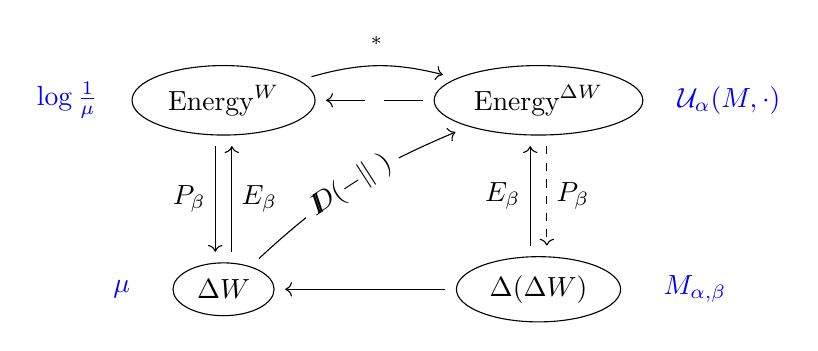
\begin{tikzpicture}
		%TODO left hand side of diagram, with worlds and mean parameters
		\node[ellipse,draw, outer sep=4pt] (DW) at (0,0) {$\Delta W$};
		\node[ellipse,draw, outer sep=4pt] (EW) at (0,2.4) {$\text{Energy}^W$};
		\node[ellipse,draw, outer sep=4pt] (DDW) at (4,0) {$\Delta (\Delta W)$};
		\node[ellipse,draw, outer sep=4pt] (EDW) at (4,2.4) {$\text{Energy}^{\Delta W}$};
		
		\node[right=0.5em of EDW, blue] {$\mathcal U_\alpha(\dg M, \cdot)$};
		\node[right=0.8em of DDW, blue] {$\bbr{\dg M}_{\alpha,\beta}$};
		\node[left=0.8em of DW, blue] {$\mu$};
		\node[left=0.5em of EW, blue] {$\log\frac{1}{\mu}$};
		
		\draw[->, transform canvas={xshift=3pt}] (DW) -- node[right]{$E_\beta$} (EW);
		\draw[->, transform canvas={xshift=-3pt}] (EW) -- node[left]{$P_\beta$} (DW);
		
		\draw[->, transform canvas={xshift=-3pt}] (DDW) -- node[left]{$E_\beta$} (EDW);
		\draw[->, dashed, transform canvas={xshift=3pt}] (EDW) -- node[right]{$P_\beta$} (DDW);
		
		\draw[->] (DW) to[bend left=10] node[sloped,fill=white]{$\thickD({-\Vert~})$} (EDW);
		
		\draw[->] (EW) to[bend left=15] node[above] {$\E^*$} (EDW);
		\draw[->] (EDW) to node[fill=white] {$\E$} (EW);

		\draw[->] (DDW) to node[below] {$\E$} (DW);
	\end{tikzpicture}}
	\caption{Energy / Distribution Transformations. 
		%The nodes are thermodynamic objects, the arrows are ways of constructing one from another
	}
	\label{fig:energies-and-dists}
\end{figure}
We now look at the weighted distribution semantics of PDGs from a thermodynamic perspective: this will provide better rationale for the parameter choices in \Cref{sec:scoring-semantics}, and draw some more explicit contrasts between PDGs and factor graphs.	Let $W$ be finite set of worlds, on which the distribution is supported, corresponding to a particle's possible ``micro-states''

Our technical starting point will be the Boltzmann distribution \eqref{eq:boltzmann}, which asserts that the probability $P$ of being in a state exponentially decreases as its energy $U$ increases; the rate of exponential decay is related to the ``inverse temperature'', $\beta$; here $Z_U(\beta)$ is a normalization constant. Fixing $\beta$, we can of course, invert the Boltzmann distribution \eqref{eq:invbolz}, obtaining an energy from a probability. A probability distribution over $W$ is called a configuration, or macro-state.
\begin{align}
 P_{\beta}(U) &:= w \mapsto  \frac{1}{Z_U(\beta)}\exp\Big(-\beta U(w)\Big) \label{eq:boltzmann} \\
	E_{\beta}(\mu) &:= w \mapsto \frac{1}{\beta} \ln \left(\frac{1}{\mu(w)}\right) \label{eq:invbolz}
%joe10*: I'm getting latex complaints again
\end{align}
Conversions between the two correspond to going up and down on the left of \Cref{fig:energies-and-dists}. 
Now $\mathcal U$, as defined in \eqref{eqn:full-score} is an un-normalized badness score, making it like an energy; $W^k_\gamma(\dg M, \mu)$, is a strangely-normalized Boltzmann distribution for this energy. The parameter $\beta$, which we described earlier as a certainty, plays the physical role of an inverse temperature: lower is more chaotic. 

$\mathcal U$ is not just an arbitrary construction either: it is analogous to a free energy. Why is the most favorable configuration not just a point mass as the minimum energy? Because in a world where an ambient temperature makes things more diffuse, doing things would require a lot more energy. Rather than just minimizing the average energy of a configuration $\nu$, you're better off minimizing the Gibbs free energy \eqref{eqn:gibbs-free-energy}. 
\begin{equation}
	G_E(\nu) = {\E}_\nu( E )  - T \H(\nu) \label{eqn:gibbs-free-energy}
\end{equation}
Analogously, why not put all of your weight on the one distribution you think is most likely? Because in a slightly chaotic world, doing so could actually incur a lot more inconsistency. Instead, we're better off minimizing $\cal U$. $\alpha$ is more transparently a temperature here, with higher values indicating higher preparedness for background chaos. 
% The higher order expectation we take in \eqref{eqn:higher-expectation} corresponds to the bottom edge of \Cref{fig:energies-and-dists}, and the diagonal, which is the natural way to construct free energies from a distribution, is a KL divergence. This can be seen directly, as well, in \Cref{ex:energy-from-distrib}.
%
See \ref{sec:thermo-background}, and
	\cite{bethe,friston2009free} for more comprehensive background
	on free energy 
%oli8
in graphical models.
%and \cite{} for weighted probability distributions.

A very weak version of this can already be seen in un-normalized factor graphs: by multiplying a factor $\phi$ by a constant $\alpha$, one obtains a free energy $G' = - \ln \alpha + G$, i.e., with a mere additive shift. However, this shift doesn't really distinguish belief states, which is part of why we're so eager to normalize the distribution.
There is also an opportunity to modify $\beta$, but in standard graphical model literature, people set $\beta = 1$ and forget about it.%
	\footnote{A similar complaint, is lodged in \cite{fixing-broken-elbo}, in which many information theoretic trade-offs are hidden by assuming $\beta = 1$}


\begin{example}%[continues=ex:worldsonly]
	\label{ex:energy-from-distrib}
	For the PDG $\dg M$ that encodes just a probability
			distribution $\mu$ over $W$,  $\Inc_{\dg M}(\nu) = \kldiv{\nu}{\mu}$. This quantity is also equal to $\mathcal G_{E(\mu)}$, the Gibbs free energy for the potential landscape associated to $\mu$ at temperature $\beta = 1$.
\end{example}


%oli8: modifications for correctness and to preserve references
%	A priori, \Cref{thm:free-energy-strictly-more-expressive} might be thought of as merely a novel function we came up with, but in fact this is not the case--- when the PDG is a Bayesian network, this is just the normal Gibbs free energy.
When the PDG corresponds to a Bayesian network, this is just variational Gibbs free energy of a distribution in the energy well constructed by the distribution specified by the BN.

\begin{prop}\label{prop:bn-free-energy}
	For any Bayesian Network $B$, 
	\[ \bbr{\PDGof{B}} = D(- || \Pr\nolimits_B) = \mathcal G_{E(\Pr_B)} \]
\end{prop}

By playing with thermodynamic parameters, the weighted distribution semantics coincide with the notions of free energy on standard graphical models; we therefore can view PDGs as implicitly providing a more expressive class of free energies, corresponding to weighted distributions, which in turn can be naturally adapted to be distributions themselves.

%	\begin{prop}
%		The Bethe free energy is equivalent to the Gibbs free energy of $M$ iff $M$ is strongly consistent.
%	\end{prop}


%	\begin{conj}\label{thm:free-energy-strictly-more-expressive}
%		The weighted distributions generated by PDGs are strictly more expressive than those generated by BNs, Factor Graphs, or directed factor graphs.
%	\end{conj}
%	\begin{proof}
%		The first two parts come from \Cref{thm:fg-free-energy,prop:bn-free-energy}. Since 
%	\end{proof}
%	\begin{coro}
%		Local minima of the Bethe free energy are fixed points of loopy belief propagation in PDGs		
%	\end{coro}


%joe7*: all the material after this will be cut, so you can focus
%(after we clean up the main part of the paper) on making the earlier
	%pat of the appendix comprehensible
%oli9: uncommenting so I can read this material, and reorganize slightly --- we'll need to shuffle around and cut a lot of appendix things in a bit but some of the good stuff is at the end.
% \commentout
{        
\section{Alternate Presentations}
%I think we finally covered this.
\commentout{\subsection{Random Variables}
If $\mathcal W = (W, \mathcal F, \mu)$ is a measure space, and $\mathcal X = \{ X_i: W \to \mathcal V(X_i) \}_{i \in I} $ is a collection of measurable random variables on $W$,\footnote{that is: $\mathcal V(X_i)$ is a measurable space, taking the form $(D, \mathcal D)$, and $X_i : W \to D$ is a set function such that for every $B \in \mathcal D$, the set $X_i^{-1}(B) \in \mathcal F$} and 
{\color{gray}$\Ed \subseteq I \times I$ is a collection of pairs of variables such that the agent is prepared to give  } 
\todo{what is a way of phrasing this that doesn't sound like it's shoehorned in? $\Ed$ really can represent anything an agent knows. Any subjective conditional probability distribution $\mu'$ such that the only measurable subsets are ``axis aligned'', in that they involve queries on only one variable, can be represented by $\Ed$, and for other queries we can simply change variables.}, we call $(\cal W, X)$ an \emph{ensemble}.
%and $(W, \mathcal F', p)$ is a subjective probability representing an agent's belief 


\begin{prop}
	There is a natural correspondence between strict PDGs as defined in \Cref{def:model}, and ensembles such that \todo{spell this out explicitly to avoid vague categorical intuition} \ldots $\mu$'s are defined on same set and produce same values.
\end{prop}
\begin{proof}
	\textit{/outline:}
	On the one hand, $(\prod_{N \in \cal N} \mathcal V(N).\text{set}, \bigotimes_{N \in \cal N} \mathcal V(N).\text{algebra}, \mat p)$ is a measure space, with $\{X_N = \pi_N : \left(\prod\mathcal V(N')\right) \to  \mathcal V(N) \}_{N \in \cal N}$ a set of random variables
	
	and  on the other, $(I, \Ed, \mathcal X', \mu|_{\cal L})$ is a strict PDG.
\end{proof}

This is the technical underpinning of our flippant, noncommittal treatment of possible worlds: any time we are thinking in terms of random variables or probability distributions on a fixed set $W$, we can instead reduce


The complexity of the representation is $O(XV + L V^2)$, compared to $O(XW)$}

\subsection{Hyper Graph Conversion}\label{sec:hyper-convert}
We have mentioned that the direct definition in terms of hyper-edges is possible; we give it below.

\begin{defn}[PDH]\label{def:hypermodel}
	A \emph{\modelnamehyper} is a tuple $\pdgvars[]$ where
	\begin{itemize}[nosep]
		\item $\N$~~is a finite collection of nodes
		\item $\Ed \subseteq 2^{\N} \times 2^{\N} \times \mathrm{Label}$~~is a set of directed edges, each of which has a source and target subset of $\N$.
		\item $\V$ associates each node $N \in \mathcal N$ with a set $\V(N)$ or $\V_N$, representing the values that node $N$ can take.
		\item $\bp$
		 % $\colon\!\big(\!({\bf A,B})\colon \! \Ed \big) \to \prod\limits_{A\in \bf A} \!\! \V(A) \to \underline\Delta\left[\prod\limits_{B \in \bf B}\!\!\V(B)\right]$
		%%% Above is the type of $\mat p$. I think it's important to have it there.
		associates conditional probability (sub)-distributions on the joint settings of $\bf B$ indexed by the joint settings of variables in $\bf A$ for every edge $({\bf A,B}) \in \Ed$. %
		% \note{The type of $\mat p$ is $\big(\!({\bf A,B})\colon \! \Ed \big) \to \V(A) \to \underline\Delta\V(B)$. It doesn't take up much space and answers lots of questions about the words above.}
	\end{itemize}
\end{defn}

	
The choice to formalize PDGs this way is a design consideration that makes some things cleaner, but we can just as well formalize multi-tailed edges directly, as follows:

\begin{defn}[PDH]\label{def:modelhyper}
A \textit{Probabilistic Dependency Hypergraph} (PDH) is tuple $(\N,
\mathbdcal{E}, \V, \bp)$ where $\N$ and $\V$ are as before, $\mathbdcal{E}
\subseteq 2^\N \times 2^\N \times \mathrm{Label}$ is a set of `hyperedges',
i.e., edges whose source and target are sets of nodes, and for each edge $L
= ({\bf A, B}, \ell) \in \mathbdcal{E}$, we have a table of distributions
$\bp$ on \emph{joint settings} of the variables in the set $\bf B$ for each
joint setting of the variables in $\bf A$.
\end{defn}

\Cref{thm:hyperequiv} shows PDGs and PDH s to be equivalent, though in different cases one may seem more natural than the other, as illustrated in the following theorem.

\begin{theorem}[restate=thmhyperequiv]\label{thm:hyperequiv}
	Every PDH $H$ is equivalent to a PDG $\dg M$ with additional variables. That is, for each semantics $\bbr{-}$ we define, $\bbr{H} = \bbr{\dg M}$.
\end{theorem}
\begin{proof}
	\todo{}
\end{proof}

This theorem justifies taking the PDG as primary, an ordinary collection of nodes and edges, which makes it cleaner to define and compose paths. 


\section{Formalism for other Graphical Models}
\begin{defn}
	A Baysian network (BN) is a tuple
	\[
	\mathcal B = \left(\mathcal N : \mathbf{FinSet}, ~~\mathrm{Par}: \mathcal N \to 2^{\mathcal N},~~ \mathcal S: \mathcal N \to \mathbf{FinSet},~~\Pr: \prod_{N : \mathcal N}  \left[ \mathcal S_N \times \left(\prod_{P : \mathrm{Par}(N)} \mathcal S_P\right)  \to [0,1] \right] \right)
	\]
	such that
	\begin{itemize}[nosep]
		\item the graph $\bigcup_{N, P \in \mathrm{Par}(N)}(N, P)$ is acyclic, i.e., there exists no cycle of nodes $N_0, N_1, \cdots, N_k = N_0$ in $\mathcal N^k$ such that $N_{i+1} \in \mathrm{Par}(N_i)$ for each $i \in \{0, 1, \cdots, k\}$.
		\item For all $N \in \mathcal N$, $\Pr(N)$ is a probability distribution on $\mathcal S_N$, i.e., 
		\[ \forall N\in \mathcal N.~\forall \vec{p} \in {\prod_{P : \mathrm{Par}(N)} \mathcal S_P}.~~ \sum_{n \in \mathcal S_{N}} \Pr_N(\vec{p}, n) = 1\]
	\end{itemize}
\end{defn}


\begin{defn} \label{def:bnconvert-formal}
	If $B = (\mathcal N, \mathrm{Par}, \mathcal S, \Pr)$ is a Bayesian Network, then let $\PDGof (B)$ denote the corresponding PDG given by the procedure in \Cref{sec:bn-convert}. Explicitly, 
	\[ \PDGof{{\mathcal B}} :=  (\mathcal N', \Ed, \mathcal V,
			\bp) \] 
	where % $\mathcal N'$ is the original nodes, plus
	\begin{align*}
	\mathcal N' &=  \left\{ \Big.\{N\} \mid N \in \mathcal N\right\} \cup \left\{ \mathrm{Par}(N) ~\middle|~ N \in \cal N \right\} \\%
	\Ed &= \left\{ \vphantom{\Big|}(\mathrm{Par}(N), \{N\}) \mid N \in \mathcal N \right\} \cup 
	\left\{\vphantom{\Big|} (P, \{X\}) \mid X \in P, P = \mathrm{Par}(N) \text{ for some }N \in \mathcal N \right\} \\
	\mathcal V_N &= \prod_{X \in N} \mathcal S_X \\
	%					{\color{gray}\Sigma_N = \bigotimes_{X \in N} 2^{\mathcal S_X}, \text{the product algebra of discrete $\sigma$-algebras}} \\
	\mathbf p &= \begin{cases}
	(\mathrm{Par}(N), \{N\}) &\mapsto \lambda(p, B).~ \displaystyle\sum_{b \in  B} \Pr(b \mid p) \\
	(P, X) &\mapsto, \lambda (p, B).~ \displaystyle \mathbbm 1_{\displaystyle\pi_X(p) \in B}
	\end{cases}
	\end{align*}
	%\cpm p(\frac{a}{z}|b)
\end{defn}
All we've done is explicitly add parent nodes and projection edges to our graph, and also subtly (by adding curly braces in the right places and taking unions rather than disjoint unions) eliminated the duplicate nodes arising from edges in the original BN which only have a single parent.

\section{Thermodynamics}\label{sec:thermo-background}
Let $W$ be a finite set of states.

\textbf{From Potentials to Distributions.}
Suppose $U: W \to \mathbb R$ is a potential function, assigning an energy to each state. Imagine there's a particle that could be in any number of states, that the only consideration in transitioning from one state $w$ to another $w'$ is the energy of each state,%
	\footnote{The thermodynamics, of course, ignore the kinetics of the system. Thought of an Ising model, the edges form a complete graph, and the edge weights are uniform. Thought of as a stochastic matrix, it is rank one, whose latent variable is just the energy of a state.}
and that low-energy states are more exponentially more likely,\footnote{this can also be replaced by weaker assumptions; see the thermodynamics literature for more motivation}
the unique stationary state is the Boltzmann distribution:
\begin{equation}
	 \mu(w) \propto \exp( - U(w) / kT ) \label{eq:boltzmann-appendix}
\end{equation}

where $k$ is the Boltzmann constant and $T$ is the thermodynamic temperature. Note that at unboundedly high temperatures, the differences between potentials don't matter (all states are equally likely), whereas at as the temperature approaches zero, the Boltzmann distribution puts zero mass on anything that's not a global minimum, and otherwise splits the mass equally. Therefore, if $U$ achieves a unique global minimum $w^*$, the corresponding $\mu(w) = \delta_{w,w^*}$ is a point mass on the minimum energy world $w^*$.

It is standard and notationally useful to re-parameterize with the inverse temperature $\beta := 1/kT$ -- and we will refer to the Boltzmann distribution associated to a given potential $U$ (and inverse temperature $\beta$) as 
\[ P_{\beta}(U) := w \mapsto  \frac{1}{Z_U(\beta)}\exp\Big(-\beta U(w)\Big) \]
Where $Z_U(\beta) = \sum_{w \in W} \exp(-\beta U(w))$ is a normalizing factor, sometimes called the ``partition function''.	

\textbf{From Distributions to Potentials}.	
On the other hand, under similar assumptions, if given a probability distribution $\mu$ over $W$, there is a natural potential energy that resulted in it, 
\[ E_{\beta}(\mu) := w \mapsto \frac{1}{\beta} \ln \left(\frac{1}{\mu(w)}\right)  \]
which might be recognizable as negative log liklihood or the ``surprise'' of an event happening. By construction, $P_\beta \circ E_\beta$ is the identity on probability distributions:
\begin{align*}
	 \Big(P_\beta \circ E_\beta(\mu)\Big) (w) &= \frac{1}{Z_{ E_\beta (\mu) }} \exp \left( - \ln \left(\frac{1}{\mu(w)}\right) \right) \\
	 &= \left(\frac{1}{\sum\limits_{w' \in W} \mu(w')}\right)\mu(w) \\
	 &= \mu(w)
\end{align*}
and $E_\beta \circ P_\beta$ is the identity on potential functions (up to a constant factor):
\begin{align*}
	\Big(E_{\beta}\circ P_\beta(U)\Big)(w) &= \frac{1}{\beta} \ln \left(\frac{1}{\frac{1}{Z_U(\beta)}\exp(-\beta U(w))}\right) \\
	&=  \frac{1}{\beta} \Big[\ln Z_U(\beta) - (-\beta U(w)) \Big]\\
	&= U(w) + \frac{1}{\beta} \ln Z_U (\beta)
\end{align*}
The constant factor $-\frac{1}{\beta} \ln Z_U(\beta)$ coincides with the Heimholtz free energy of the system. Note that at constant temperature, this quantity is a durable feature of either a distribution or its associated energy landscape. 
%	
%	\begin{align*}
%		 0 = -\frac{1}{\beta} \ln Z_U(\beta) &= - \frac{1}{\beta} \ln \sum_{w \in W} \exp(-\beta U(w)) \\
%		 \iff 1 = \sum_{w \in W} \exp(-\beta U(w))
%%		 	&= -\frac{1}{\beta} \mathop{\mathrm{LSE}}_{w \in W}(-\beta U(\beta))
%	\end{align*}

\textbf{Free Energy and Favorability.} Given a potential $U$, corresponding to a distribution $\mu$ as above, we now turn the question of how thermodynamically favorable a new distribution $\nu$ would be.%
	\footnote{From a statistical mechanics perspective, $W$ are the micro-states of the system, and a distribution over them is a configuration, or a macro-state.}
For which we use the Gibbs free energy, $G_U(\nu) := {\E}_\nu( U ) - \frac{1}{\beta} H(\nu)$, which we think of a system as minimizing. The intuition here is that our new distribution $\nu$ is favorable if it has low average energy. However, at higher temperatures it also costs energy to compress the distribution: while a point mass at the minimum value of $U$ may be the lowest energy distribution, tightly controlling it to that degree also costs energy, when there's some ambient temperature causing randomness. From an epistemic perspective, even if a belief distribution $p$  is the one that best fits constraints, one might want to temper this by other possible configurations, and more so when there's higher ambient macroscopic uncertainty (temperature). Note also that the Gibbs Free Energy is a weighted probability distribution: it assigns a `favorability' score to distributions.

If $U$ was generated by a probability distribution $\mu$, we then have

\begin{align*}
	G_\mu(\nu) &= {\E}_\nu( E_\beta(\mu) )  - T S(\nu) \\
	&= \sum_{w \in W}\nu(w) \frac{1}{\beta} \ln \left(\frac{1}{\mu(w)}\right) - T \left[k \sum_{w \in W} \nu(w) \ln \left(\frac{1}{\nu(w)}\right)\right]\\
	&=  \frac{1}{\beta}\left[\sum_{w \in W}\nu(w) \ln \left(\frac{1}{\mu(w)}\right) - \sum_{w \in W} \nu(w) \ln \left(\frac{1}{\nu(w)}\right)\right]\\
	&=  \frac{1}{\beta}\left[\sum_{w \in W}\nu(w) \left(\ln \frac{1}{\mu(w)} - \ln \frac{1}{\nu(w)}\right)\right]\\
	&= \frac{1}{\beta} D \left(\nu || \mu \right)
\end{align*}

Where $D(\nu || \mu)$ is the relative entropy from $\nu$ to $\mu$. 

Note that by Gibbs inequality, the $D(\nu || \mu) \geq 0$, and equal to zero precisely when $\nu = \mu$, and so the free energy of a configuration $\nu$ in a potential that was designed for $\mu$ is minimized by $\mu$ itself.	



\textbf{Free Energy as a Design Tool.}

This connection between thermodynamics and probability theory is already well utilized:
\begin{enumerate}
	\item A Markov Random Field is specified with potentials $U_e$ for each edge; a factor graph is specified with potentials for a subset of cliques.
	\item The belief propagation algorithm computes local minima of the Bethe free energy, an approximation to the true Gibbs free energy.
\end{enumerate}


The dominant representation tool for mental states is the probability distribution, rather sets or weighted sets of them. % This is partly because they are easier to compute with, and because when faced with decisions at gun point, they are the most
One issue with this is that there are distinct mental states that collapse to the same probability distribution (e.g., the coin flip: being uncertain about a process vs its outcome). The second one is that one might not have the right space for the distribution

The insight here is that these are related: one can simply internalize the structure of the uncertainty. This some precedent for this: Pearl's rule, for instance, prescribes a new random variable to describe the uncertainty.	
%%%

%	Consider a factor graph on a set of variables $\{ X_i \}$, with only a single factor $\phi$ which connects to every variable. The free energy is $G_\phi(U)$
%	
%	\[ \frac{1}{\sum_{\vec x} \phi(\vec x)} \phi(u) \]
%	
%%	The normalization constant $Z = \sum_{\vec x} \phi(\vec x)$
%	
%	Any factor graph defines a free energy by \todo{finish}
%	
%	The Bethe approximation to the free energy is an estimate based only on the marginals on single pairs of nodes.
%		
%	With a PDG, the free energy becomes
%	\[ \sum \]
%	\todo{Write out $\Inc$, proofs of theorems}


\section{Overview And Conversions Between Graphical Models}
\label{sec:many-relations-graphical-models}

\usetikzlibrary{decorations.markings}	
\begin{figure*}[t]
	\centering
	\tikzset{attn/.style={draw, fill=magenta, fill opacity=0.3, font=\Large\slshape\color{blue}, inner sep=4pt}}
	\scalebox{0.75}{
		\begin{tikzpicture}
		\begin{scope}[every node/.style={ellipse, fill, fill opacity=0.05,text opacity=1,
				outer sep=3pt,font=\slshape\color{blue}}, xscale=2.5,yscale=1.2]
			\node (KB) at (-3, 0.5) {KB};
			\node (CG) at (-3, 1.5) {CG};
			
			\node (CRF) at (-1.2, 0.4) {CRF}; % CFG
			%				\node (CRF) at (-2, 0) {CRF};
			
			\node (MRF) at (-2, 1) {MRF};
			\node[draw, attn] (FG) at (-1,1.35) {FG};
			\node (SDFG) at (0,1.5) {FG$^\rightharpoonup$};
			\node[attn] (DFG) at (1,1.35) {FG$^\rightarrow$};
			\node[attn] (BN) at (2,1) {BN};
			
			\node (CBN) at (2,0) {CBN};
			\node (DN) at (1.3, 0.6) {DN}; 
			
			\node (sPDGH) at (0,0.5) {sPDG$_{\text{hyper}}\!\!$};
			\node (PDGH) at (-0.8,-.5) {PDG$_{\text{hyper}}\!\!\!$};
			\node (PDG) at (0,-.85) {PDG};
			\node[attn, fill=black, fill opacity=0.9, text=white] (sPDG) at (0.8,-.5) {sPDG};
			
			\node (prog) at (3, -0.2) {PProgSet};
			
			\node (CPS) at (1, -1.4) {CPS};	
			\node (PlateBN) at (-2.5, -1.2) {PlateBN};
			\node (LPS) at (-1,-1.4) {$\underline {\mathcal P}$};
		\end{scope}
		
		% lossless		
		\begin{scope}[every edge/.append style={->}]%right hook->
			\draw (BN) edge (DFG) (DFG) edge (SDFG);
			\draw (MRF) edge (FG) (FG) edge (SDFG);
			%				\draw[->] (DFG) -- (FG);
			\draw (CBN) edge[bend left = 5, shorten >=7pt] (sPDGH);
			\draw (CG) edge[bend left=10] (FG);
			\draw (KB) edge (CG);
			
			\draw (sPDGH) edge (PDGH) (sPDG) edge (PDG);
			
			\draw (BN) edge (DN) (DN) edge (sPDGH);
			\draw (DFG) edge (sPDGH);
			
			\draw (MRF) edge (CRF);% (CRF) edge (CFG);
			\draw (BN) edge (CBN);
			\draw (FG) edge (CRF); %crf
			
			\draw (CG) edge[out=-55, in=195, looseness=1.5, shorten >=7pt] (sPDGH);
			\draw (prog) edge[bend left=5] (sPDG);
			\draw (CPS) edge[out=180,in=-30] (PDG);
			\draw (PlateBN) edge[bend right=5] (PDGH);
			\draw (LPS) edge[out=0, in=-150] (PDG);
		\end{scope}
		
		% PDG Equivalences
		%			\draw[->, transform canvas={yshift=2pt}] (PDGH) -- (PDG);
		%			\draw[->, transform canvas={yshift=-2pt}] (PDG) -- (PDGH);
		%			
		%			\draw[->, transform canvas={yshift=2pt}] (sPDGH) -- (sPDG);
		%			\draw[->, transform canvas={yshift=-2pt}] (sPDG) -- (sPDGH);
		
		\draw[double equal sign distance, shorten <=0pt, shorten >=0pt] (PDGH) -- (PDG);
		\draw[double equal sign distance] (sPDGH) -- (sPDG);
		
		
		% Projections. Lose information but preserve something.
		\begin{scope}[every edge/.append style={densely dashed, orange, ->}]
			\draw (sPDGH) edge[bend left=10, out=10] (FG) (sPDGH) edge[bend right=10, out=-5] (FG);
			\draw (SDFG) edge[bend right=20] (FG);
		\end{scope}
		% Inefficient conversions.
		\begin{scope}[every edge/.append style={ultra thick, dotted, line cap=round, shorten >=2pt,
				decoration={markings,mark=at position 1 with {\arrow[xshift=0pt,scale=.8]{>}}},
				postaction={decorate}}]
			\draw (CRF) edge (sPDGH);
			\draw (SDFG) edge (sPDGH);
		\end{scope}
		
		%			\draw[->, transform canvas={xshift=-3pt}] (DDW) -- node[left]{$E_\beta$} (EDW);
		%			\draw[->, dashed, transform canvas={xshift=3pt}] (EDW) -- node[right]{$P_\beta$} (DDW);
		%			
		%			\draw[->] (DW) to[bend left=10] node[sloped,fill=white]{$D({-\Vert})$} (EDW);
		%			
%joe10: I get latexerors from the subfiglabelcolor
%oli12: I did a poor find-and-replace to replace blue with this earlier and it broke when you commented out my figure. 
			\end{tikzpicture}
	}
	\caption{Transformations Between Graphical and Epistemic Models. Solid arrows indicate a model being a special case of another. Orange dashed transformations lose information, and the thick arrows are inefficient translations. For a full description, check \Cref{sec:many-relations-graphical-models}. }
	\label{fig:model-transformations}
\end{figure*}
\todo{There is a ton to do here.}

\subsection{The Details: Factor Graphs and PDGs} \label{sec:factor-graphs-long}
% What I want to see is a serious discussion of the advantages and disadvantages of factor graphs vs. PDGs, illustrated by examples. This is critical.


We now compare PDGs with factor graphs, a general class of \emph{undirected} graphical models, often described as a generalization of BNs and Markov Networks.
%todo: hint at MN relation in beginning. 
%PDGs can simulate them (\cref{def:fg-convert}), but not without large cpds and sneaky use of inconsistency. 


%% informal, unclear.
\begin{quickdefn}
A \emph{factor graph} is a collection of random variables $\mathcal X = \{X_i\}$ and a collection of \emph{factors} $\{\phi_\alpha\colon X_\alpha \to \mathbb R_{\geq0}\}_{\alpha \in \mathcal I }$ over subsets $\alpha$ of $\mathcal X$.
\end{quickdefn}
\begin{defn}
%oli6: I have removed my "intuitive" cavalier version of the definition 
% that you disliked (which has often been given in technical
% overviews I've read, but bugs me by leaving things undefined so I
% expanded it, but left a short version for people who aren't interested
% in following the technical details closely).
	% A \emph{factor graph} on variables $\{X_j\}$ is a set of \emph{factors} $\{\phi_\alpha\colon X_\alpha \to \mathbb R_{\geq0}\}_{\alpha \in \mathcal I }$ over subsets $\alpha$ of the variables.
	% 
	% More precisely, a
	A factor graph $ (\{\phi_\alpha\}_{\alpha \in \cal I})$ on an indexed set of random variables $\mathbf X = \{ X_j \}_{j \in J}$, 
%oli6:
% I know the \iota bothers you, but I did think about this for a long
% time, and think this is the cleanest presentation that can be
% perfectly formalized without relying on any notions of equality
% between natural objects, or lack of formality when constructing
			% them.
%joe6: Most people don't use it, right?  There's a good reason...
%Why would it hurt to do things the way Koller and Friedman do?                
%Since I think that ultimately factor graphs will play only a small
%role in the paper, we should use the simplest possible presentation
%of them.  I don't mind being slightly informal.
	is a pair $((\mathcal I,\iota), \boldsymbol\phi)$, where $\cal I$ is a set,
	each element $\alpha\notation{\in \mathcal I}$ of which determines a selection $\iota(\alpha) \subseteq J$ of the variable indices, and
	$\boldsymbol\phi$ is an indexed collection of \emph{factors} $\{\phi_\alpha\}_{\alpha \in \mathcal I }$, 
	where each factor $\phi_\alpha \colon \mathcal X_\alpha \to \mathbb R_{\geq 0}$ assigns a non-negative score to joint settings $\vec x_\alpha \notation{\in \mathcal X_\alpha}$ of every variable in $\iota(\alpha)$, all values of which we denote by $\mathcal X_\alpha\notation{ := \prod_{j \in \iota(\alpha)} \mathcal V(X_j)}$. 
\end{defn}
\begin{fulldefn}
A \emph{factor graph} $(\mathcal I, \phi)$ on an indexed set of random variables $X : \Sigma_{}$, where each $X_i$ can take values $\V(X_i) =: \mathcal X_i$, consists of  
% technically, a dependent sum \mathbb X : \Sigma_{j : J} X_j
%		a set $\cal I$, where each $\alpha \in \cal I$ is a
% technically a multi-subset of 2^J...
a set of \emph{factors} $\{\phi_\alpha\}_{\alpha \in \mathcal I }$, where each $\alpha$ determines a selection $\iota(\alpha) \subseteq 2^J$ of the variable indices, and the associated factor $\phi_\alpha \colon \mathcal X_\alpha \to \mathbb R^{\geq 0}$ assigns a non-negative score to a setting
$\vec x_\alpha \in \mathcal X_\alpha := \prod_{j \in \iota(\alpha)} \mathcal X_j$ of the variables corresponding to $\iota(\alpha)$.

\end{fulldefn}

% $(J, \mathcal I)$
While the qualitative structure $(\mathbf X, \mathbf{Pa})$ of a BN on variables $\mathbf X$ is a directed acyclic graph, the qualitative structure $(\mathbf X, \mathcal I)$ of a factor graph on $\mathbf X$ is
%		technically an undirected \emph{multi-hyper-graph}
%	 		\footnote{That is, a set of ``nodes'' $\N$ and
%a collection (possibly containing multiple copies) of ``hyper edges''
	%$\Ed$, each of which corresponds to a subset of $\N$}
%joe4*: what is a multi-hypergraph?   Is this by analogy to a
%multigraph, there can be multiple hyperedges joining the same set of
%nodes? Either explain the ``multi'' or remove it.
%oli5: This is correct. I think this might actually be standard for a hyper-graph though, so I don't feel bad about removing it; just wanted to be precise.
a hypergraph $(\mathbf X, (\cal I, \iota))$ where
	$\alpha \in \cal I$ is an undirected hyperedge, drawn as a
	square, connecting the vertices in the set $\iota(\alpha)$.  
%	a bipartite graph $((\mathbf X, \cal I), \iota)$ with extra vertices (drawn as squares) corresponding to the factors. 

%	\note{Though easier to define in terms of MRFs, and this obscures the relationship to BNs and MRFs; this  paper in particular is an attempt to claim that adding and removing nodes is not something to sweep under the rug.}



%	The important thing about 
A factor graph $\Phi = (\{\phi_\alpha\}_{\alpha \in \cal I})$ on $\mathbf X$ defines a probability distribution over $\V(\mathbf X)$ by 
\begin{align*}
%joe6: I have never seen the :\alpha notation before.  Unless it's
%standard, just use \alpha.  It also doesn't make sense to have both
%\alpha and =.  Let's just simplyify it
%		\Pr\nolimits_\Phi(\vec x) &:\propto \prod_{\alpha \in
	  %                  \cal I} \phi_\alpha(\vec x_{\alpha})
%          		~~= \frac{1}{Z_\Phi} \prod_{\alpha \in \cal I}
			\Pr\nolimits_\Phi(\vec x) 
	= \frac{1}{Z_\Phi} \prod_{\alpha \in \cal I}
							\phi_\alpha(\vec x_{\alpha}), 
\end{align*}
where $\vec{x}$ is a joint setting on all of the variables, $\vec{x}_\alpha$ is the restriction of $\vec{x}$ to only the variables selected by $\alpha$, and $Z_\Phi$ is the constant required to normalize the distribution. 
%joe4
%	There are several ways of parameterizing factor graphs; we
%        start with the most explicit one. 
	
%joe4*: I'm missing the big picture here.  What's the goal?  You've
%defined factor graphs.  What more do you need.  (I don't mean to
%imply that there isn't more that you might want/need, just that I
%don't know what it is.)
%joe4: I don't understand what it means that ``the particular setting of
%which matter''.  And I'm not sure what global/local would mean here.
%This is a fair complaint, this is not very well-explained.
%even though the
%        particular settings of which do matter, the interactions are
%        global and it's hard to see how they will play out. Still,
%joe4: I don't see how factor graphs are excellent desriptions of
%independencies  This has to be explained better.
%        they are excellent descriptions of independencies. 
%	 David's score is independent of everything else in the picture, and though the other three are a clique, we can see different interactions

%joe4
%Any BN $\mathcal B = (\N, \Pa, \V, p)$ can be seen naturally
A BN $\mathcal B = (\N, \Pa, \V, p)$ can be viewed
as a factor graph, which we denote $\Phi(\mathcal B)$.
%joe4: while the next line is true, do we need it?  Why not just
%explain directly how a BN can be viewed as a factor graph.
%oli5: I'm not sure what you're asking for. Writing down the global
% semantics is a clear demonstration that it's a product of factors. 
% I'm reinstating what I had, plus some minor modifications to clarify
%joe6: are there also local semantics?
%By the global semantics of BNs, we have that
By the semantics of BNs, we have that
\begin{align*}
% joe4: to get the \B to be positions right relative to the \Pr.  But I think that we should cut this anyway
  % \Pr\nolimits_{\cal B}(\vec x) = \prod_{N \in \N} p_N( \vec x_N
  {\Pr}_{\cal B}(\vec x) = \prod_{N \in \N} p_N( \vec x_N
	 \mid \mathbf{Par}_N(\vec x)). 
\end{align*} 
%joe4: please fill in the blank below, and avoid using \iota
%oli5: \iota is part of my definition, but it's a pretty obvious
% identification so I can just not mention it if that's better...
%	 Factors can be read off directly: set $\cal I = \N$, connect every
% 	variable $X$, and all of its parents $\Pa_X$, to the factor
% 	corresponding to $X$, by $\iota(X) := \{X\} \cup \Pa_X$. Finally,
%	define the function $\phi_X(x, \vec{y}) := p_X( X \!\!=\!\! x \mid
%	\Pa_X \!\!=\!\! \vec y)$ to simply be the cpd at $X$.
%
%joe6: Is this what you meant?
%Factors can be read off directly: set $\cal I = \N$, connect every
%variable $X$, and all of its parents $\Pa_X$, to the factor
%corresponding to $X$%
In the factor graph correponding to ${\cal B}$, 
we set $\cal I = \N$, and have a factor for every variable $X$, which
consists of $X$ and all its parents in ${\cal B}$.
%oli5: it's still intelligable without this line, just not complete. 
%, by $\iota(X) := \{X\} \cup \Pa_X$
%joe6
%Finally,
%define the function $\phi_X(x, \vec{y}) := p_X( X \!\!=\!\! x \mid
We define $\phi_X$ by taking
$\phi_X(x, \vec{y}) := p_X( X \!\!=\!\! x \mid
%joe6
%\Pa_X \!\!=\!\! \vec y)$ to simply be the cpd at $X$.
\Pa_X \!\!=\!\! \vec y)$; that is, $\phi_X$ is determined by the cpd of $X$.
%joe6: this seems redundant
%The corresponding factor graph has the same set of variables, and a
%hyperege corresponding to each node, which connects a node $X$ to its
%parents.
The factor $\phi_X$ correspond to the node $X$ is given by the cpd of
$X$; that is, $\phi_X(x,
\vec{y}) := p_X( X \!\!=\!\! x \mid 
\Pa_X \!\!=\!\! \vec y)$.
%joe4:
%Examples of this can be seen in the solid components of
%\Cref{subfig:fg-gf,subfig:fg-smoking}, which correspond to the initial
%
\Cref{subfig:fg-gf,subfig:fg-ablate,subfig:fg-smoking} give the factor graphs corresponding  to
the BNs in \Cref{ex:guns-and-floomps,ex:grok-ablate,ex:smoking}, respectively.  
%\Cref{subfig:fg-gf,subfig:fg-smoking}, which correspond to the initial
%to BNs in \Cref{ex:guns-and-floomps,ex:smoking}, respectively. 


\begin{figure}[htb]
	\centering
	\begin{subfigure}[b]{0.22\linewidth}
		\scalebox{0.8}{
			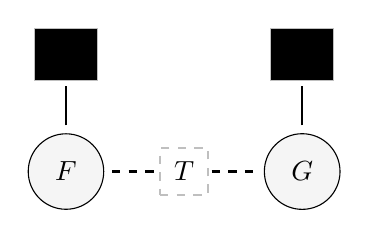
\begin{tikzpicture}[center base]
				\node[fgnode] (F) at (-1.5,0) {$F$};
				\node[fgnode] (G) at (1.5,0) {$G$};
				\node[factor, above=0.5 of F] (f) {$\phi_F$};
				\node[factor, above=0.5 of G] (g) {$\phi_G$};
				
				\draw[thick] (F) -- (f) (G) -- (g);
				\draw[thick, dashed] (F) -- node[factor, fill=white]{$T$} (G);
		\end{tikzpicture} }
		\caption{}\label{subfig:fg-gf}
	\end{subfigure}%
	\hspace{1.5em}\vline\hspace{1.5em}%
	\begin{subfigure}[b]{0.3\linewidth}
		\scalebox{0.8}{
			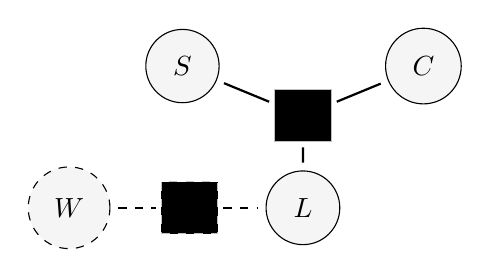
\begin{tikzpicture}[center base, scale=0.9]
				\node[fgnode] (S) at (-0.4, 2) {$S$};
				\node[fgnode] (C) at (3, 2) {$C$};
				\node[fgnode] (L) at (1.3,0) {$L$};
				\node[fgnode, dashed] (W) at (-2,0) {$W$};
				
				\node[factor] (f1) at (1.3, 1.3){$\phi_1$};
				\node[factor, dashed] (f2) at (-0.3, 0){$\phi_2$};
				
				\draw[thick] (S) -- (f1) -- (C) (f1) -- (L);
				\draw[thick, dashed] (W) -- (f2) -- (L);
		\end{tikzpicture} }
		\caption{}\label{subfig:fg-ablate}
		
	\end{subfigure}%
	\hspace{1.5em}\vline\hspace{1.5em}%
	\begin{subfigure}[b]{0.3\linewidth}%
		%			\vspace{-1em}
		\scalebox{0.72}{
			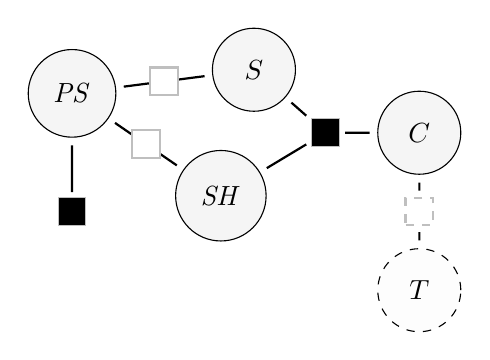
\begin{tikzpicture}[center base, xscale=1.4,
				fgnode/.append style={minimum width=3em}]
				\node[factor] (prior) at (1.65,-1) {};
				\node[factor] (center) at (3.95, 0){};
				
				\node[fgnode] (PS) at (1.65,0.5) {$\mathit{PS}$};
				\node[fgnode] (S) at (3.3, 0.8) {$S$};
				\node[fgnode] (SH) at (3.0, -0.8) {$\mathit{SH}$};
				\node[fgnode] (C) at (4.8,0) {$C$};
				
				\draw[thick] (prior) -- (PS);
				\draw[thick] (PS) --node[factor, fill=white](pss){} (S);
				\draw[thick] (PS) --node[factor, fill=white](pssh){} (SH);
				\draw[thick] (S) -- (center) (center) -- (SH) (C) -- (center);
				
%					\node[dpadded, fill=blue] (1) at (2.5,-2) {1};
%					
%					\draw[blue!50, arr] (1) -- (prior);
%					\draw[blue!50, arr] (1) -- (center);
%					\draw[blue!50, arr] (1) -- (pss);
%					\draw[blue!50, arr] (1) -- (pssh);
				
				
				\node[fgnode, fill opacity=0.02,dashed] (T) at (4.8, -2) {$T$};
				\draw[thick,dashed] (T) -- node[factor, fill=white]{}  (C);	
		\end{tikzpicture}}
		\caption{}\label{subfig:fg-smoking}
	\end{subfigure}%
	\caption{Candidate factor graphs for \Cref{ex:guns-and-floomps,ex:grok-ablate,ex:smoking}.
%oli10: no light blue here anymore
%The light blue arrows illustrate \Cref{def:fg2PDG}.
	}
	\label{fig:fg-intro-examples}
\end{figure}

%joe6: I couldn't parse your English, so I wrote what I thought you meant:
%	This suggests an obvious way to view an arbitrary collection
%        of cpds in the form of a PDG $\dg M$ as a factor graph
%        $\Phi(\dg M)$: just like for a BN, ignore the directions of the
	%        edges and use the cpds as factors.
We can apply this way of viewing BNs as factor graphs to arbitrary
PDGs: we take the factors to be defined by the cpds.
\begin{defn}[PDG to factor graph]
	If $\dg M = \pdgvars[]$ is a PDG, define 
%joe6*: Sorry, I don't undestand this notation.  Is ((\Ed,\in), \mat
%p)$ supposed to be a factor graph? So you're somehow identify \in
%with \iota?  This shows that the use of \iota is making life worse
%...  I think that you have to spell this out better.
	$ \Phi(\dg M) := ((\Ed,\in), \mat p)$
	to be the associated factor graph on the random
			variables $(\N, \V)$. 
\end{defn}
%joe6*: I didn't follow this remark.  I think that you want here is a
%simple theorem about how the PDG and the associated factor graph
%define the same distribution.  Is that even true?  If so according
%to what semantics.  If not, then in what sense are the two related.
%I an unhappy about this story.
\begin{remark}
	It is easy to verify that this construction yields the 
			same product of factors, whether one thinks of a PDG
			as a hypergraph directly, or translates it to a graph
			first, as formalized in \Cref{sec:formal+syntax}. 
\end{remark}

%joe6*: Why do I care about inverting this process.  Again, I think
%that this is not a good story.  I'm not reading the rest of this
%carefully, since  I don't think we'll want to keep it.      
In order to faithfully invert this process, converting a
	factor graph to a PDG, we would need to arbitrarily chose a
	direction for each edge and normalize; the different
	directions may result in wildly different distributions, none of
	which are necessarily related to the distribution determined
	by the original factor
	graph. We can do much better by giving up on creating
%joe4*: I don't understand what the figure is showing me.  Ae we
%getting different graphs?  It looks like we're getting just one PDG.
%Moreover, Definition 4.4 also seems to get one PDG.
%oli5: It is just one PDG. They're all one PDG. This paragraph was
%intended to show that choosing a direction is NOT a tenable way to
%construct a PDG from a factor graph, thereby explaining why we can't
%totally invert the process we used to get there, and explaining why
%they're all connected to \sf 1. 
	the \emph{same} graph, as illustrated in \Cref{fig:fg2PDG} and
	defined below.  

\begin{figure}[htb]
	\centering
%		\begin{subfigure}{0.5\linewidth}\centering
%			\scalebox{0.72}{
%				\begin{tikzpicture}[center base, xscale=1.4,
%					fgnode/.append style={minimum width=3em}]
%					\node[factor] (prior) at (1.65,-1) {};
%					\node[factor] (center) at (3.95, 0){};
%					
%					\node[fgnode] (PS) at (1.65,0.5) {$\mathit{PS}$};
%					\node[fgnode] (S) at (3.3, 0.8) {$S$};
%					\node[fgnode] (SH) at (3.0, -0.8) {$\mathit{SH}$};
%					\node[fgnode] (C) at (4.8,0) {$C$};
%					
%					\draw[thick] (prior) -- (PS);
%					\draw[thick] (PS) --node[factor, fill=white](pss){} (S);
%					\draw[thick] (PS) --node[factor, fill=white](pssh){} (SH);
%					\draw[thick] (S) -- (center) (center) -- (SH) (C) -- (center);
%					
%					%					\node[dpadded, fill=blue] (1) at (2.5,-2) {1};
%					%					
%					%					\draw[blue!50, arr] (1) -- (prior);
%					%					\draw[blue!50, arr] (1) -- (center);
%					%					\draw[blue!50, arr] (1) -- (pss);
%					%					\draw[blue!50, arr] (1) -- (pssh);
%					
%					
%					\node[fgnode, fill opacity=0.02,dashed] (T) at (4.8, -2) {$T$};
%					\draw[thick,dashed] (T) -- node[factor, fill=white]{}  (C);	
%			\end{tikzpicture}}
%		\end{subfigure}
%		\begin{subfigure}{0.5\linewidth}\centering
		\scalebox{1}{
			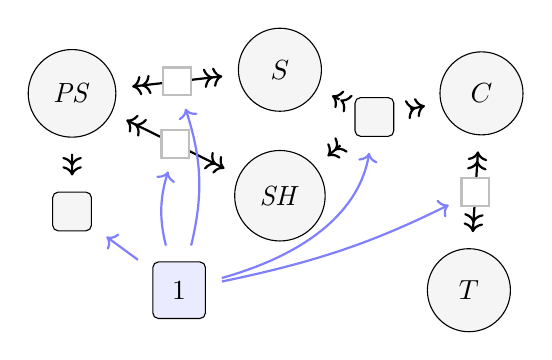
\begin{tikzpicture}[center base, xscale=1.6,
				fgnode/.append style={minimum width=3em}]
				\node[dpadded] (prior) at (1.65,-1) {};
				\node[dpadded] (center) at (4.05, 0.2){};
				
				\node[fgnode] (PS) at (1.65,0.5) {$\mathit{PS}$};
				\node[fgnode] (S) at (3.3, 0.8) {$S$};
				\node[fgnode] (SH) at (3.3, -0.8) {$\mathit{SH}$};
				\node[fgnode] (C) at (4.9,0.5) {$C$};
				
				\draw[arr, <<-] (prior) -- (PS);
				\draw[arr, <<->>] (PS) --node[factor, fill=white](pss){} (S);
				\draw[arr, <<->>] (PS) --node[factor, fill=white](pssh){} (SH);
				\draw[arr, <<-] (S) -- (center); 
				\draw[arr, <<-] (SH)-- (center); 
				\draw[arr, <<-] (C) -- (center);
				
				\node[dpadded, fill=blue] (1) at (2.5,-2) {1};
				
				\draw[blue!50, arr] (1) -- (prior);
				\draw[blue!50, arr] (1) to[bend right=30] (center);
				\draw[blue!50, arr] (1) to[bend right = 10] (pss);
				\draw[blue!50, arr] (1) to[bend left = 10] (pssh);

				
				\node[fgnode] (T) at (4.8, -2) {$T$};
				\draw[arr, <<->>] (T) -- node[factor, fill=white](tc){}  (C);	

				\draw[blue!50, arr] (1) to[bend right = 10] (tc);
		\end{tikzpicture}}
%		\end{subfigure}
	
	\caption{A graphical illustration of the conversion from a factor graph (the one shown in \Cref{subfig:fg-smoking}) to a PDG, as defined in \Cref{def:fg2PDG}. The blue edges carry the cpds corresponding to the original factors, and the structure is turned into the double headed deterministic black arrows.}
	\label{fig:fg2PDG}
\end{figure}

\begin{defn}[factor graph to PDG] % \label{def:fg2PDG}
	If $(\{\phi_\alpha\}_{\alpha \in \cal I})$ is a factor graph, then let $\PDGof{\Phi}$ be the PDG generated by inserting joint variable node $X_\alpha = \prod_{j \in \iota(\alpha)} X_j$ for every factor node $\alpha \in \mathcal I$ (as done in \Cref{def:bn2PDG}), and an edge $\sf 1 \to X_\alpha$ whose associated cpd $\bp[\alpha]$ is the joint distribution on the variables corresponding to $\alpha$ obtained by normalizing $\phi_\alpha$ across all of their possible values.%
\end{defn}


\begin{prop}\label{prop:fg-pdg-lossless}
	$\Phi \circ \PDGof = \mathrm{Id}_{\text{FG}}$. That is, if $F$ is a factor graph, then $\Phi(\PDGof{F}) = F$.
\end{prop}
\begin{proof}
%joe4: what's a local normalization?      
%oli5: we are required to normalize each cpd 1->X because they are
%distributions. It's local because it's done for each cpd, and these
%normalizations are unlikely to ultimately be compatible with the
%joint distributions on these variables.    
	Because each local normalization results in a local joint
			distribution $\bp[\alpha] = \frac{1}{Z\alpha}
%joe4*: I'm confused.  What differs from what?  is this what you meant
%                \phi_\alpha$, which only differs by a multiplicative
%               constant, their product will only differ by a
%oli5: You're right, this was super unclear. I rewrote to clarify.
			\phi_\alpha$ on the variables associated with $\alpha$, and these distributions differ from the original factors $\phi_\alpha$ by only a multiplicative 
		   constant, the product of these locally normalized factors differs from the product of the factors by only a constant, and so 
	\[ \Pr_F(\vec x) \propto \prod_\alpha \phi_\alpha(\vec x) \propto \prod_\alpha \left(\frac{\phi_\alpha(\vec x)}{Z_\alpha}\right) \propto \Pr_{\Phi(\PDGof{F})}(\vec x) \]
	and since the two distributions are normalized, they must be equal.
\end{proof}

%oli6: expanding a lot here to tell the story better.
% 	This suggests that the PDG has all of the information we need
% 	to interpret the factor graph.
% However, the distribution $\UD{\PDGof{F}}$ that PDG semantics prescribe may
% look nothing like $\Pr_F$ (cf.~\Cref{ex:fg-exam}). 

It may be surprising that a factor graph can be \emph{losslessly} converted to a PDG in a reasonable way, given that PDGs are directed models.
This fact suggests that $\PDGof{F}$ contains all of the same information as $F$. Knowing also that BNs are a kind of factor graph, it is natural to wonder if the unique distribution $\bbr{\PDGof{F}}^*$ given by our semantics, is the same as $\Pr_F$.		


% For the time being, it is important just to note that the
% distribution $\UD{\PDGof{F}}$ that PDG semantics prescribe may
% look nothing like $\Pr_F$ (cf.~\Cref{ex:fg-exam}). 
	
However, it is closely related---it turns out that by merely providing different weights for the terms in \Cref{eqn:full-score}, we can recover the probability distribution. Better still, this construction will litterally match the factor graph of equivalent of the scoring function $\mathcal U_\gamma(\dg M)$ (called the free energy, for reasons detailed in \Cref{sec:thermo}).
%oli6: When should I get people thinking about U being a free energy? 
% Ideally I want to point to the connection between them here, and I want to get people thinking
% thinking of "free energy" this way as soon as possible without losing them. 
%oli6: end of expansion, remove paragraph break.
%
%oli6: completely rewrote paragraph.
% In \Cref{sec:fg-expfam}, we break down the full semantics $\bbr{-}$
% of a PDG to show exactly how
% the factor graph can be given by a different weighting of the
% terms we have already given.
% they differ from factor graphs, how one could add a parameter
	In \Cref{sec:fg-expfam}, we further analyze the PDG scoring semantics to explain how this works.
%oli6: This rhetorical question... good framing or a waste of space? 
	If this is the case, why is there no clear choice of $\alpha,\beta,\gamma$ which results in the factor graph distribution?  
	We have made a deliberate choice to \emph{not} reproduce the semantics of general factor graphs, to avoid the their drawbacks, which 
	we now examine.

%	\begin{coro}
%		$\Pr_{\mathcal B}  = \Pr_{\Phi(\mathcal B)} = \Pr_{\Phi(\PDGof{{\mathcal B}}}$
%	\end{coro}




%	\begin{example}\label{ex:planet-fg}
%		In our planet example, we treat each edge as a factor, the product of which gives the correct relative likelihoods for each of $S \times C \times W \times L$. Our initial knowledge, consisting only of the cpd, we have 
%		\[ \Pr(s, c, w, l) \propto \phi_1(s,c,l)  \]
%		where $\phi_1(s,c,l) = p(l \mid s,c)$, and no normalization is required.
%		
%		
%		In contrast with BNs, there is no structural barrier to adding a new node, and factor $\phi_2(w,l) \!=\! \Pr(L\!=\!l\mid W\!=\!w)$ --- though to make sense of this as a probability we have to re-compute the normalization constant. The combination of the two factors is represented graphically in \Cref{subfig:fg-planet}, in which circles represent variables, and the boxes represent factors that depend on variables they connect to. 
%		\todo{compute two different distributions}
%	\end{example}

	
%	\[ \Pr{} (\vec x)  = \frac{1}{Z(\vec\theta)} \exp \left\{ \sum_\alpha \theta_\alpha \varphi_\alpha(\vec x) \right\} \] 

%joe6*: Yet again, I think that this is the wrong story.  We're not
%writing a paper about factor graphs, but about PDGs.  You could
%perhaps talk about the advantages of PDGs over factor graphs, but I'm
%not sure that that's what we should be focused on.
		\subsubsection{Shortcomings of Factor Graphs}\label{sec:fg-issues}
%joe7*: while this is inappropriate -- we are not wriiting a critique
%of factor graphs -- it would be good to have in the main part of the
%paper a few sentnces about why PDGs are better than factor graphs in
%some improtant respects
				While factor graphs are powerful statistical models, 
we argue that they are not well suited to 
%oli6:
% modeling for epistemic state, for several reasons. 
modeling a bounded agent's belief state, for the following reasons. 

\begin{enumerate}
	\item They are undirected, making causal modeling, and intuitions about functions
		 impossible to capture. This is partially resolved \cite{frey2012extending} by directed factor graphs. 
	\label{fgproblem:undirected}
	\item The global normalization process is over-eager in sweeping all inconsistencies. As a result, a local view of a few factors may not provide any information about the distribution. For instance, in  \Cref{ex:fg-exam}, $\phi_2$ suggests a qualitatively different joint distribution on $A,B,C$ than the one obtained after incorporating $\phi_3$. \label{fgproblem:global}
	\item Factors cannot be re-weighted by importance while still preserving the ratios of likelihoods between alternatives\footnote{The absolute scale is irrelevant, as used in the proof of \Cref{prop:fg-pdg-lossless}, while the weight parameters of the corresponding exponential family used to control importance do so by imposing distortions (\Cref{sec:fg-expfam}).}. \label{fgproblem:reweight}
%oli6: we're already over, no space for this :(
	% \item There is no possibility of corroborating evidence \label{fgproblem:corrob}
	
%oli6: modified heavily but forgot to comment out the original.
	\item They are volatile: the addition of a new node can invalidate and arbitrarily distort the semantics \label{fgproblem:volatile} (\Cref{ex:fg-volatile,ex:fg-volatile-2} below). In fact, given a subgraph $F' \subseteq F$ of a factor graph $F$, it is impossible know anything about the semantics $\Pr_F$ of $F$ except that must assign zero mass to anything to any joint setting $w$ where $\Pr_{F'}(w) = 0$. 
	% We call this a security vulnerability.
\end{enumerate}

\begin{example}\label{ex:fg-volatile}
	Add a new factor, not connected to any variable, with $\phi() = 0$. Now the product of the factors is uniformly zero, and so the distribution is not defined. This is not even salvageable locally, and the factor cannot be found by tracing paths.  
\end{example}


In \Cref{ex:fg-volatile}, the designer is lucky in a sense: it is obvious that the model is broken, and the fix is to delete a single suspicious-looking factor.
%Of course, without trying the NP hard normalization, there's no way to tell that anything is wrong.
%
In general, things could be  worse: the failure to normalize could be spread across multiple nodes, in a distributed way; and ruling out this possibility is NP-hard in the number of factors. 
In addition to causing corruption, a single additional factor can precisely construted to exactly determine the semantics of the entire graph% \Cref{ex:fg-volatile-2}
.

\begin{example}\label{ex:fg-volatile-2}
	Let $\Phi$ be any factor graph whose factors all take strictly positive values, and distribution $\mu$ on the same variables. add a new factor $\phi$, connected to every variable, such that $\phi(\vec x) = {\mu(\vec x)}/{\Pr_\Phi(\vec x)}$. Then $\Pr_{\Phi \cup \phi} = \mu$. 
\end{example}

%oli6: rewritten. I'm actually proud of this paragraph.
% This global normalization process in some sense is a catch-all fix that ensures that the factor graph is well-defined, but does not preserve any local meanings whatsoever, making it a poor tool for modeling local beliefs.
If we think of a factor as an assertion of local relative likelihood, as in \Cref{ex:fg-exam}, the global normalization can be seen as a blunt agregation of the data presented by a set of seemingly inconsistent factors into a single consistent probability distribution (and can fail, as in \Cref{ex:fg-volatile})). The price of this consistency is arbitrary distortion of local relative liklihood constraints, making factor graphs also a poor tool for modeling modular beliefs (at least not about relative liklihood). 
	%over worlds which are truly random.
%. and even worse for inconsistent ones.

By contrast, PDGs
\begin{vfull}
(see \Cref{sec:pdg-operations})
\end{vfull}
are unaffected by any data that is not connected to the rest of the graph. Raise red flags when something is wrong, and do not have the security vulnerability that their the entire state is precisely controllable by a single new added piece of knowledge.
% NOTE: This is not 
\begin{vfull}
	A PDG clearly encodes more information than just the
			distribution: this is true for both Bayesian Networks
			and Factor Graphs as well. In both cases, this is
			sometimes cast as a flaw, as this makes them poor
			choices as canonical descriptions of distributions,
			which is why so much attention is given to I-maps in
			\cite{koller2009probabilistic}.  
	
	However, meaning beyond the distribution has not been empirically damaging. Despite being less expressive and obscuring independence relations, BNs continue to be a more popular modeling tool. The causal picture they can provide, beyond anything in the distribution, is evidently worth a lot.
\end{vfull}
%oli6: added. Also, the above two paragraphs need more trimming.
It follows that it is only possible to avoid such issues with PDGs, if the class of factor graphs cannot be efficiently represented as PDGs in a way that preserves semantics.
In the next section we see that the only reason PDGs do not naturally encompass factor graphs is an intentional coupling of two information theoretic quantities with the same parameter $\beta_L$. 
	% failing to keep an embedding 
%
%	\subsubsection\
%	If we restrict the factors to have binary output $\phi_\alpha(x_\alpha$ of a constraint graph

\subsubsection{Specifying Factors Directly}
%
%	How does one design a distribution with the factors? One way
%is to specify each $\phi$ directly, reasoning roughly as in
%\Cref{ex:fg-exam}. 

%	A factor graph is really just an exponential family \cite{wainwright2008graphical}, 

%joe4: this is a useful example even without the preceding story.
%Moved first sentence out of the example
%	\begin{example}\label{ex:fg-exam}
	To contrast with our other examples, which mostly correspond to directed models, we present a more general factor graph that displays some of the stranger features of factor graphs.

\begin{example}\label{ex:fg-exam}		
		  Suppose that Alice, Bob, Clara, and David each had a
			take-home exam; let $\mathbf X = \{A, B, C, D\}$ be
			binary random variables taking $\{1,0\}$,
			corresponding to whether or not each person passed the
			exam.  
	We want a joint distribution over possible outcomes; our knowledge, depicted graphically in \Cref{fig:fg-exam}, is as follows:	

	\begin{figure}[H]
		\centering
		\scalebox{0.8}{
			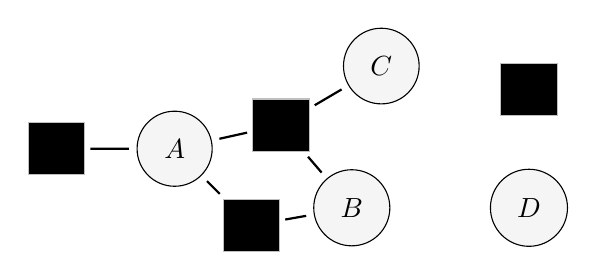
\begin{tikzpicture}[scale=0.75]					
				\node[fgnode] (A) at (0, 0) {$A$};
				\node[fgnode] (B) at (3, -1) {$B$};
				\node[fgnode] (C) at (3.5, 1.4) {$C$};
				\node[fgnode] (D) at (6, -1) {$D$};
				
				
				
				\node[factor] (f1) at (-2, 0){$\phi_1$};
				\node[factor] (f2) at (1.8,.4){$\phi_2$};
				\node[factor] (f3) at (1.3, -1.3){$\phi_3$};
				\node[factor] (f4) at (6, 1){$\phi_4$};
				
				
				\draw[thick] (f1) -- (A) -- (f2) -- (B) -- (f3) -- (A);
				\draw[thick] (C) -- (f2);
		\end{tikzpicture} }
		\caption{Factor Graph: exam scores}
		\label{fig:fg-exam}
	\end{figure}
	
	
	\begin{enumerate}[nosep]
%joe4
			  %		\item[$\phi_1$.] A. priori., Alice is 4 times
%                  as likely to pass as not, and so $\phi_1(a)
	\item[$\phi_1$.] \emph{A priori}, Alice is 4 times
			  as likely to pass as not, so $\phi_1(a)
					  = 4$ if $a = 1$, and 1 otherwise. 
\item[$\phi_2$.] Alice, Bob, and Clara
					  collaborated. Clara is very persuasive, and
					  Alice trusts her, so an outcome in which
					  everyone gets the same score is (a priori) 8 times more
%joe4: more likely than what?  One where they don't all get the same
%score?  If so, then Alice and Clara getting the same score can't be 4
%times more likely than them getting different scores.  I'm confused
%oli5: we discussed this in our meeting, but the correct interpetation is via energies. The relative likelihood holds locally and works if it doesn't interat with other factors---but the one I'm presenting is the only analogy to local graphical models we have.
%oli5: addressing "more likely than what"--added                          
					  likely than when each score is distinct,
%   
					  one in which only Alice and Clara
					  share a score is 4 times as likely, and one
					  in which only Bob and Clara share a score is
					  twice as likely. 
		\[ \phi_2(a,b,c) = \left\{\begin{aligned}
%joe4: redid layout to make it more standard
%oli5: That was a premature optimization to save space on my part, but this example is too bulky to make it into the short paper anyway.
			  %			8 &~~ \text{if~} a = b = c; 
						8 &~~ \text{if~} a = b = c;\\
									4 &~~ \text{if~}c = a \neq b; \\
			2 &~~ \text{if~}c = b \neq a;\\
			1 &~~ \text{otherwise.}
		\end{aligned}\right. \]
%joe4*: This seems inconsistent with the claim above that they're all
%more like to get the same score as not.  If this is intentional, you
%need to say someting about it.
%oli5: Perhaps I should do a better job of this earlier, but I describe below.
%joe5: I'm not reading that carefully at this point, because I
%currently think that this is the wrong story.
		  \item[$\phi_3$.] Alice thinks very poorly of
					  Bob, and ultimately reverses the answers to
					  all his questions; she's guarantee to fail
					  if he passes, and vice versa. $\phi_3(a,b) =
					  1$ if $a \neq b$ and 0 if $a=b$.
			%oli5: added. 
					  Note that this is
											  incompatible with
											  $\phi_2$, and so the
											  factor graph cannot
											  satisfy both
											  constraints
											  exactly. 
%joe4: I don't undersatnd the meaning of the isolated box \phi_4.  
%oli5: It's just a factor connected to zero variables. It has a value,
%but doesn't matter. Part of the point is that factor graphs encode a
%lot of useless information.
%joe5: If that's the point, you need to make it.
											\item[$\phi_4$.] The test is on factor graphs, which was unlikely, so $\phi_4() = 0.25$. This is true independent of anyone's scores, and doesn't bear on the distribution, so it will get normalized out.
	\end{enumerate}
	We don't know anything about David. The resulting distribution is given in \Cref{tab:fg-exam-dist}
	
	\begin{table}[h!]
		\renewcommand{\arraystretch}{1.15} 
		\centering
		\begin{tabular}{c|cc|cc}
			\multicolumn{1}{c}{}&\multicolumn{2}{c}{$a_0$} & \multicolumn{2}{c}{$a_1$} \\[-0.3em]
			&$c_0$ & $c_1$ & $c_0$ & $c_1$ \\\hline
			$b_0$&0 & 0 & .2667 & .5333 \\
			$b_1$&.1333 & .0667 & 0 & 0
		\end{tabular}
		
		\caption{The resulting distribution from \Cref{ex:fg-exam}}
		\label{tab:fg-exam-dist}
	\end{table}
	
	
	Note some features of this example:
	\begin{enumerate}[nosep]
%joe4: this should be mntion earlier (when you define \phi_3)
%joe4: this too should be mentioned earlier.  I noted it and was onfused.
%oli5: done.
			\item $\phi_3$ totally overrides the first case of $\phi_2$: The
directions of an individual factor are just suggestions that are
resolved globally. 
		%The intuition of relative likelihoods, only works locally.
\item Although $\phi_3$ was symmetric, our
					  story is not: Alice doesn't trust Bob, and
					  not the other way around. There is an
					  important distinction in the story (this
					  changes Alice's score, and not Bob's), but
					  this cannot be captured. 
%			To capture a conditional probability distributions, you need to impose \emph{local} normalization constraints \cite{frey2012extending}. In this case, this means insisting that  $\sum_{a} \phi_3(a,b) = 1$
		\item To get any marginal distribution such as $\Pr(B)$, you have to take into account every factor, including those such as $\phi_1$ that are not connected to $B$.
		\item To emphasize that a factor is more important, we cannot simply scale it, as the scaling will be normalized out; the only control available is to changing the variance of its items: setting things (close to) zero is the only way to ensure that the factor matters more than others.
	\end{enumerate}
\end{example}
%joe4: this may be true, but it's irrelevant        
%	Generally, factor graphs are learned from data or translated
%        from another model, rather than specified by
	%        hand.  \Cref{ex:fg-exam} should make it clear why: there is a
As \Cref{ex:fg-exam} shows, there is a lot of freedom in specifying the factors, 
%oli5: added
and very little in the way of locally interpretable semantics. 


\subsection{DIRECTED FACTOR GRAPHS}

One solution, by \cite{frey2012extending} is to also enforce some local constraints, in the form of a local normalization.  While this indeed solves issues \cref{fgproblem:undirected,fgproblem:global}, directed factor graphs still leave some bits of issues \cref{%fgproblem:corrob,
	fgproblem:reweight,fgproblem:volatile} unaddressed.

Directed factor graphs are much more explicit with their factorizations than BNs, are as expected, even more closely related to PDGs. However, they too cannot capture scenarios such as \cref{ex:randomvars}. Consider example \ref{ex:directedfg}

\begin{example}\label{ex:directedfg}
	\todo{Choose a different directed factor graph example that doesn't rely on sub-stochasticity}
\end{example}





\section{Structure-editing PDG Operations}

While both PDGs and PDH s are equivalent, and despite the fact that dealing with sets of variables is standard, we chose PDGs over PDH s as the face of the paper. One of the primary reasons to do this is that it puts products on equal footing with other equally valid structural modifications we could have done instead, rather than specializing the definitions for products.

\begin{enumerate}
	\item Latent variable nodes, e.g., through VAEs. Useful for representation learning and modeling bounded agents that just remember the gists of things.
	
	\item Sums nodes. For when one is being forced to chose between two options which might otherwise be unrelated, and the basic constructor for variables from points.
	
	\item Exponential nodes. Any positive temperature arrow can be reasoned about through expansion into its parameters.
	
	\item Compression nodes: e.g., truncation nodes for propositions. It may not matter exactly what proof you have so long as you've proved one exists. That a variable takes a value may be just as important as it.
\end{enumerate}


\section{More Examples}\label{sec:more-examples}

\begin{example}
	\label{ex:corrob}
\end{example}

\begin{example}[Maximum Entropy with cpds is not the BN distribution]\label{ex:counterexample}
	Consider the Bayesian network 
	\begin{tikzcd}[cramped, sep=small]
		A \ar[r] & C & B \ar[l]
	\end{tikzcd}
	where $A$ and $B$ are binary, and $C$ can take $2^k$ values, including $c_0$. We now give the associated tables: both $A$ and $B$ get prior unconditional probabilities of $\nicefrac12$ apiece, and set $C$'s cpd to be
	\[
		\begin{idxmat}{{$a$,$b$},{$\bar a$, $b$},{$a$, $\bar b$},{$\bar a$, $\bar b$}}{$\Delta C$}
			\mathit{Uniform} \\ \delta_{c,c_0 }\\ \delta_{c,c_0} \\ \mathit{Uniform} \\
		\end{idxmat}
	\]
	where $\delta_{c,c_0}$ is the degenerate distribution that puts all mass on $c_0$. Looking at entropy, the uniform distribution on $C$ gets $k$ bits, and each of $A$ and $B$ we know each give one bit. 
	The semantics of a BN require that $A$ and $B$ are independent, since neither is a descendent of the other and neither has parents.  However, doing so results in a distribution of entropy $H(p) = 2 + k/2$ (one for each of the independent bits, and an expected k/2 bits from getting the uniform distribution on $C$ half the time), whereas if we correlate $A$ and $B$ so that they are always equal, we get $1 + k$ bits, one total bit from $A$ and $B$, and $k$ from $C | A,B$. For any finite $k$, this is still not the maximum entropy distribution, but it is much higher entropy than the one the BN suggests.
	
	Therefore the maximum entropy distribution consistent with the tables does not encode the independece assumption that a BN does. 
\end{example}

\begin{example}\label{ex:randomvars}
	Consider random variables $X_1$, $X_2$  on a set
			$\Omega$ of outcomes (distributed according to $p$),
			taking values in the set $\mathcal X$. This can be
			represented as the PDG below. 
	\begin{center}
		\scalebox{0.8}{
			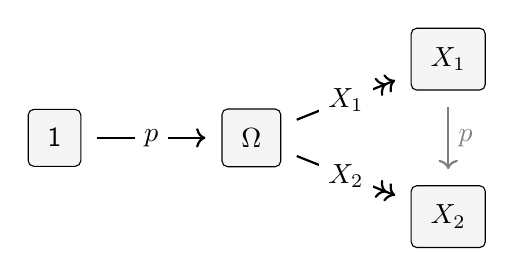
\begin{tikzpicture}
			\node[dpadded] (1) at (0,0) {$\sf 1$};
			\node[dpadded] (W) at (2.5,0) {$\Omega$};
			\node[dpadded] (X1) at (5,1) {$X_1$};
			\node[dpadded] (X2) at (5,-1) {$X_2$};
			
			\draw[arr] (1) to node[fill=white]{$p$} (W);
			\draw[arr, ->>] (W) to node[fill=white]{$X_1$} (X1);
			\draw[arr, ->>] (W) to node[fill=white]{$X_2$} (X2);
			\draw[arr, gray] (X1) to node[right] {$p$} (X2);
			\end{tikzpicture}}
	\end{center}
	The setup so far, in black above, can be captured with a BN, but it is impossible to also articulate conditional probabilistic relations amongst the variables in the same time: in a BN, once we add a variable $\Omega$ which caracterizes all possible worlds as a parent of a variable (e.g., $X_2$), any other dependences will be irrelevant. Given a world $\omega$ and values of other variables, the cpd associated to $X_2$ would simply deterministically return the value of $X_2$ in $\omega$. 
	
	As a result, a BN has to choose between encoding conditional probabilistic information, and the knowledge of the complete information from $\Omega$. This is not true with a PDG, which makes it possible to simultaneously model the structure of the random variables around an agent's beliefs, in addition to the beliefs themselves.
\end{example}


\begin{vcat}
	\section{Categorical Presentation}
	\note{I will not put any time into this, as it's not going in the paper, but it's here as a placeholder, and I'll list some reasons why this is worth thinking about.}
	One reason this works out so nicely is every construction is universal. We can in fact give a simpler categorical presentation of PDGs for those who already know category theory. The highlights are as follows:
	\begin{enumerate}
		\item A PDG is an attention-shaped diagram in the Markov category. That is, functor from the free category generated by the graph $(\mathcal N, \Ed)$ representing attention, to the Markov category. Indeed $\mathcal V$ is the action on objects, assigning each $\mathcal N$ to a measurable set, $\mat p$ is the action on morphisms, sending edges in $\Ed$ to Markov kernels between their associated objects. 
		\begin{enumerate}
			\item Composition works out in general as we place no restrictions on anything, but
			\item If every edge in $\Ed$ represents the causal structure of their relationship, then the image of the resulting diagram will be flat, and so effectively there will only be at most one, belief, and no possibility of conflict.
			\item Interpreting with a different model of uncertainty (such as the powerset, giving us non-deterministic possibility) is simply an exchange of interpretation. However, for nice interaction with deterministic functions and logic, this notion of uncertainty must be a monad.
		\end{enumerate}
		
		\item This highlights the role of the ``qualitative'' and ``quantitative'' versions of this framework (which work out much more cleanly than for BNs in a categorical sense)
		
		\item A limit of this diagram is a space of worlds and all of the random variables as functions. A colimit is a the strongest thing that must be true according to the model (suspicion: this is somehow related to common knowledge). There is some strangeness about how samples work that I have not yet figured out.
	\end{enumerate}
	
	
	\section{Algebra}\label{sec:algebra}
	\begin{defn}
		If $\sigma$ is a signature, a $\sigma$-PDG $M'$ on a PDG $M=(\mathcal N, \Ed, \mathcal V, \mu)$ is a \modelname\ $(\mathcal N', \Ed', \mathcal V', \mu')$ such that
		\begin{itemize}
			\item $\mathcal N':= T_\sigma(\mathcal N)$ is the term algebra for the signature $\sigma$ over the alphabet $\Sigma = \mathcal N$.
			\item $\Ed' = \Ed \cup \Ed^\sigma$ is $\Ed$ extended with extra edges for operations that are 
		\end{itemize}
	\end{defn}
	
	\begin{example}
		content
	\end{example}		
\end{vcat}

}
%joe7: \end{commentout}
% \end{notfocus}

\section{Proofs} \label{sec:proofs}
%oli10: added this subsection and reorganized propositions /
%definitions accordingly.i
	%joe9: removed section
%	\subsection{Standard Definitions and General Facts}
%joe9: let's be consistent and write \mu for the default distribution
%	For brevity, we use the standard notation and write $p(x, y)$
%        instead of $p(X \!=\! x, Y \!=\! y)$, $p(x \mid y)$ instead of
	%        $p(X \!=\! x\mid Y \!=\! y)$, and so forth.
		For brevity, we use the standard notation and write $\mu(x, y)$
	instead of $\mu(X \!=\! x, Y \!=\! y)$, $\mu(x \mid y)$ instead of
	$\mu(X \!=\! x\mid Y \!=\! y)$, and so forth.
%joe9: I don't understand this
%        So long as $x$ is bound solely as an element of $\V(X)$, the
%        meaning is unambiguous.  

	%joe9: this should go where we use it; I put it there
	\commentout{
\begin{defn}[Conditional Entropy]
	If $p$ is a distribution over a set $\Omega$ of out comes, and $X$ and $Y$ are random variables on $\Omega$, then the \emph{conditional entropy}, $\H_p(X \mid Y)$, is defined as 

\end{defn}

%joe9*: I think we shoul cut this; we don't need it.
	\begin{defn}[Sets as Variables] \label{def:set-rv}
	Sets of random variables as random variables. If $S$ is a set of random variables $X_i : \Omega \to \V(X_i)$ on the same set of outcomes $\Omega$, we consider $S$ itself to be the random variable taking values $\V(X) = \{(x_1, \ldots, x_i \ldots) \}$ for $x_i \in \V(X_i)$. Formally, we define its value on a world $\omega$ to be $S(\omega) := (X_1(\omega), \ldots, X_i(\omega), \ldots)$. 
\end{defn}

%joe9*: I think we should cut this; we don't need it.  We need strict
%convexity, which has a much simpler definition.                
%oli10: added
\begin{defn}[Strong Convexity] \label{def:strong-convexity}
	A real-valued function is $m$-\emph{strongly convex}, if there is a quadratic lower bound, with coefficient $m$, away from its first order approximation. More precisely, it is $m$ strongly convex if for every $x, y$ in its domain, 
	\[ f(y) \geq f(x) + \Big\langle\nabla f(x), y-x \Big\rangle + m\norm{x-y}^2_2 \]
\end{defn}

%joe9*: we should cut this; it's doubtless a standard reslt, and we
%don't need it.
%oli11: I actually asked Bobby for a reference and he said it was so
%standard that everyone just says it. He even looked through a couple
%standard convex analysis books and says it's not there. I proved it
%because you asked for a result I couldn't find one. 
%oli11: It may be worth keeping some of the strong convexity stuff
%around though; strong convexity is a _lot_ more useful for finding
%the minimum than strict convexity, and ML people will immediately
	%know that this means it is efficient.
%joe10: NO!  Don't clutter up the paper with things ou don't need!
	%This is bad style!
\begin{prop}\label{prop:neg-ent-convex}
%joe8*: you can't pull 1-strong convexity out of a hat, and define it
%in the proof.  You need to define it, and explain why you care.  Your
%proof also looks at hte function xlog x, so whynot state the
%proposition in terms of that?
%oli10: definition added above
  Negative entropy, restricted to a finite probability
			simplex, is 1-strongly convex. 
\end{prop}
\begin{proof}
	%https://math.stackexchange.com/questions/3077287/how-to-show-negative-entropy-function-fx-x-logx-is-strongly-convex
	Let $X$ be a finite set; the function $f: \Delta(X) \to \mathbb R$ given by $\vec x \mapsto \sum x_i \log x_i$ is strongly convex, as 
	\begin{equation*}
		\partial_j f(\vec x) =  \partial_j\left[\sum_i x_i \log x_i \right] = 
			x_j \partial_j \big[\log x_j \big] + \log x_j = 1 + \log x_j
	\end{equation*}
	So
	\begin{align*}
		\Big\langle \nabla f(x) - \nabla f(y),~ x-y\Big\rangle 
			&= \sum_i \Big((\partial_i f)(\vec x) - (\partial_i f)(\vec y)\Big)(x_i - y_i) \\
			&= \sum_i \Big(\log x_i  - \log y_i \Big)(x_i - y_i) \\
			% &= \sum_i x_i \log x_i + y_i \log y_i + 2 
		\intertext{As $\log$ is concave, we have $\log(y_i) \leq \log(x_i) + (y_i-x_i) \frac{\mathrm d}{\mathrm d x_i} [\log(x_i)]$, and so $\log x_i - \log y_i \geq (1/x) (x - y)  \geq (x-y)$, we have}
		\Big\langle \nabla f(x) - \nabla f(y),~ x-y\Big\rangle
			&= \sum_i \Big(\log x_i  - \log y_i \Big)(x_i - y_i) \\ % from above
			&\geq \sum_i (x_i-y_i)^2 \cdot \frac1{x_i}\\
			&\geq \sum_i (x_i-y_i)^2 \\
			&= \norm{x-y}^2_2 \numberthis\label{proofeqn:strong1}
%joe9: When I latex this, I get the error ``You can't use `\halign' in
%math mode.''  (I've gotten this error all along; it's nothing new.) 
%oli11*: only in aligns that have a \numberthis, or all align environments?
% we should fix this...
%joe10: I'm not sure; I didn't check.  I shouldn't have to spend time
%doing thi!
	\end{align*}
	At the same time, the condition for convexity can be phrased in terms of gradients as the condition that for all $x,y$,
	\[  \Big\langle \nabla f(x) - \nabla f(y),~ x-y\Big\rangle \geq 0\]
	So together with \eqref{proofeqn:strong1}, we conclude that the function $f - \norm{x-y}^2_2$ is convex. Therefore, $f$ is 1-strongly convex.
\end{proof}

	}
%joe9: \end{commentout}
	
\subsection{Properties of Scoring Semantics}

%joe17*: If we use this theorem somewhere, it can stay.  But if not,
%we should cut it.  We should only include results we need.  Also,
%when I latex this, the theorem statement is missing.
%oli20: Yeah, this is a special case of another theorem, and we don't need it. 
% only useful as a property of the first semantics one might keep in mind.
\vleftovers{
	\thmsetconvex*
	\begin{proof}
		Choose any two distributions $p, q \in \SD{M}$ consistent with $M$, any mixture coefficient $\alpha \in [0,1]$, and any edge $(A,B) \in \Ed$.

		By the definition of $\SD{M}$, we have $p(B = b \mid A = a) = q(B = b \mid A = a) = \bmu_{A,B}(a,b)$.  
		For brevity,j we will use little letters ($a$) in place of events ($A = a$).
		Therefore, $p(a\land b) = \bmu_{A,B}(a,b) p(a)$ and $q(ab) = \bmu_{A,B}(a,b) q(a)$. Some algebra reveals:
		\begin{align*}
			\Big( \alpha p + (1-\alpha) q \Big) (B = b \mid A = a) &= 
			\frac{\Big( \alpha p + (1-\alpha) q \Big) (b \land a)}{\Big( \alpha p + (1-\alpha) q \Big) (a)} \\
			&= \frac{ \alpha p(b \land a) + (1-\alpha) q(b \land a) }{\Big( \alpha p(a) + (1-\alpha) q (a)} \\
			&= \frac{ \alpha \bmu_{A,B}(a,b) p(a) + (1-\alpha) \bmu_{A,B}(a,b) q(a) }{\Big( \alpha p(a) + (1-\alpha) q (a)} \\
			&=\bmu_{A,B}(a,b) \left(\frac{ \alpha  p(a) + (1-\alpha) q(a) }{\Big( \alpha p(a) + (1-\alpha) q (a)}\right)\\
			&= \bmu_{A,B}(a,b)
		\end{align*}
		and so the mixture $\Big(\alpha p + (1-\alpha) q \Big)$ is also contained in $\SD{M}$.
	\end{proof}
}
%joe9: just because it's n appendix, it doesn't mean that we shouldn't
%tell a story.
%joe17: If we keep the previous result, this should go above it
In this section, we prove the properties of scoring functions that we
mentioned in the main text,
Propositions~\ref{prop:sd-is-zeroset}, \ref{prop:sem3}, and
\ref{prop:consist}.  We repeat the statements for the reader's convenience.

%joe9: put this first
%	\begin{prop}\label{prop:sd-is-zeroset}
%oli15: consistency
% \begin{old}{prop:sd-is-zeroset}
% 	For any PDG $\dg M$, $\SD{\dg M} = \{ \mu : \bbr{\dg M}_0(\mu) = 0\}$. 
% \end{old}
% \recall{prop:sd-is-zeroset}
\restate{prop:sd-is-zeroset}{
$\SD{\dg M} \!= \{ \mu : \bbr{\dg M}_0(\mu) \!=\! 0\}$ for all $\dg M$.
}
\begin{proof}
	 By taking $\gamma = 0$, the score is just $\Inc$. By
%joe9
%                 definition, any $\mu \in \SD{\dg M}$ satisfies all
%                 constraints, hence satisfies $\mu(Y \mid X=x) =
%                 \bp(x)$ for any $L \in \Ed^{\dg M}$ and $x$ with
%                 \bp(x)$ for any $L \in \Ed^{\dg M}$ and $x$ with
			 definition, a distribution $\mu \in \SD{\dg M}$ satisfies
	  all the
			 constraints, so $\mu(Y = \cdot \mid X=x) =
			 \bp(x)$ for all edges $X \rightarrow Y \in \Ed^{\dg
			   M}$ and $x$ with 
%joe9*: this needs a reference
%oli11
			 % $\mu(X=x)>0$. By Gibbs inequality,
			 $\mu(X=x)>0$. By Gibbs inequality
			 \cite{mackay2003information}, 
			 $\kldiv{\mu(Y|x)}{\bp(x)} = 0$. Since this is true
			 for all edges, we must have $\Inc_{\dg M}( \mu) =
			 0$. Conversely, if $\mu \notin \SD{\dg M}$, then it
			 fails to marginalize to the cpd $\bp$ on some edge
%joe9
			 %                 $L$, and so again by Gibbs inequality
							  $L$, and so again by Gibbs inequality,
			 $\kldiv{\mu(Y|x)}{\bp(x)} > 0$. As relative entropy
			 is non-negative, the sum of these terms over all
			 edges must be positive as well, and so $\Inc_{\dg M}(
			 \mu) \neq 0$. %This is true whether or not $\dg M$ is
						   %consistent. 
\end{proof}


%joe9
Before proving the remaining results, we prove a lemma that will be useful
in other contexts as well. 

%oli11: aaahhh it took me an hour to edit this, and I don't think
%anything even changed. 
% Why did you modify it? It was so much cleaner before.
%joe10: I thought it was overkill ... 
\begin{lemma}
	% [name=\Cref{prop:convex} analog, 	restate=thmincconvex]
	\label{thm:inc-convex}
	$\Inc_{\dg M}( \mu)$ is a convex function of $\mu$.
\end{lemma}
\begin{proof}
%joe14: you need a reference for this
%oli16: I could not find it in MacKay, but it is in Cover and Thomas'
%"Elements of Information Theory". Citation added. 
  %  It is well-known that $\thickD$ is convex, in the sense that
    It is well known that $\thickD$ is convex \cite[Theorem
%joe15: for what it's worth, this was already in joe.bib.  I'm using
%that version, since it corrects some problems in your reference
%(e.g., book titles should be capitalized)
      %      2.7.2]{cover2012elements}, in the sense that
            2.7.2]{coverThomas}, in the sense that  
	\[ \kldiv{\lambda q_1 + (1-\lambda) q_2 }{ \lambda p_1
			  + (1-\lambda) p_2} \leq \lambda \kldiv {q_1}{ p_1} +
%joe9
			%                (1-\lambda) \kldiv{q_2}{p_2} \]
							(1-\lambda) \kldiv{q_2}{p_2}. \] 
%joe9
%		Choose any edge $L \in \Ed$ from $A$ to $B$, and also
			%                any $a \in \mathcal V(A)$.
Given an edge $L \in \Ed$ from $A$ to $B$ and $a \in \mathcal V(A)$,
and   
%oli11
% etting $q_1 = q_2 = \bp(a)$, we get that
setting $q_1 = q_2 = \bp(a)$, we get that
	\[ \thickD(\bp(a) \ ||\ \lambda p_1 + (1-\lambda) p_2)
			\leq \lambda \thickD (\bp(a) \ ||\ p_1) + (1-\lambda)
%joe9
			%                \thickD(\bp(a)\ ||\ p_2) \]
							\thickD(\bp(a)\ ||\ p_2). \] 
	Since this is true for every $a$ and edge, we can take
		   a weighted sum of these inequalities for each $a$
%joe9
		   %               weighted by $p(A=a)$, and therefore
		   weighted by $p(A=a)$; thus, 
%oli11: I think the NeurIPS style guide wants us to avoid
% the TeX primitive $$, in favor of \[, as this behavior can be styled, while the TeX primitve cannot. 
	\begin{align*}
		\Ex_{a\sim p_A} \kldiv{\bp(a)}{\lambda p_1 +
			(1-\lambda) p_2} &\leq 
			 \Ex_{a\sim p_A}\lambda \kldiv {\bp(a)}{p_1} +
											(1-\lambda)
%joe14
                         %			 \kldiv{\bp(a)}{p_2} \\
                         			 \kldiv{\bp(a)}{p_2}. \\
%oli11: the next line does what you added; I'm adding more
% \intertext{and}
%joe14
                        \intertext{Taking a sum over all edges, we get
                        that}
					\sum_{(A, B) \in \Ed}\mskip-10mu\Ex_{a\sim p_A} \kldiv{\bp(a) }{\lambda p_1 + (1-\lambda) p_2} 
			&\leq \sum_{(A, B) \in
							  \Ed}\mskip-10mu\Ex_{a\sim p_A}\lambda
							\kldiv{\bp(a)}{p_1} + (1-\lambda)
%joe14
%							\kldiv{\bp(a)}{p_2} \\
							\kldiv{\bp(a)}{p_2}. \\
		                                        %joe9
%oli11: reinstated intertext and deleted ``$$ and $$''
%oli11 removing "and so" breaks flow of equantions; replace with \implies
		% \intertext{and so,}
%joe14: you shuld use the logical implication symbol in the middle of a proof
%like this.
%oli16: I assume you meant to say "should not". Why is that? The
%symbol is universal, and the words break up the alignment of the
%equations, which helps 
% me see visually what changes were made. The words are also longer,
%causing a more 
% spread-out proof; the words themselves do not carry any extra meaning. It also
% visually simplifies the proof, and I put enough space and use the long versions,
% (instead of \Rightarrow / \Leftarrow), which are very rarely used as formal
% connectives in a language. In any case, this is not even a setting where 
% there could be any confusion between semantics and syntax. 
%
% This is likely to be a place where we have differing sensibilities. I would
% like to be convinced that your way of doing things is better, but as you can
% see, I have a lot of reasons that I dislike this stylistically. Do you have an
% argument that you think could persuade me? If not, the resulting compromise
% below might be the worst of both worlds (display mode equations that you are
% not a fan of, broken up with text in a way that reduces the visual benefit of
% displaymode equations for me, and expands the proof in a way that neither of
% us are happy with).
%joe15: I typically reserve logical symbols for logical expressions.
%It is fairly standard rule, although I'm not going to hunt down a
%reference.  I actully found it hard to distinguish the logical =>
%from the equations, so it made things worse for me.
%oli16: In any case, I'm updating  your change so that it displays
%properly with an intertext. I'm  
% not sure why you don't like "intertext" in general, but perhaps
%\shortintertext 
% gives you what you're looking for?
%joe15: I've never used \interext.  My concern is that it encourages
%you to write a lot of math (equations interspersed with a bit of
%text) rather than English.  I'm also getting lots of latex errors
%that I don't know how to fix.    
    \shortintertext{It follows that} 
%       It follows that
  %                         \implies\qquad
		\Inc_{\dg M}( \lambda p_1) + (1-\lambda)p_2)
%joe9
%                        &\leq \lambda \Inc_{\dg M}(p_1) + (1-\lambda)
					%                        \Inc}{\dg M}(p_2)
%oli11: inserted missing alignment character
					&\leq \lambda \Inc_{\dg M}(p_1) + (1-\lambda)
					\Inc_{\dg M}(p_2). 
											%joe9
%joe16: I still get a latex error here
	\end{align*}
%		Therefore $\Inc_{\dg M}( \mu)$ is a convex function of $\mu$
%oli11:
% I'm still not sure why you even re-structured the TeX of this proof, but it confused my editor. 
	Therefore, $\Inc_{\dg M}( \mu)$ is a convex function of $\mu$.
\end{proof}

%joe9: added glue
The next proposition gives us a useful representation of $\bbr{M}_\gamma$.
\restate{prop:nice-score}{
Letting $x^{\mat w}$ and $y^{\mat w}$ denote the values of
 $X$ and $Y$, respectively, in $\mat w \in \V(\dg M)$, 
we have 
\begin{equation*}
\begin{split}
\bbr{\dg M}(\mu) =  \Ex_{\mat w \sim \mu}\! \Bigg\{
% \bbr{\dg M}(\mu) =  \!\!\!\sum_{\mat w \in \V(\dg M)} \!\!\! \mu(\mat w) \Bigg\{
\sum_{ X \xrightarrow{\!\!L} Y  }
\bigg[\,
%oli26: removing annotations
% \color{gray} \overbrace{\color{black}
	 \!\beta_L \log \frac{1}{\bp(y^{\mat w} |x^{\mat w})}
%oli26
   % }^{\color{gray}\smash{\mathclap{\text{log likelihood / cross entropy}}}} 
%oli26: remove line split
% + \\[-0.5em]
   +
%oli26:
   % \color{gray}\underbrace{\color{black} 
(\valpha{\alpha_L}\gamma - \beta_L ) \log \frac{1}{\mu(y^{\mat w} |x^{\mat w})} 
%oli26:
 %  }_{\color{gray}\smash{\mathclap{\text{local regularization (if $\beta_L > \gamma$)}}}}
 \bigg] - 
%oli26
 % \underbrace{\color{black}
	\gamma \log \frac{1}{\mu(\mat w)}
   % }_{\color{gray}\smash{\mathclap{\text{global regularization}}}}\color{black} 
   \Bigg\} .
\end{split}
\end{equation*}
}
\begin{proof}
%oli26: added
We use the more general formulation of $\IDef{}$ given in \Cref{sec:expfam}, in which each edge $L$'s conditional 
information is weighted by $\alpha_L$.
  \begin{align*}
	\bbr{\dg M}_\gamma(\mu) &:= \Inc_{\dg M}( \mu) + \gamma \IDef{\dg M}(\mu) \\
		% Next, replace expressions for Inc and Extra
		&= \left[\sum\alle \beta_L \Ex_{x\sim \mu_X}\kldiv[\Big]{ \mu(Y | X \sheq x) }{\bp(x) } \right]  + \gamma \left[\sum\alle \alpha_L \H_\mu(Y\mid X) ~-\H(\mu)\right]\\
		% Combine the summations and expectations
		&= \sum\alle 
			\Ex_{x \sim \mu_{\!_X}}  \left[ \beta_L\; \kldiv[\Big]{ \mu(Y \mid x) }{\bp(Y \mid x) } + \gamma \; \alpha_L \H(Y \mid X\sheq x) \right]  - \gamma \H(\mu) \\ 
		% Now, Expand relative and conditional entropy
		&= \sum\alle 
			\Ex_{x \sim \mu_{\!_X}}  \left[ \beta_L\; \left(\sum_{y \in \V(Y)} \mu(y \mid x) \log\frac{\mu(y\mid x)}{\bp(y\mid x)}\right) + \alpha_L\gamma \; \left(\sum_{y \in \V(Y)} \mu(y\mid x) \log \frac{1}{\mu(y\mid x)} \right) \right]  - \gamma  \H(\mu) \\ 
		%combine common \sum \mu(y | x) 
		&= \sum\alle 
			\Ex_{x \sim \mu_{\!_X}}  \left[ \sum_{y \in \V(Y)} \mu(y \mid x) \left(  \beta_L\; \log\frac{\mu(y\mid x)}{\bp(y\mid x)} + \alpha_L \gamma \; \log \frac{1}{\mu(y\mid x)} \right) \right]  - \gamma  \H(\mu) \\
		% Expand entropy and reduce sum to expectation
		&= \sum\alle 
			\Ex_{x \sim \mu_{\!_X}}  \left[ \Ex_{y \sim \mu(Y \mid X=x)} \left(  \beta_L\; \log\frac{\mu(y\mid x)}{\bp(y\mid x)} + \alpha_L \gamma \; \log \frac{1}{\mu(y\mid x)} \right) \right]  - \gamma \sum_{\mat w \in \V(\dg M)} \mu(\mat w) \log \frac{1}{\mu(\mat w)} \\  
		% combine expectation.
		&= \sum\alle 
			\Ex_{x,y \sim \mu_{\!_{XY}}}  \left[ \beta_L\; \log\frac{\mu(y\mid x)}{\bp(y\mid x)} + \alpha_L\gamma \; \log \frac{1}{\mu(y\mid x)}  \right]  - \gamma  \Ex_{\mat w \sim \mu} \left[ \log \frac{1}{\mu(\mat w)}\right] \\
		% swap sum and expectation, and use log rule to split kl divergence
		&= \Ex_{\mat w \sim \mu} \Bigg\{   \sum_{ X \xrightarrow{\!\!L} Y  } \left[
			\beta_L \log \frac{1}{\bp(y\mid x)}   - \beta_L  \log \frac{1}{\mu(y \mid x)}+ \alpha_L\gamma \log \frac{1}{\mu(y \mid x)} \right]\Bigg\}  -  \gamma  \Ex_{\mat w \sim \mu} \left[\log \frac{1}{\mu(\mat w)}\right] \\
		% combine
		&=  \Ex_{\mat w \sim \mu} \Bigg\{ \sum_{ X \xrightarrow{\!\!L} Y  } \left[
			\beta_L \log \frac{1}{\bp(y\mid x)} +
	                        (\alpha_L\gamma - \beta_L ) \log
	                        \frac{1}{\mu(y \mid x)} \right] -
	                        \gamma \log \frac{1}{\mu(\mat w)}  \Bigg\}.  
	\end{align*}
\end{proof}

	%joe9
%        	\begin{prop} \label{prop:convex-if-gamma-small}
%	  For a PDG $\dg M$, and any $\gamma$ such that $0 <
%          \gamma \leq \min_L \beta_L^{\dg M}$, then $\bbr{\dg
%          If $\dg M$ is a PDG and   $0 < \gamma < \min_L \beta_L^{\dg M}$, then
%          then $\bbr{\dg
%                  M}_\gamma$ is a strictly convex function of $\mu$.
%	\end{prop}
We can now prove         Proposition~\ref{prop:sem3}.
% \begin{old}{prop:sem3}
% If $\dg M$ is a PDG and
% $0 < \gamma
% \leq \min_L \beta_L^{\dg M}$, then
% $\bbr{\dg M}_\gamma^*$ is a singleton.
% \end{old}
\restate{prop:sem3}{
If $\dg M$ is a PDG and $0 < \gamma \leq \min_L \nicefrac{\beta_L^{\dg M}}{\alpha_L^{\dg M}}$, then
$\bbr{\dg M}_\gamma^*$ is a singleton. 
}
\begin{proof}
	  %joe9:
It suffices to show that $\bbr{\dg
			  M}_\gamma$ is a strictly convex function of $\mu$,
since every strictly convex function has a unique minimum.
%joe9
%We can rewrite the semantics as
Note that
%oli22: added \alpha to proofs
\begin{align*}
\bbr{M}_\gamma(\mu) 
	&= \Ex_{\mat w \sim \mu} \Bigg\{   \sum_{ X \xrightarrow{\!\!L} Y  } \left[
		\beta_L \log \frac{1}{\bp(y\mid x)} + (\valpha{\alpha_L}\gamma - \beta_L ) \log \frac{1}{\mu(y \mid x)} \right] - \gamma \log \frac{1}{\mu(\mat w)} \Bigg\} \\
	&= \Ex_{\mat w \sim \mu} \Bigg\{   \sum_{ X \xrightarrow{\!\!L} Y  } \left[ \gamma \valpha{\alpha_L} \log \frac{1}{\bp(y\mid x)} + 
		(\beta_L - \valpha{\alpha_L} \gamma) \log \frac{1}{\bp(y\mid x)} - (\beta_L - \valpha{\alpha_L} \gamma) \log \frac{1}{\mu(y \mid x)} \right] - \gamma \log \frac{1}{\mu(\mat w)} \Bigg\}  \\
	&= \Ex_{\mat w \sim \mu} \Bigg\{   \sum_{ X \xrightarrow{\!\!L} Y  } \left[ \gamma \valpha{\alpha_L} \log \frac{1}{\bp(y\mid x)} + 
		(\beta_L - \valpha{\alpha_L} \gamma) \log \frac{\mu(y\mid x)}{\bp(y\mid x)} \right] - \gamma \log \frac{1}{\mu(\mat w)} \Bigg\} \\
	&=  \sum_{ X \xrightarrow{\!\!L} Y  } \left[ \gamma \valpha{\alpha_L} \Ex_{x,y \sim \mu_{\!_{XY}}} \left[ \log \frac{1}{\bp(y\mid x)} \right] + 
		(\beta_L - \valpha{\alpha_L} \gamma) \Ex_{x\sim\mu_X}
          \kldiv[\Big]{\mu(Y\mid x)}{\bp( x)} \right] - \gamma \H(\mu). 
\end{align*}
	The first term, 
	\( \Ex_{x,y \sim \mu_{\!_{XY}}} \left[-\log {\bp(y\mid x)}\right] \) 
	is linear in $\mu$, as $\bp(y\mid x)$ does not depend on $\mu$. %joe9: you need a reference here.  
As for the second term, it is well-known that KL divergence is convex, in the sense that 
	\[ \kldiv{\lambda q_1 + (1-\lambda) q_2 }{ \lambda p_1 +
          (1-\lambda) p_2} \leq \lambda \kldiv {q_1}{ p_1} +
%joe14
        %        (1-\lambda) \kldiv{q_2}{p_2} \]
                (1-\lambda) \kldiv{q_2}{p_2}. \] 
	Therefore, for a distribution on $Y$, setting $p_1 =
%joe9
%                p_2 = \bp(x)$, we discover that for any two
%               conditional marginals $\mu_1(Y \mid X=x)$ and
			%                $\mu_2(Y\mid X=x)$,that
 p_2 = \bp(x)$, for all conditional marginals $\mu_1(Y \mid X=x)$ and
			$\mu_2(Y\mid X=x)$,
	\[ \kldiv{\lambda \mu_1(Y\mid x) + (1-\lambda)
			  \mu_2(Y\mid x) }{ \bp(x) } \leq \lambda \kldiv
			   {\mu_1(Y\mid x)}{\bp(x)} + (1-\lambda)
%joe9
			   %                   \kldiv{\mu_2(Y\mid x)}{\bp(x)} \]
								  \kldiv{\mu_2(Y\mid x)}{\bp(x)}. \] 
	So $\kldiv*{\mu(Y\mid x)}{\bp( x)}$ is convex. As
			convex combinations of convex functions are convex,
			the second term, $\Ex_{x\sim\mu_X}\kldiv*{\mu(Y\mid
			  x)}{\bp( x)}$, is convex.
%joe9: we need a reference
%                Finally, negative entorpy is 1-strongly convex, by
			%                (\Cref{prop:neg-ent-convex}).
Finally, negative entropy is well known to be strictly convex.                

%joe10: what is this adding
%By addition and scaling of the convexity inequalities, any
			Any non-negative linear combinations of the three
			terms is convex, and if this combination applies a
%joe9
%                positive coefficient $\gamma$ to the negative entropy,
%                it must be $\gamma$-strongly convex. Therefore, so
%                long as $(\beta_L \geq \gamma)$ for every $L \in
			positive coefficient to the (strictly convex) negative entropy,
			it must be strictly convex. Therefore, as
			long as $\beta_L \geq \gamma$ for all edges $L \in
			\Ed^{\dg M}$, $\bbr{\dg M}_\gamma$ is
%joe9
%                $\gamma$-strongly convex, and in particular, strictly
strictly convex.  The result follows.
\end{proof}


%oli12: Factor out joint argument; otherwise
%  3.3 and 3.4 have a circular dependence or duplicate each other.
%oli12: 
% It seems we also you had a few subtle bugs and things that caused me to 
% totally re-evaluate whether my proof was correct. It is, and I've fixed up
% yours to be correct as well. I wish I hadn't spent 3 additional hours on this.
%joe14: it's not more general, and thus doesn't read well
%       We first prove a more general version of \Cref{prop:consist}.
%oli16: It is a stronger statement, but I think the reason you say this
% is because you mis-read the numbers. I'm basically proving a stronger version
% of Prop 3.4, because I need it to prove 3.3. 
%joe15: I'm comfortable with the current version, but I will repeat
%that Lemma A.2 is *not* on its own a stronger statement than Proposition 3.4 
% Your change does not work with what I intended to write, because 3.4 is not
% the next theorem, but if we replace  the label (which I have done), your change
% makes sense.
%
%oli16: here's the change:
% We next prove \Cref{prop:consist}.  The first step is provided by the
We next prove \Cref{prop:limit-uniq}.  The first step is provided by the
following lemma.
\begin{lemma}\label{lem:gamma2zero}
%joe14
% $\lim\limits_{\gamma\to0}\bbr{\dg M}_\gamma^* \subseteq \bbr{\dg M}_0^*$ 
 $\lim\limits_{\gamma\to0}\bbr{\dg M}_\gamma^* \subseteq \bbr{\dg M}_0^*$. 
  %where $\Inc(\dg M) := \min_{\mu} \Inc_{\dg M}(\mu)$.
\end{lemma}
\begin{proof}
\def\lb{k}
\def\ub{K}  
%oli12: ... it turns out you maybe can't do it this way? 
% continuity seems too weak.
%oli12 generalizing your proof.
% Suppose that $\bbr{\dg M}^* = \{\mu^*\}$ and 
% that $\bbr{\dg M}^*_\gamma = 
% \{\mu_\gamma\}$.  By the argument above, $\mu_\gamma \rightarrow
% \mu^*$.
% Choose any $\mu^* \in \lim_{\gamma\to0}\bbr{\dg M}^*_\gamma$. By the definition 
% of this limit, we must have a sequence $(\gamma_i, \mu_i)$ such that $\gamma_i\to0$ 
% and $\mu_i\to\mu^*$, with each $\mu_i \in \bbr{\dg M}^*_{\gamma_i}$.
% %
% Since $\bbr{\dg M }_\gamma$ is clearly continuous as a function of
% $\gamma$, it follows that $\bbr{\dg M}_\gamma  (\mu_\gamma)
% \rightarrow \bbr{\dg M}_0(\mu^*)$.  

%oli26: added weight
% Since $\IDef{\dg M}$ is a finite sum of entropies
Since $\IDef{\dg M}$ is a finite weighted sum of entropies
and conditional entropies over the variables $\N^{\dg M}$, which have finite support%
%oli12: removed
%  ; thus
, it is bounded.
Thus, there exist bounds $k$ and $K$ depending only on $\N^{\dg M}$ and
$\V^{\dg M}$, such that $\lb \leq \IDef{\dg M}(\mu) \leq \ub$ for all $\mu$.
%
%oli12: added reasoning
Since $\bbr{\dg M}_\gamma = \Inc_{\dg M} + \gamma \IDef{\dg M}$,
it follows that, for all $\mu \in \V(\dg M)$, we have
%oli12: change to display mode
\[ \Inc_{\dg M}( \mu) + \gamma\lb \leq~ \bbr{\dg M }_\gamma(\mu) 
\leq~  \Inc_{\dg M}( \mu) + \gamma\ub. \]
%joe10: added instead
%oli12: This bit is garbled; the antecedents are all wrong, as "this minimum"
%must refer to [[M]], not Inc, and it's also not clear why "the minimum is
%achieved" results in the particular sequence \mu_gamma that you had before....
%I rewrote it more carefully.
%oli12: This next bit is actually tricky. slowing down.
For any fixed $\gamma$, since this inequality holds for all $\mu$, and
%joe14
%both $\Inc$ and $\IDef{}$ are bounded below, it must be true that
both $\Inc$ and $\IDef{}$ are bounded below, it must be the case that  
\[
\min_{\mu \in \Delta\V(\dg M)} \Big[ \Inc_{\dg M}( \mu) + \gamma\lb \Big]
~\leq~ \min_{\mu \in \Delta\V(\dg M)}\bbr{\dg M }_\gamma(\mu) ~\leq~
\min_{\mu \in \Delta\V(\dg M)} \Big[ \Inc_{\dg M}( \mu) + \gamma\ub
    \Big], \] 
even though the distributions that minimize each expression will in general be different.
Let $\Inc(\dg M) = \min_{\mu} \Inc_{\dg M}(\mu)$.
%joe14
%Since $\Delta\V(\dg M)$ is compact, this minimum of the middle term is
Since $\Delta\V(\dg M)$ is compact, the minimum of the middle term is
achieved.  
Therefore, for any $\mu_\gamma \in \bbr{\dg M}^*_\gamma(\mu)$ that minimizes it, we have
%oli12: a little ambiguous about which minimum we're taking... removed.
% Taking the minimum over $\Delta\V(\dg M)$, we get that
$$\Inc(\dg M) +\gamma \lb \le \bbr{\dg M }_\gamma(\mu_\gamma) \le
		 \Inc(\dg M) +\gamma \ub$$ for all $\gamma \ge 0.$
% $$\Inc(\dg M) +\gamma \lb \le \bbr{\dg M }_\gamma(\mu_\gamma) \le$$
Now taking the limit as $\gamma\rightarrow 0$ from above, we get that
$\Inc(\dg M) = \bbr{\dg M }_0(\mu^*)$.
%joe10* You missed the punchline, which I just added
Thus, $\mu^* \in \bbr{\dg M}_0^*$, as desired.
\commentout{

		\begin{alignat*}{4}\relax
			&\forall\gamma,\mu.~&\gamma\lb &~\leq~& \gamma\IDef{\dg M}(\mu)  &~\leq~&  \gamma\ub \\
		% \intertext{\centering Adding $\Inc_{\dg M}( \mu)$ to each quantity}
			   % \implies
			&\forall\gamma,\mu.~&
			\Inc_{\dg M}( \mu) + \gamma\lb &~\leq~& \Inc_{\dg M}( \mu) +& \gamma\IDef{\dg M}(\mu)  &~\leq~&  \Inc_{\dg M}( \mu) + \gamma\ub \\
			&\forall\gamma,\mu.~&
			\Inc_{\dg M}( \mu) + \gamma\lb &~\leq~& \bbr{\dg M }_\gamma&(\mu)  &~\leq~&  \Inc_{\dg M}( \mu) + \gamma\ub \\


%oli11: Why is this here?
% $\bbr{\dg M }_\gamma (\mu)
% \leq~  \Inc_{\dg M}( \mu) + \gamma K$.
% %joe9: cut all this
\intertext{Since this holds for every $\mu$,
 it in particular must hold for the minimum
						 across all $\mu$, which must be achiveved as
						 $\Inc$ and $\IDef{}$ are bounded below and
						 continuous, and $\Delta\V(\dg M)$ is
						 compact.}




  \implies
		&\forall\gamma.~& 
			\min_{\mu \in \Delta\V(\dg M)} \Big[ \Inc_{\dg M}( \mu) + \gamma\lb \Big]&~\leq~& 
				\min_{\mu \in \Delta\V(\dg M)}& \bbr{\dg M }_\gamma(\mu)  &~\leq~&  
				\min_{\mu \in \Delta\V(\dg M)} \Big[ \Inc_{\dg M}( \mu) + \gamma\ub \Big]\\
		% \implies
		&\forall\gamma.~&
			\min_{\mu \in \Delta\V(\dg M)} \Big[ \Inc_{\dg M}( \mu)\Big] + \gamma\lb &~\leq~& 
				\min_{\mu \in \Delta\V(\dg M)}& \bbr{\dg M }_\gamma(\mu)  &~\leq~&  
				\min_{\mu \in \Delta\V(\dg M)} \Big[ \Inc_{\dg M}( \mu) \Big] + \gamma\ub\\
		% \implies
		&\forall\gamma.~&
			\Inc(\dg M) + \gamma\lb &~\leq~& 
				\min_{\mu \in \Delta\V(\dg M)}& \bbr{\dg M }_\gamma(\mu)  &~\leq~&  
				\Inc(\dg M) + \gamma\ub\\
		\intertext{Since this holds for all $\gamma$, it must
				  hold in the limit as $\gamma \to 0$ from above.}
		% \implies
		&&
			\Inc(\dg M) + \lim_{\gamma\to 0} [\gamma\lb ]&~\leq~& 
				\lim_{\gamma\to 0}\min_{\mu } &\bbr{\dg M }_\gamma(\mu)  &~\leq~&  
				\Inc(\dg M) + \lim_{\gamma\to 0} [\gamma\ub] \\
		% \implies
		&&
			\Inc(\dg M) &~\leq~& 
				\lim_{\gamma\to 0}\min_\mu & \bbr{\dg M }_\gamma(\mu)  &~\leq~&  
				 \Inc(\ M)\\
	\end{alignat*}
		Therefore, we must have
		\[\lim_{\gamma\to 0}\min_\mu \bbr{\dg M }_\gamma(\mu) = \Inc(\dg M) \]
		and in particular, $\lim_{\gamma\to 0}\min_\mu
				\bbr{\dg M }_\gamma(\mu) = 0$ when

$\dg M$ is consistent, by \Cref{prop:sd-is-zeroset}. Therefore any $\mu_* \in \lim_{\gamma \to 0}\argmin_\mu \bbr{\dg M}_\gamma(\mu)$ must satisfy $\bbr{\dg M}_0(\mu_*) = 0$, and thus $\mu_* \in \SD{\dg M}$.
}
%joe9: \end{commentout}
\end{proof}

%oli12
% We first apply this proposition to show that the limit as $\gamma \to
%joe14
% We first apply Lemma~\ref{lem:gamma2zero} to show that the limit as
%oli16
We now apply Lemma~\ref{lem:gamma2zero} to show that the limit as
$\gamma \to 
0$ is unique, as stated in \Cref{prop:limit-uniq}. 
% \begin{old}{prop:limit-uniq}
% $\lim_{\gamma\to0}\bbr{\dg M}_\gamma^*$ is a singleton.
% \end{old}
\restate{prop:limit-uniq}{
	For all $\dg M$, $\lim_{\gamma\to0}\bbr{\dg M}_\gamma^*$ is a singleton.
}
%joe14: there was a lot of whitespace here for some reason; perhaps it's
%how you defined \recall, which is why I slightly redefined it
\begin{proof}
First we show that $\lim_{\gamma \to 0}\bbr{\dg M}_\gamma^*$ cannot be empty.
%joe14: avoid using ``any''
%oli16: I find that sometimes ``any'' is actually clearer. I know that in other
% cases it is ambiguous, but is there a good reason to avoid it always?
%joe15: Since it is often ambiguous (does it mean ``some'' or ``all''?)
%it's usually safest  to avoid it.  I've never found a case where it
%hurts to avoid it.
% like for instance, how could the below, specifically, be misinterpreted? For me it
% emphasizes the universal quanitification in this context.
% Or do you avoid "any" because it's a rule to follow that sometimes protects you?
%Let $(\gamma_n) = \gamma_1, \gamma_2, \ldots$ be any sequence of
Let $(\gamma_n) = \gamma_1, \gamma_2, \ldots$ be a sequence of
positive reals 
%joe14: lots of minor changes
%converging to zero, and for each $n$, let $\mu_n$ be any element in $\bbr{\dg
%M}_\gamma^*$. Because the space $\Delta\V(\dg M)$ is a compact metric
%space, it is sequentially compact, and so, we know by the 
%Bolzano–Weierstrass theorem that the sequence $(\mu_n)$ has at least one
%accumulation point, $\nu$. By our definition of the limit, $\nu \in
converging to zero.  For all $n$, choose some $\mu_n \in \bbr{\dg
M}_{\gamma_n}^*$. Because $\Delta\V(\dg M)$ is a compact metric
space, it is sequentially compact, and so, by the
Bolzano–Weierstrass Theorem, the sequence $(\mu_n)$ has at least one
accumulation point, say $\nu$. By our definition of the limit, $\nu \in
\lim_{\gamma\to0}\bbr{\dg M}_\gamma^*$, as witnessed by the sequence
$(\gamma_n, \mu_n)_n$.  It follows that $\lim_{\gamma\to0}\bbr{\dg
  M}_\gamma^* \ne \emptyset$.

%joe14: we're not proving uniqueness of anything.  Lots more minor changes
%taking into account the possibiity of two different convergent sequences
%oli16*: ?? I'm confused. Isn't the entire point to show that there's a unique
% accumulation point? The statement of the theorem has "singleton". I find that
% these changes in aggregate make the final contradiciton where we say,
% "contradicting the assumption that... and therefore \nu_1 = \nu_2" a bit
% jarring, because we haven't clearly articulated what we're contradicting. 
%I understand that we're proving there's a unique accumulation point,
%but we have used to word unique before and I don't think it's clear
%without a bit of thought what you're proving the uniqueness of.
%Uniquness is the more difficult part. In search of a contradiction,
%$(\gamma_n)$ has two distinct accumulation points.
%Therefore, there are subsequences sequences $(\mu_n)$ and $(\mu'_n)$,
%converging to distinct points $\nu_1$ and $\nu_2$. 
%
%By \Cref{lem:gamma2zero}, we know that $\nu_1, \nu_2 \in \bbr{\dg M}_0^*$, and so $\Inc_{\dg M}(\nu_1) = \Inc_{\dg M}(\mu_1)$. 
%joe14
% Now suppose that $\nu_1, \nu_2  \in  \lim_{\gamma\to0}\bbr{\dg M}_\gamma^*$.
%oli16: It's not a supposition. We've shown it to be non-empty, so we can simply
% choose two elements out of a non-empty set without assumptions. Alternatively,
% we can (as I did originally) suppose that they are distinct.
% The "any"  may be deleted (the meaning without the "any" is the same) if you
% truly  believe that this creates ambiguity in this context, rather than
% clarifying the quantifier (maybe you chose one in a particular way that makes
% the guarantee less universal?)
%joe15: I don't think ``any'' helps, so why say it?
%Now, choose any $\nu_1, \nu_2  \in  \lim_{\gamma\to0}\bbr{\dg
Now, choose $\nu_1, \nu_2  \in  \lim_{\gamma\to0}\bbr{\dg
  M}_\gamma^*$. 
%oli16: I think double subscripts in general are very difficult to track
% and here are both unnecessary, and vaugely defined. I'm therefore
% Chaging "j_n" and "k_n" to $i$ and $j$, respectively. 
% Previously, one might have imagined $j$ to be indexed by $n$, but in fact, the
% reverse is true. If we wanted to make the double sub-script work, I would insist
% on using n_j and $n_k$, but i and j is simpler and on equally good mathematical
% footing, since  i,j can simply be possible indices (values of n) themselves. 
%       Thus, there are subsequences $(\mu_{j_n})$ and $(\mu_{k_n})$ of
Thus, there are subsequences $(\mu_{i})$ and $(\mu_{j})$ of
$(\mu_n)$ converging
to $\nu_1$ and $\nu_2$, respectively.
By \Cref{lem:gamma2zero}, $\nu_1, \nu_2 \in \bbr{\dg M}_0^*$, so
%oli16:
% $\Inc_{\dg M}(\nu_1) = \Inc_{\dg M}(\mu_1)$.  
$\Inc_{\dg M}(\nu_1) = \Inc_{\dg M}(\nu_2)$.  
%joe14: sequential compactness is irrelevant here
%Because  $(\mu_n) \to \nu_1$, $(\mu'_n) \to \nu_2$, and $\IDef{}$ is
%continuous on all of $\Delta\V(\dg M)$ (which is sequentially compact),
Because  $(\mu_{j_n}) \to \nu_1$, $(\mu_{k_n}) \to \nu_2$, and
$\IDef{\dg M}$ is
continuous on $\Delta\V(\dg M)$,
we conclude that  
%$(\IDef{\dg M}(\mu_{n}))\to \IDef{\dg M}(\nu_1)$ and
%$(\IDef{\dg M}(\mu_n'))\to \IDef{\dg M}(\nu_2)$.
%joe14
% $(\IDef{\dg M}(\mu_{j_n}))\to \IDef{\dg M}(\nu_1)$ and
% $(\IDef{\dg M}(\mu_{k_n}))\to \IDef{\dg M}(\nu_2)$.
%oli16
$(\IDef{\dg M}(\mu_{i}))\to \IDef{\dg M}(\nu_1)$ and
$(\IDef{\dg M}(\mu_{j}))\to \IDef{\dg M}(\nu_2)$.

%joe14
%We now suppose, in search of a contradiction, that $\IDef{\dg
%oli16:... ? this is definitely in search of a contradiction, and stating it makes it clearer where we're going by the end of the paragraph. I don't think the change does very much either way, but very much want to know why you felt compelled to make it.
Suppose that $\IDef{\dg
M}(\nu_1) \neq \IDef{\dg M}(\nu_2)$. Without loss of generality,
%joe14
%suppose that $\IDef{\dg M}(\nu_1) > \IDef{\dg M}(\nu_2)$; by this
%assumption and the continuity above, we know there exists some $k^*
%\in \mathbb N$ such that for any $k > k^*$,
%$ \IDef{\dg M}(\mu_k) >  \IDef{\dg M}(\nu_2) $
suppose that $\IDef{\dg M}(\nu_1) > \IDef{\dg M}(\nu_2)$. 
% Since $(\IDef{\dg M}(\mu_{j_n}))\to \IDef{\dg M}(\nu_1)$, there exists some $k^*
% \in \mathbb N$ such that for all $k > k^*$,  
% $ \IDef{\dg M}(\mu_{j_k}) >  \IDef{\dg M}(\nu_2) $.
% But then for all $\gamma$ and $k > k^*$, we have 
% \[ \bbr{\dg M}_\gamma(\mu_k) = \Inc(\mu_k) + \gamma\IDef{\dg M}(\mu_k)
% > \Inc(\nu_2)  
% + \gamma \IDef{\dg M}(\nu_2) = \bbr{\dg M}_\gamma(\nu_2),\]
%oli16: several minor changes to update subscripts and use better notation. (original above).
Since $(\IDef{\dg M}(\mu_{i})) \to \IDef{\dg M}(\nu_1)$, there exists some $i^*
\in \mathbb N$ such that for all $i > i^*$,  
$ \IDef{\dg M}(\mu_{i}) >  \IDef{\dg M}(\nu_2) $.
But then for all $\gamma$ and $i > i^*$, we have 
\[ \bbr{\dg M}_\gamma(\mu_i) = \Inc(\mu_i) + \gamma\IDef{\dg M}(\mu_i)
> \Inc(\nu_2)  
+ \gamma \IDef{\dg M}(\nu_2) = \bbr{\dg M}_\gamma(\nu_2),\]
%joe14
%contradicting the assumption that every $\mu_k$ minimizes
%$\bbr{\dg M}_\gamma$ for some $\gamma$. We thus conclude that we
%oli16
% contradicting the assumption that $\mu_{j_k}$ minimizes
% $\bbr{\dg M}_{\gamma_{j_i}}$. We thus conclude that we
contradicting the assumption that $\mu_{i}$ minimizes
$\bbr{\dg M}_{\gamma_{i}}$. We thus conclude that we
cannot have $\IDef{\dg M}(\nu_1) > \IDef{\dg M}(\nu_2)$.  By the same
argument, we also cannot have $\IDef{\dg M}(\nu_1) < \IDef{\dg
%joe14
%  M}(\nu_2)$, and so $\IDef{\dg M}(\nu_1) =\IDef{\dg M}(\nu_2)$.  
  M}(\nu_2)$, so $\IDef{\dg M}(\nu_1) =\IDef{\dg M}(\nu_2)$.  
  
%  Now, since $\nu_1$ and $\nu_2$ are distinct, and $\bbr{\dg M}_\gamma$
%joe14
%  If $\nu_1$ and $\nu_2$ are distinct, since $\bbr{\dg M}_\gamma$
%oli16: It's easy to use this opportunity to signpost that they cannot be
%distinct, which again will ultimately be the punchline. If we leave your
%changes above, then this is the place we make the assumption that $\nu_1$ and $\nu_2$ are distinct. Moreover, since we use the results of this assumption for the next several paragraph, we cannot bury this assumption in a mere dependent clause for one sentence alone; we must make it clear this is an assumption we are making, and plan to contradict. 
Now, suppose that $\nu_1$ and $\nu_2$ distinct. Since $\bbr{\dg M}_\gamma$
is strictly convex for $\gamma > 0$, among the possible convex
combinations of $\nu_1$ and $\nu_2$, the distribution $\nu_3 = \lambda
%joe14
%\nu_1 + (1-\lambda) \nu_2$ which minimizes $\bbr{\dg M}_\gamma$, must
%lie strictly in between $\nu_1$ and $\nu_2$. 
\nu_1 + (1-\lambda) \nu_2$ that minimizes $\bbr{\dg M}_\gamma$ must
lie strictly between $\nu_1$ and $\nu_2$. 
%joe14*: I don't think convexity gives us quite what we want here
%Because $\Inc$ itself is convex, with $\Inc_{\dg M}(\nu_1) = \Inc_{\dg
%  M}(\nu_2)$, $\Inc_{\dg M}(\nu_3)$ must equal the same value, which
%we call $v$.
%oli16: good catch
Because $\Inc$ itself is convex and $\Inc_{\dg M}(\nu_1) = \Inc_{\dg
  M}(\nu_2) =: v$, we must have $\Inc_{\dg M}(\nu_3) \le v$. 
But since
% $\nu_1 \in \bbr{\dg M}_0^*$,
%oli16: making this clearer, and not breaking the symmetry yet.
$\nu_1,\nu_2 \in \bbr{\dg M}_0^*$ minimize $\Inc$,
we must have $\Inc_{\dg M}(\nu_3) \ge v$.
Thus, $\Inc_{\dg M}(\nu_3) = v$. 
%joe14
%Now, because for any $\gamma > 0$,
Now, because, for all  $\gamma > 0$,
% \[ v + \gamma \IDef{\dg M}(\nu_3) = \bbr{\dg M}_\gamma(\nu_3)
%  	< v + \gamma \IDef{\dg M}(\nu_1), \] 
%oli16: clarifying equation
\[ \bbr{\dg M}_\gamma(\nu_3) = v + \gamma \IDef{\dg M}(\nu_3) 
 	< v + \gamma \IDef{\dg M}(\nu_1) = \bbr{\dg M}_\gamma(\nu_1), \] 
it must be the case that $\IDef{\dg M}(\nu_3) < \IDef{\dg M}(\nu_1)$. 
        
% We now repeat the same argument.
%joe14: it's not clear what technique you're referring
% We repeat the same technique.  Because $(\mu_k) \to \nu_1$ must be some
%$k^*$ such that for any $k > k^*$, we have $\IDef{\dg M}(\mu_k) >
%\IDef{\dg M}(\nu_3)$. But this means that for all such $k$ and for all
We can now get a contradiction by applying the same argument as that used to show
that $\IDef{\dg M}(\nu_1) =\IDef{\dg M}(\nu_2)$.  
%oli16: updating indices
    % Because $(\mu_{j_k}) \to \nu_1$, there exists some
    % $k^*$ such that for all $k > k^*$, we have $\IDef{\dg M}(\mu_{j_k}) >
    % \IDef{\dg M}(\nu_3)$. Thus, for all $k > k^*$ and all
    % $\gamma > 0$, 
    % \[ \bbr{\dg M}_\gamma(\mu_{j_k}) = \Inc(\mu_{j_k}) + \gamma\IDef{\dg M}(\mu_{j_k}) > \Inc(\nu_3) 
    % + \gamma \IDef{\dg M}(\nu_3) = \bbr{\dg M}_\gamma(\nu_3),\]
    Because $(\mu_{i}) \to \nu_1$, there exists some
    $i^*$ such that for all $i > i^*$, we have $\IDef{\dg M}(\mu_{i}) >
    \IDef{\dg M}(\nu_3)$. Thus, for all $i > i^*$ and all
    $\gamma > 0$, 
    \[ \bbr{\dg M}_\gamma(\mu_{i}) = \Inc(\mu_{i}) + \gamma\IDef{\dg M}(\mu_{i}) > \Inc(\nu_3) 
    + \gamma \IDef{\dg M}(\nu_3) = \bbr{\dg M}_\gamma(\nu_3),\]
%again contradicting the assumption that $\mu_{k}$ minimizes
%joe14
% again contradicting the assumption that $\mu_{j_k}$ minimizes
% $\bbr{\dg M}_{\gamma_{j_k}}$.
%oli16
again contradicting the assumption that $\mu_{i}$ minimizes
$\bbr{\dg M}_{\gamma_{i}}$.
%joe14
%As a result, no such $\nu_3$
%exists, which by strict convexity, can only occur if $\nu_1 = \nu_2$.
%Therefore $\lim_{\gamma \to 0}\bbr{\dg M}_\gamma^*$ cannot
%contain two distinct elements.
%oli16*: The jump to the next sentence is really not clear to me. Where does
% the contradiction take us? I see what I wrote above as a neat summary of the
% argument and what actually happens when you unwind this contradiction. It 
% makes it way easier for me to read this passage. What happened when you read it?
% Did you  think, "unnecessary"? Did you understand the intention?
% 
% Aside: @communication: one of the most aggrivating things is when you delete
% things that I added on purpose, reverting changes I spent a lot of time
% trying to get just right, and then give no justification. 
% I suspect this works better when people write more quickly and
% think less hard about what they are writing than I do.
%
    % Thus, we must have $\nu_1 = \nu_2$, and 
%oli16: a very short version of what I had before.
Thus, our supposition that $\nu_1$ was distinct from $\nu_2$ cannot hold, and so
$\lim_{\gamma \to 0}\bbr{\dg M}_\gamma^*$ must be a singleton, as desired.
%joe14
%Combined with the fact that it is
%non-empty, $\lim_{\gamma \to 0}\bbr{\dg M}_\gamma^*$ must be a
%singleton for every choice of $\dg M$. 
\end{proof}

%oli15 updated text.
% Finally, we prove \Cref{prop:consist}.
Finally, \Cref{prop:consist} is a simple corollary of \Cref{lem:gamma2zero} and \Cref{prop:limit-uniq}, as we now show. 
% \opro{prop:consist}
% $\bbr{\dg M}^* \in \bbr{\dg M}_0^*$; in particular, if $\dg M$ is consistent,
% then $\bbr{\dg M}^* \in \SD{\dg  M}$.
% \eopro
\restate{prop:consist}{
$\bbr{\dg M}^* \in \bbr{\dg M}_0^*$, so if $\dg M$ is consistent,
then $\bbr{\dg M}^* \in \SD{\dg  M}$.
}

%joe9 Proposition~\
%        \begin{prop}\label{prop:lim-exist}
%		The limit set
%		\(\displaystyle \smash{\lim_{\gamma\to0}\argmin_{\mu
%\in \Delta\V(\N^{\dg M})}}  \bbr{\dg M}_\gamma\) 
%		is a singleton if every $\beta_L > 0$.
%	\end{prop}
\begin{proof}
By \Cref{prop:limit-uniq}, $\lim_{\gamma \to 0}\bbr{\dg M}_\gamma^*$
%is a unique distribution $\bbr{\dg M}^*$, which was used to justify
%joe14
% is a singleton $\{\mu^*\}$,  where, by definition, $\mu^* = \bbr{\dg M}^*$
%this notation.  \Cref{lem:gamma2zero} therefore immediately gives us $
%oli16: this is confusing and you didn't account for the rest of the sentence that
% you chopped off. I'm trying again without \mu^*, which given your edit below 
% is now less helpful. 
is a singleton. As in the body of the paper, we refer to its unique element by $\bbr{\dg M}^*$
\Cref{lem:gamma2zero} therefore immediately gives us $\bbr{\dg M}^* \in \bbr{\dg M}_0^*$.  

%joe10
If $\dg M$ is consistent, then by \Cref{prop:sd-is-zeroset},
%$\Inc({\dg M}) = 0$, so $\bbr{\dg M}_0(\mu^*) = 0$, and thus $\mu^*
%joe14
%oli16: No changes, but you should know that I originally wrote something like this,
% and then decided that it's kind of hard to parse all the symbols, and thought
% you would appreciate it if I spelled it out with words and a \mu, which has
% the appropriate connotation of a candidate distribution. 
% @communication: Was my assessment accurate? i.e., do you think that words and
% a symbol \mu would in general be a better way to communicate this, than the
% [[M]]( [[M]]^* ) below? If not, why is this collection of symbols acceptable
% without something that "looks like a distribution"? 
$\Inc({\dg M}) = 0$, so $\bbr{\dg M}_0(\bbr{\dg M}^*) = 0$, and thus
$\bbr{\dg M}^* 
\in \SD{\dg M}$. 
\end{proof}


%oli8
% \subsection*{BNs are PDGs.}
%oli11
% \subsection{PDGs as BNs and \Cref{thm:bns-are-pdgs}}
	\subsection{PDGs as Bayesian Networks}
%joe10: you need a story ...
%oli12*: I have not been updating this proof at all because I'm 100% sure it works out, and we have a few extra days to get the appendix in order. I am aware that it desereves dramatic adjustments (esp. simplifications) to bring it in line with the main document, but I am not at all worried.
In this section, we prove Theorem~\ref{thm:bns-are-pdgs}.  
%oli15:
We start by recounting some standard results and notation, all of
which can be found in a standard introduction to information
%joe14
%theory, such as chapter one of MacKay \cite{mackay2003information}.
theory (e.g., \cite[Chapter 1]{mackay2003information}).  

%oli16: adding so that we don't have to deal with bold face anymore...
%oli16: With your rewrite, we still didn't define the joint entropy (which is
%   I don't think is necessary because the word "joint" makes it clear), but 
%   use the symbols.  This succinctly fixes a lot of problems.
%oli16: note that we cannot replace "collection" with "set" because it
% must be able to handle duplicates.
First, note that just as we introduced new variables to model joint dependence
in PDGs, we can view a finite collection $\mathcal X=X_1, \ldots, X_n$ of random
variables, where each $X_i$ has the same sample space, as itself a random
variable% %($\V({\bf X}) = \V(X_1) \times \ldots \times \V(X_n)$)
, taking the value $(x_1, \ldots, x_n)$ iff each $X_i$ takes the value $x_i$.
Doing so allows us to avoid cumbersome and ultimately irrelevant notation which treats sets of raomd variables differently, and requires lots of unnecessary braces, bold face, and uniqueness issues. 
Note the notational convention that the joint variable $X,Y$ may be indicated by a comma.

\begin{defn}[Conditional Independence]\label{defn:cond-indep}
%joe14: it's standard to use boldface for sets of random variables,
%and italics for indiviual variables 
%oli16: I know the standard, and chose non-bold on purpose. 
% I think it is a mistake to make (and especially to emphasize notationally) 
% the distinction between a set of variables and a variable itself when dealing
% with PDGs, when writing general definitions that fare equally well for both,
% because identity can quickly get 
% confusing. For instance, a duplicate variable may be
% included as a node of a PDG (X, X'), and the set {X, X'} might be equivalent to
% { X } if we don't formally include labels. 
%
% My personal preference would be to drop the "sets of" and simply note that a
% set of random variables is itself a random variable. This way there is also 
% no ambiguity between the set { X, Y } and the node X \times Y 
  %%joe15*: The problem is that you use the notation when X, Y, and Z
  %are sets.  So if you're not go to define it for sets (which, as you
  %observed yourself, is the standard, as is the boldface notation),
  %then at a minimum, you have to say that these defintions also apply
  %when X, Y, and Z are sets, and explain what conditional
  %independence means for sets.  There's a reason why the use of sets
  %and boldface is standard.  It's generally a bad idea not to go with
  %standard notation.  If you're not going to do it, you *must* say so
  %and explain why to the reader.
%oli17: I believe I have explained this; let me know if you disagree.
%joe16: I meant ``explain in the text''.  if you did so, let me know where.
 %oli17: I also think the boldface is not as standard in recent papers, for some
% of the reasons I mention below. You say that we have to now separately define
% conditional independence for sets when we use it. I think that the exact
% opposite propblem happens if you only  describe it for sets: you then have to
% deal with how you consider a single variable a spceial case of a set. For us,
% this will be very confusing. Example: for your modified construction that
% turns a BN into a PDG, for[X -> Y], the construction creates a "new" node,
% \Pa(Y), equal to  { X }, and add projection edge { X } -> X. But if we
% consider X = { X }, we have created some ambiguity about the formal details. 
%joe16: we can debate what's more confusing (although I'd rather
% not).  But what is not open to debate is that we have to explain it.
%oli16 Of course, none of this matters very much here because
% conditional independence is not 
% affected by this choice, and this is standard, but I would be unhappy if 
% this notational convention were to sneak into discussion of PDGs -- therefore
% we do not have a shot of universally abiding by the convention anyway, and 
% bold letters are harder to type. 
%
%oli16: After coming back to this, I have decided that because I also do not
% want to be typing " { X } \CI { Y } " if X and Y are just variables and not
% sets of them, and I would rather have an adapter that treats a set like a
% random variable, than a lone variable likea  singleton set, I am deleting the
  % boldface.
%joe16: I don't know what you mean by ``an adapter''  
 %  If $X,Y,Z$ are sets of random variables, and $\mu$ is a
  % If ${\bf X}$, ${\bf Y}$, and ${\bf Z}$ are sets of random variables,
  %oli16
    If $X$, $Y$, and $Z$ are random variables,
    and $\mu$ is a distribution over them, 
    %	then $X$ is \emph{conditionally independent of $Z$ given $Y$}
    %        (according to $\mu$), iff for every $x,y,z \in \V(X,Y,Z)$, we
%joe14
    % then ${\bf X}$ is \emph{conditionally independent of ${\bf Z}$
    %   given ${\bf Y}$}, 
%oli16: removed \bf, and also in the rest of the definition.
    then ${X}$ is \emph{conditionally independent of ${Z}$ given ${Y}$}, 
        %        (according to $\mu$), iff for every $x,y,z \in \V(X,Y,Z)$, we
       (according to $\mu$),  denoted `${ X} \CI_\mu { Z}
        \mid { Y}$, iff for all ${ x}, { y}, { z} \in
        \V({X}, { Y},{ Z})$, we
%joe14: no need for the ``expanded notation'', since you've already
%said that you're not using it
%        have $\mu(x|y) \mu(z|y) = \mu(x,z|y)$---or with expanded
%        notation,  
%	\[ \mu(X=x\mid Y=y)\mu(Z=z\mid Y=y) = \mu(X=x,Z=z \mid Y=y). \]
%	To indicate that this is the case, we write ``$X \CI_\mu Z \mid Y$''.
        have $\mu({ x} \mid { y}) \mu({ z} \mid { y}) =
        \mu({ x,z} \mid { y})$.
\end{defn}

%oli16*: You added the sentence below. If we want to say this, we need
%to say it WAY  
% earlier, because this is all over both the main body of the paper, and also
% appears in several proofs before this point!
%oli16: I'm also deleting it.
% If ${\bf X}$ is a set of random variables, we take $H_\mu({\bf X})$ to be $H(\mu_{\bf X})$. 
%oli16: I started adding this but realized that the marginal notation is not
% defined for sets, and we have actually defined
% We take $\H_\mu(\mathcal X)$ to be $\H(\mu_{})$
%joe15: I would be happy to say it earlier ...
%oli17: We introduce H(Y | X) and H(X) in the IDef paragraph. This
%discussion seems 
% like a bigger distraction there (given that most computer scientists know 
% at least a little about entropy), but we should do it before then.
%joe16: We should define them where they're first used
%oli16*: I'm changing the definition of entropy for single
%variables. There's no 
%reason to throw  the word "set" in and use heavy bold-face notation. It doesn't
%even buy you generality, because a "set of random variables" is just. It just
%confuses the type signatures. The standard presentation of entropy is in terms
%of single variables.  
\begin{fact}[Entropy Chain Rule]\label{fact:entropy-chain-rule}
%joe14: you have to define joint entropy
%oli16: fine I'll say "joint variable"
% If $X,Y$ are random variables, then the joint entropy
    If $X$ and $Y$ are random variables, then the entropy of the joint
%joe15: if you insist on using the (somewhat nonstandard) terminology:
    %    variable $X,Y$ can be written as $\H_\mu(X,Y) =
%oli17: I would prefer not to have parentheses, as it 
% suggests that one should possible write 5 variables 
% as (((X,Y),(Z, W)),U), and the joint entropy H((X,Y)) with two sets of
% parentheses.
% Also, when we say "X1,X2,X2,....", neither of us use parentheses. Why should the 
    % case of n=2 be different?
%joe16: you can't write ``the joint variable X,Y'' without parens.
%That seems strange.
   variable $(X,Y)$ can be written as $\H_\mu(X,Y) = 
\H_\mu( Y \mid X) + \H_\mu(X)$.
%oli16: reverting; I want to define it for X, not {X}, and we've already
% named the result in the title; there's no reason to repeat those words 
% and use "says that", which I think is sloppier.
    %  The \emph{entropy chain rule} says that
    % $H_\mu({\bf X}, {\bf Y}) =   \H_\mu({\bf Y} \mid
    %     {\bf X}) + \H_\mu({\bf X})$. 
It follows that if $\mu$ is a
       distribution over the $n$ variables $X_1, \ldots, X_n$,  then
%        expressions; for $n$ variables, $X_1, \ldots, X_n$,  
	\[ \H(\mu) = \sum_{i = 1}^n \H_\mu(X_i \mid X_1, \ldots X_{i-1}). \]
\end{fact}
%oli16: the fact you promoted to a definition in the "properties of conditional
% mutual information" fact is not a standard definition, and does not emphasize the symmetry... I therefore define it here properly.
\begin{defn}[Conditional Mutual Information]\label{defn:cmi}
%joe15
%  The \emph{conditional mutual information} between a random
  %    variable (or set) of random variables is defined as
   The \emph{conditional mutual information} between two (sets of) random
    variables is defined as  
    \[ \I_\mu(X ; Y \mid Z) := \sum_{x,y,z \in \V(X,Y,Z)} \mu(x,y,z)
%joe15
    %    \log\frac{\mu(z) \mu(x,y,z)}{\mu(x,z)\mu(y,z)} \]
        \log\frac{\mu(z) \mu(x,y,z)}{\mu(x,z)\mu(y,z)}. \] 
\end{defn}


\begin{fact}[Properties of Conditional Mutual Information]\label{fact:cmi}
%joe14
%  The conditional mutual information $\I_\mu(X ; Y \mid Z)$
%        between sets of variables $X$ and $Y$, given $Z$, is equal to
  %        $\H_\mu(X \mid Y) - \H_\mu(X \mid Y, Z)$,
% 
    % Define the \emph{conditional mutual information} $\I_\mu({\bf X };
    % {\bf Y} \mid {\bf Z})$
    % as $\H_\mu({\bf X} \mid {\bf Y}) - \H_\mu({\bf X} \mid {\bf Y}, {\bf
    % %joe14
    % %  Z})$.  Then $\I_\mu({\bf X }; {\bf Y} \mid {\bf Z})$ is
    % %  non-negative for all $\mu$, and equal to zero iff $X \CI_\mu Z \mid Y$. 
    %   Z})$.  Then $\I_\mu({\bf X }; {\bf Y} \mid {\bf Z}) \ge 0$ 
    % for all $\mu$, and $\I_\mu({\bf X }; {\bf Y} \mid {\bf Z}) = 0$ iff $X \CI_\mu Z \mid Y$. 
%oli16: separating definition and useful facts.
For random variables $X,Y$, and $Z$ over a common set of outcomes,
distributed according to a distribution $\mu$,
%joe15
the following properties hold:
\begin{enumerate}
    \item \textbf{(difference identity)} $\I_\mu(X ; Y \mid Z) =
%joe15: addung punuation
      %      \H_\mu(X \mid Y) - \H_\mu(X \mid Y, Z)$
%   \item \textbf{(non-negativity)} $\I_\mu({ X }; { Y} \mid {Z}) \ge 0$ 
%    \item \textbf{(relation to independence)} $\I_\mu({ X }; { Y}
      %   \mid { Z}) = 0$ iff $X \CI_\mu Z \mid Y$
                  \H_\mu(X \mid Y) - \H_\mu(X \mid Y, Z)$; 
   \item \textbf{(non-negativity)} $\I_\mu({ X }; { Y} \mid {Z}) \ge 0$;
    \item \textbf{(relation to independence)} $\I_\mu({ X }; { Y}
         \mid { Z}) = 0$ iff $X \CI_\mu Z \mid Y$.
\end{enumerate}
\end{fact}

%oli15
% We start by formalizing
We now provide the formal details of
the transformation of a BN 
%oli15
% to
into
a PDG.

	\begin{defn}[Transformation of a BN to a PDG]\label{def:bn2PDG}
%joe8: moved from above.  This is where it belongs
Recall that a (quantitative) Bayesian Network $(G, f)$ consists of two
parts: its qualitative graphical structure $G$, 
%oli8: inserted
%joe8
%indicating a set of variables and
%	conditional independencies,
described by a dag,
and its quantitative data $f$, an assignment of 
%oli8: expanded for clarity, removed paragraph break
% a cpd to each node.
a cpd $p_i(X_i \mid \Pa(X_i))$ to each variable $X_i$.
If $\cal B$ is a Bayesian network on random variables
%joe10: you need to bring in \beta
$X_1, \ldots, X_n$, we construct the corresponding PDG
%oli5: I am not attached to the $\Gamma$ notation, but $\dg M$, $\sf
%N$, ...  
% are symbols I've reseved in my head for specific PDGs. In a context where
%\dg M is already defined, I want $\Gamma(\sfN)$ to have nothing to do
%with $\dg M$. 
% Therefore I have reverted the symbols, though I'm also happy to keep looking for suitable notation.
%$\dg M_{\cal B}$ 
$\PDGof{{\mathcal B}}$
%oli5: fixes a bug present in both formulations, described below:
			as follows: we take $\N := \{X_1, \ldots, X_n \} \cup
			% as follows: we take $\N := \{\{X_1\}, \ldots, \{X_n\} \} \cup
%joe4*: 
%                \bigcup_{i=1}^n\{ \Pa(X_i) \}$ to be the set of all of
%                the BN's variables, plus a new variable for each
 %         collection of parents, if not already in the collection.
%oli5: This presentation is nicer than mine, but unfortuantely doesn't
%work for technical reasons: 
% First, we need the union to collapse identical values of parent sets, and second, we want to collapse
% singleton parents to their values (which my original formulation did
%not do either, but can be fixed by using \{\{X_1\}, \ldots, \{X_n\}
%\} instead of \{X_1, \ldots, X_n \}).  
%joe5: I think that mh presentation should work fine, with minor
%modifications, that I suspect will lead to something simpler than
%yours.  Let's discuss.
%oli5: If these symbols are fresh, then they are distinct, forcing
%$|\V(\PDGof{\mathcal B})| = 2 * |\V(\mathcal B)|$. which is
							%unfortuantely not what we want.
%joe5*: \Pa(X_i), by definition, is a set of variables, not a
%variable.  It's *not*, as you say below, a variable ``coresponding'' to the
%parents of X_i.  That's why you need the Pa_i notation.  I can
%understand that you want to identify two variables that correspond to
%the same set.  So perhaps the right thing to do is to have variables
%Y_{\Pa(X_i)}:  i \in {1, ..., n}, |Pa(X_i)| > 1}.  You can point out
%that if Pa(X_i) = 
%Pa(X_j), then Y_{Pa(X_i)} and Y_{Pa(X_j)} are the same variable and
%that if  Pa(X_i) = X_j (so |Pa(X_i)| = 1) then we identify
%Y_{Pa(X_i)} with X_j.
			% \{ \Pa_1, \ldots, \Pa_n\}$.  
			\{ \Pa(X_1), \ldots, \Pa(X_n)\}$.  
%joe6*: This still needs to be corrected
%oli5: \N is required only to be a set. It now has the correct number
%of distinct elements. 
%joe4
That is, the variables of 
%oli5: see above.
	  %	$M_{\cal B}$
	  $\PDGof{{\mathcal B}}$
consist of all the variables in
%oli5:
%	 ${\cal B}$ together with a new variable corresponding to the parents
${\cal B}$ together with a variable corresponding to the parents
of $X_i$%
%oli5:  this case has already been taken care of.
% if $X_i$ has more than one parent
.  (This will be used to deal with the hyperedges.) 
%oli5: No longer necesary to mention explicitly.
%joe5: I disagree; see above.
% 	For simplicity, we can identify $\Pa(X_i)$ with the unique parent of $X_i$ if $X_i$ has only one parent;
%oli5: This already happens automatically.
% if $X_i$ has no parents, then we can take $\Pa(X_i) = \emptyset$ to
% be $\var 1$.    
			The values $\V(X_i)$ for a random variable
			$X_i$ are unchanged, 
%oli5: added
(i.e., $\V^{\PDGof{{\mathcal B}}}(\{X_i\}) := \V(X_i)$)
%joe4: This is where the extended \V notation that I mentioned when
%you first defined \V would come in useful
%                and $\V(\Pa(X_i))$ is defind on
			%               sets as above.
%oli5: The shorthand confuses the two definitions of \V(set of
%vars). They conincide for good reason, but I don't want to even get
			%into this by using the shorthand here.
%joe5: what two definitions?                  
%	and $\V(\Pa_i) = \V(\Pa(X_i))$ 
and $\V^{\PDGof{{\mathcal B}}}(\Pa(X_i)) := \prod_{Y \in \Pa(X_i)} \V(Y)$
%oli5: This case does not require special attention, because there is
%a unique random variable $\sf 1$ which takes one value, and the
%cartesian product of zero sets. This makes the definition feel
	%cleaner to me.
%joe5*: Oliver, I find this frustrating.  You've rewritten something
%that is easy to understand to something which is longer, uses
%undefined verbiage %(``nullary product'') that will be harder for the
%reader.  If you don't believe me, ask your friends!  
(if $\Pa(X_i) = \emptyset$, so that $X_i$ has no parents, then we 
%joe14: added, otherwise the next line doesn't make sense
then we identify $\Pa(X_i)$ with $\var 1$ and
take $\V(\Pa(X_i)) = \{\star\}$). 
%(as is standard, we take the nullary product $\prod_\emptyset$ to be a
%        (as is standard, if $\Pa_i(Y)
%        we take the nullary product $\prod_\emptyset$ to be a
%        singleton set, which results in a the unique random variable
%        $\sf 1$ which takes only a single value; therefore the above
%        holds even when $X_i$ has no parents).   
%joe4
%joe7: I don't see why you need singleton sets; it's inconsistent with
%the definition of \N
%oli9: It's only inconsistent with the definition of \N because you changed my definition of \N and I didn't wnat to touch this further.
% I want to note that my presentation had the benefit of not duplicating every node 
% in a chain X1 -> X2 ->  ... -> Xn. 
% As currently written, we get X1 <- { X1 } -> X2 <- { X2 } -> ... , which is equivalent
% but way uglier. My suggestion is to just change \N so everything is a singleton set.
% Otherwise, we're lying about the conversion earlier (it's an insignificant lie, but still). I think I wrote it properly the first time but you reacted very strongly that it was too hard to read. 
%
%We take the set of edges $\Ed^{\PDGof{\mathcal B}} := \{ (\Pa(X_i), \{X_i\}) : 
We take the set of edges $\Ed^{\PDGof{{\mathcal B}}} := \{ (\Pa(X_i), X_i) : 
%joe14
%i = 1, \ldots, n \} \cup \{ (\Pa_i, \{Y\}) : Y \in
i = 1, \ldots, n \} \cup \{ (\Pa_i, Y) : Y \in
			\Pa(X_i)\}$ to be the set of edges to a variable $X_i$
%joe7: ``projection edge'' is undefined
%                from its parents, plus also projection edges from
	  from its parents, together with an edge from
%joe4
%                the                 sets $\Pa(X_i)$ to their elements.
%oli5:.
% $\Pa_i$ to the variables in $\Pa(X_i)$.  
%joe7
%          from each $\Pa(X_i)$ to every singleton set containing
%          one of its elements. 
	  from $\Pa(X_i)$ to each of the elements of $\Pa(X_i)$, for
	  $i = 1, \ldots, n$.  
	  %joe7: removed paragraph break
	  %
	Finally, we set $\mat p^{\PDGof{{\mathcal
%joe8: this doesn't typecheck
%                  B)}_{(\Pa(X_i), \{X_i\})}$ to be the cpd associated
%                with $X_i$ in $\cal B$;  for each from $\Pa(X_i)$ to
%                $X_j$ for $X_j \in \Pa(X_i)$, we set
%        		\[ \mat p^{\PDGof{\mathcal B}}_{(\Pa(X_i),
%that is, given a setting $(\ldots, y', \ldots)$ of a set including the
%variable $Y$, we give a distribution on $Y$ by  1 if $y = y'$ and 0
%otherwise. 
				B}}}_{(\Pa(X_i), X_i)}$ to be the cpd associated
			with $X_i$ in $\cal B$, and for each node $X_j \in \Pa(X_i)$,
			we define
	\[ \mat p^{\PDGof{\mathcal B}}_{(\Pa(X_i),
			  X_j)}(\ldots, x_j, \ldots) = \delta_{x_j};\]
that is,
%oli12:
% given a setting $(\ldots, x_j, \ldots)$ of $\Pa(X_i)$, 
% we get the distribution $q$ on $X_j$ such that $q(y) = 1$ if $y = x_j$ and 0
% otherwise.
$\mat p_{(\Pa(X_i), X_j)}^{\PDGof{\mathcal B, \beta}}$ is the the cpd 
on $X_j$ that, given a setting $(\ldots, x_j, \ldots)$ of $\Pa(X_i)$, yields the distribution that puts all mass on $x_j$. 
\end{defn}

% \footnote{Contrary to common assertion, this is \emph{not} an abuse of notation so long as $\mathcal V(X) \cap \mathcal V(Y) = \emptyset$, which is always possible by simply tagging values with type information, by $x \mapsto (x, X)$, for instance.}   
%joe9: this is misplaced.  If we want to say this, it should come much
%earlier.  
%When we say a distribution $p$ ``satisfies the constraints given by a
%PDG $\dg M$'', we mean that for every edge from $X$ to $Y$ in $\dg M$,
%associated to the cpd $\mathbf e$, the table of conditional marginals
%$p(y \mid x)$ is equal to $\mathbf e$. 

%joe9: isn't this known?
%oli11*: I don't know why I didn't see this when I wrote it down a long 
% time ago, but this quantity I'm defining is actually just the coditional
% mutual information. 
%To prove our theorem, we now present a helper lemma, which will do
%most of the work. For context, skip to its usage in the proof of
%Theorem~\ref{thm:bns-are-pdgs}. 
\commentout{
The following lemma does most of the work in the proof of 
Theorem~\ref{thm:bns-are-pdgs}. 
\begin{lemma} \label{lem:bnmaxent-component}
%joe9
%  If $\mu$ is a probability distribution over a set of outcomes,
%  and $X$, $Y$, $Z$ are random variables 
If $\mu$ is a probability distribution on some set $W$ and 
and $X$, $Y$, $Z$ are random variables on $W$, 
%joe9: say later that the result generalizes to sets
	%        (or sets of random variables, by Definition~\ref{def:set-rv}),
	then  
%joe: why do you use seimolon
%	\[ \tilde H_\mu(X \mid Y; Z) := \E_{y \sim \mu_{_{Y}}} \Big[
\[ \tilde H_\mu(X \mid Y, Z) := \E_{y \sim \mu_{_{Y}}} \Big[
	\H_\mu(X \mid Y \!=\!y) \Big]  - \H_\mu( X \mid Y, Z)\] 
is (a) non-negative, and (b) equal to zero if and only if $X$ and $Z$ are independent given $Y$.
\end{lemma}
\begin{proof}
% We start by giving this quantity a name. Let's call it $\tilde H$.
\begin{align*}
	\tilde H_\mu(X \mid Y, Z) &= \E_{y \sim \mu_{_{Y}}}  \Big[ \H_\mu(X \mid Y \!=\!y)\Big] - \H_\mu( X \mid Y, Z)  \\
	&=  \left[\sum_{y} \mu(y) \sum_x  \mu(x\mid y) \log \frac{1}{\mu(x \mid y)} \right]+ \left[\sum_{x,y, z} \mu(x, y, z) \log \frac{\mu(x,y,z)}{\mu(y, z)}\right] \\[0.5em]
	&= \left[\sum_{x,y} \mu(x,y) \log \frac{\mu(y)}{\mu(x,y)}
	% \cdot \left( {\color{red} \vphantom{\sum_{z}}\smash{\overbracket{\color{black} \sum_{z}~\mu(z \mid x, y)}^{=1}}}\right)
	\right] + {\left[\sum_{x,y, z} \mu(x, y, z) \log \frac{\mu(x,y,z)}{\mu(y, z)} \right]} \\
	%(below is optional)
	% &= \left[\sum_{x,y, z} \mu(x,y) \mu(z \mid x, y) \log \frac{\mu(y)}{\mu(x,y)} \right] + {\left[\sum_{x,y, z} \mu(x, y, z) \log \frac{\mu(x,y,z)}{\mu(y, z)} \right]} \\
	&= \left[\sum_{x,y, z} \mu(x,y ,z) \log \frac{\mu(y)}{\mu(x,y)}
	\right] + {\left[\sum_{x,y, z} \mu(x, y, z) \log \frac{\mu(x,y,z)}{\mu(y, z)} \right]} \\
	&= \sum_{x,y, z} \mu(x,y ,z) \left[ \log \frac{\mu(y)}{\mu(x,y)} + \log \frac{\mu(x,y,z)}{\mu(y, z)} \right] \\
	&= \sum_{x,y, z}  \mu(x,y ,z) \log
%joe9
%                \left[\frac{\mu(y)\ \mu(x,y,z)}{\mu(x,y)\ \mu(y,z)}
			\left[\frac{\mu(y)\ \mu(x,y,z)}{\mu(x,y)\ \mu(y,z).}
			\right]  \\ 
\end{align*}
% \intertext{
Define $q(x,z,y) := {\mu(x,y)\ \mu(y,z) }/{\mu(y)}$, wherever
%joe9: typo, I assume
%        $\mu(y)\neq 0$, and $\mu(x,y,z) = 0$ otherwise. $q$ is in  fact
			$\mu(y)\neq 0$, and $q(x,y,z) = 0$ otherwise. $q$ is in fact
	a distribution over the values of $X$, $Y$, and $Z$, since it  
is clearly non-negative, and sums to 1, as we now show:
\[
\sum_{x,y,z} q(x,y, z) = \sum_{x,y,z} \frac{\mu(x,y)\ \mu(y,z)}{\mu(y)}
= \sum_{x,y,z} \mu(x \mid y) \mu(y,z)
= \sum_{y,z} \left(\sum_x \mu(x \mid y)\right) \mu(y,z)
= \sum_{y,z}  \mu(y,z)
%joe9
	%	= 1
		= 1.
\]	
With this definition, we return to our computation of $\tilde H_\mu(X \mid Y, Z)$:
% }
\begin{align*}
	\tilde H_\mu(X \mid Y, Z) &= \sum_{x,y, z}  \mu(x,y ,z) \log \left[\frac{\mu(y)\ \mu(x,y,z)}{\mu(x,y)\ \mu(y,z)} \right]  \\ % this is a duplicate line, for readabilitz
	&= \sum_{x,y, z}  \mu(x,y ,z) \log \frac{\mu(x,y,z)}{q(x,y,z)}  \\
%joe9
			%		&= \kldiv{\mu_{_{XYZ}}}{q}
					&= \kldiv{\mu_{_{XYZ}}}{q},
\end{align*}
where $\mu_{_{XYZ}}$ is the marginal of $\mu$ on the settings of $XYZ$, and $\kldiv{\mu_{_{XYZ}}}{q}$ is the relative entropy to $\mu_{_{XYZ}}$ from $q$. By Gibbs' inequality (non-negativity of relative entropy), $\tilde H$ is  (1) non-negative, and (2) equal to zero if and only if $\mu_{_{XYZ}} = q$, meaning that 
\[  \mu(x,y,z) =\begin{cases} \frac{\mu(x,y)\ \mu(y,z)}{\mu(y)} & \text{if }\mu(y) > 0\\ 0 & \text{otherwise} \end{cases} \qquad \implies \qquad \mu(x,y,z) \mu(y) = \mu(x,y) \mu(y, z) \] 
and so $\tilde H_\mu(X \mid Y, Z)$ is (1) non-negative, and
	(2) equal to zero if and only if $X$ and $Z$ are independent
%joe9: typo, I assume
	%        given $Y$ according to $p$.
			given $Y$ according to $\mu$. 
\end{proof}
}

%oli15: added paragraph and lemma. Then removed them and restructured.
% \begin{lemma}
% 	If $\mathcal B$ is a Bayesian Network, then the distribution $\Pr_{\cal B}$ it represents is the unique distribution minimizing $\IDef{\PDGof{\mathcal B}}$, of all those consistent with the cdps of $\mathcal B$. 
% \end{lemma}
%\begin{proof}
%\end{proof}
%oli15* new justification that was badly needed since we don't have the hyper-edge
% presentation anymore. I don't know if you want to add an \iota to the theorem
% statement or not, but this justification
Let $\mathcal X$ be the variables of some BN $\mathcal B$, and
$\mathcal M = \pdgvars$ 
be the PDG $\PDGof{\mathcal B}$.
%joe14*: I found the next few paragraph very hard to follow, although
%I knew what you wanted to say.  Shortened and simplified
%oli16*: I think this is not a point that we should gloss over; I find 
% your shortened version insufficient --- partly because it hides the fact that
% other distributions \mu on all of the variables are a priori possible. 
%joe15*: I strongly disagree.  Of course, other distributions are a
%priori possible, but for the purposes of this proof, we don't want to
%consider them.  I made it clear below that we're making the
%identification just for the purposes of the theorem.  I think that
%making a fuss about this (and, in particular, making \iota explicit)
%would only distract the reader.
%oli17: I agree that it's not necessarily a high-value thing for the
%average reader, 
% but I view it as an important technical underpinning that actually
% has a fair amount 
% of subltety (and I say this speaking as someone who wrestled with
% this point when 
% impelmenting PDGs).
%joe16: Not only is it not a high-value thing for the average reader,
%it has a *negative* value, because it distracts and confuses.  
%
%
% The only reason we can make this identification is the property of the
% scoring function I mentioned, which only occurs when we include the
% projection edges. Because we're making a claim about the scoring function, the
% other direction is less obvious. That's why I include talk of an injection and
% how everything outside of its image gets an infinite score. 
% This is a fundamental change that PDGs make; it reasults in some uglier
% explanations of joint variables, but I view it as the price you have to pay for
% technically eliminating the "set of parents". I think we should actually be
% more explicit with an \iota in the theorem statement as well.
%joe15: I could live with moving the paragraph below to the main text,
%but I dont think that adding the \iota is a good idea (and also
%wouldn't use the symbol iota in any case).  This is a matter of
%tradeoffs; if ou disagree, ask your friends.
%oli17: I agree with you that it's not a great use of space in the
%main text, for the  
% full paper, I like this idea. For the short paper, might it therefore be 
% reasonable to put it earlier in the appendix?
%joe16: This should ideally be mentioned the first time it arises,
%which is in the main text.  But, as you said, we might not have
%space.  Failing that, it should be said the first time that it
%appears in the appendix.  But that seems to be exactly where it is.
%Where would fit in earlier in the appendix?
\commentout{
We admit that in general, the set of variables
$\mathcal X$ is a strict subset of $\N$, and so a reader would be justifiably
suspicious of any claim (such as the one in \Cref{thm:bns-are-pdgs}) in which a distribution over $\mathcal X$ is in a set of distributions over $\N$---the types do not work out. 

However, there is a natural injection $\iota: \Delta \V(\mathcal X) \to \Delta
\V(\mathcal Y)$, taking a joint distribution on the variables $\mathcal X$ and
returning the unique distribution on $\N$ for which the value of a node labeled
$X_1 \times \ldots \times X_n$ is always equal to the tuple of values on $X_1,
\ldots, X_n$. Technically, the statement of theorem should read
\[ \bbr{\PDGof{\mathcal B, \beta}}^*_\gamma = \{ \iota \Pr\nolimits_{\mathcal B} \} . \]
Moreover, any distribution $\mu \in \Delta(\V(\N))$ that is not in the image of $\iota$, will have $\bbr{\dg M}_\gamma(\mu) = \infty$ (for all gamma), and so there is in fact a 1-1 correspondence 
\[ \Big\{ \nu \in \Delta\V(\mathcal X)~\Big|~ \bbr{\dg M}_\gamma(\iota\nu) < \infty \Big \} \quad\leftrightsquigarrow\quad 
\Big\{ \mu \in \Delta\V(\N)~\Big|~ \bbr{\dg M}_\gamma(\mu) < \infty \Big \}.
\]
Therefore, from the perspective of scoring functions (and by
extension, all PDG semantics), the two spaces are equivalent. So long
as we refer only to the scores given by $\bbr{\PDGof{\mathcal B}}$, we
may therefore conflate distributions from the two spaces,  which
justifies the statement of \Cref{thm:bns-are-pdgs}, which we now
restate and prove.
}
Because the set  $\mathcal N$ of variables in $\PDGof{{\mathcal
    B},\beta}$ includes  
variables of the form $\Pa(X_i)$, it is a strict superset of
$\mathcal X = \{X_1,\ldots, X_n\}$, the set of variables of $\mathcal B$.
%joe15
%We can identify a distribution $\mu_{\mathcal X}$ over $\mathcal X$
For the purposes of this theorem, we identify a distribution
$\mu_{\mathcal X}$ over $\mathcal X$ 
with the unique distribution $\Pr_{\cal B}$ whose marginal on the
variables in $\mathcal X$ is $\mu_{\mathcal X}$ such that if $X_j \in
\Pa(X_i)$, then 
$\mu_{\mathcal N}(X_j = x_j' \mid \Pa(X_i) = (\ldots, x_j,\ldots)) =
1$ iff $x_j = x_j'$.  In the argument below, we abuse notation,
dropping the the subscripts $\mathcal X$ and $\mathcal N$ on a
distribution $\mu$.

%joe9
%\thmbnsRpdgs*
% \begin{old}{thm:bns-are-pdgs}
% 	If $\cal B$ is a Bayesian network
% 	and $\Pr_{\cal B}$ is the distribution it specifies, then
% 	for all $\gamma > 0$ and all vectors $\beta$,
% 	$\bbr{\PDGof{\mathcal B, \beta}}_\gamma^* = \{ \Pr_{\cal B}\}$. 
% 	In particular, $\bbr{\PDGof{\mathcal B, \beta}}^* = \Pr_{\cal B}$.
% \end{old}
\restate{thm:bns-are-pdgs}{
If $\cal B$ is a Bayesian network
and $\Pr_{\cal B}$ is the distribution it specifies, then
  for all $\gamma > 0$ and all vectors $\beta$ such
  that $\beta_L > 0$ for all edges $L$,
  $\bbr{\PDGof{\mathcal B, \beta}}_\gamma^* = \{ \Pr_{\cal B}\}$, 
and thus $\bbr{\PDGof{\mathcal B, \beta}}^* = \Pr_{\cal B}$.    
}
\begin{proof}
%oli15 added paragraphs:
%oli15: (note that my use of PDGof here, which I like because it
%allows me to use simplified notation without subscripts, is somewhat
  %confusing with your notation.)
%joe14: I don't see why.  The next line is unnecessary, so I've
%already introduced the notation.
%As before, let $\mathcal X = X_1, \ldots, X_n$ be the variables of $\cal B$.
%joe14:  changing \Pr to \mu throught this proof
%oli16***: NOOOOOOOOO! \mu_{sub} is the marginal of the arbitrary
%distribution \mu on  
% the variables {sub}! I absolutely insist that we do not name
%anything that does 
% not depend on the candidate distribution \mu, with the letter
%\mu. This is VERY 
% important to my sanity. Why is this even a change you wanted to
%make? \Pr matches 
% with our notation for  probability of a factor graph as well... reverting.
%joe15*: We clearly have different sensibilities here.  I strongly
%object to using both \mu and \Pr to denote distributions.  Either use
%variants of \mu throughout or use variants of \Pr throughout.   I can
%live viewing \nu as avariant of \mu. The problem isn't that you kept
%it as a different letter, but that you used completely different
%notation for the same kind of object.  This becomes particularly
%egregious in Theorems 4.1 and 4.2, where you have both Pr and \mu.
%oli17: Though they are the same kind of object, they are obtained in different
% ways. \mu are arbitrary distributions so we just need a fresh letter for them.
% Pr, on the other hand, is not a distribution, but a function, whch gives a 
  % distribution, represented by some data.
%joe16: Sorry, I'm lost.  In what way is Pr a function?  It sure looks
%like a distribution to me, you're treating it as one, and the
%notation  you're using (Pr) is the standard notation for a
%probability distribution.  
% This is also standard, and from 
  % this perspective, Pr and \mu are very different objects.
  %joe16: Sorry; that statement seems absurd to me.
%oli17: I'm curous: would you say it's acceptable to have [[M]]^* be a 
% distribution, even though it has no \mu in it? 
%joe16: here's there a class of notation: THere's the notation that we
%use for distributions and the notation that we use for semantics.  It
%seems reasonable that, in this case, the notation for semantics
%should dominate.
  %oli17: Two potential resolutions:
% [1] Say "let \nu = Pr_{B}" at some point and then manipulate \nu. (it is
  %      important that \nu != \mu, our arbitrary distribution)
%joe16: that won't help, since I'm not happy about using Pr and \mu to
%both denote distributions.    
% [2] Use brackets, like with pdgs. let [B] be the distribution that B represents;
%      we can play with the weight and style of the brackets. This is harder to
%      read in my opinion, but will have the substantial notational benefit of
%      making BNs, factor graphs, and PDGs the same in terms of
%joe16: you could make a case for this (you should then use the same
%style of brackets that you do for M, but at the end of the day,
%you're going to want to talk about a distribution.
  %turning them into  distributions.
%oli17: Until we resolve the above, I will (without marking) turn
%every \mu_{\cal B} 
%      into $\Pr_{\cal B}$ so that they are easier to mass-replace.
%joe15: As a general rule, if you're going to use two different notations for
%the same kind of object, you have to explain why to the reader.  But
%I see no compelling reason to do this here.
% I kept it as a separate letter, very intentionally! 
%  For any cpd $p(X_i \mid \Pa(X_i))$ associated to a node $X_i$ in the
%quantitative Bayesian network $\cal B$, we know that $\Pr_{\cal B}(X_i
  For the cpd $p(X_i \mid \Pa(X_i))$ associated to a node $X_i$ in 
$\cal B$, we have that $\Pr_{\cal B}(X_i
\mid \Pa(X_i)) = p(X_i \mid \Pa(X_i))$.  
%joe14
%Also, for any node corresponding to $\Pa(X_i)$, and $X_j \in
%\Pa(X_i)$, we have $\iota(\Pr_{\cal B}) (X_j \mid \Pa(X_i) =
%\ldots,x_j,\ldots) = \delta_{x_j}$.
For all nodes $X_i$ in $\mathcal B$ and $X_j \in \Pa(X_i)$, 
by construcction, $\Pr_{\cal B}$, when viewed as a distribution on
$\mathcal N$, is also with the cpd on the edge from $\Pa(X_i)$ to
$X_j$.
%joe14: I found this hard to parse, even though I knew what you intended
%Because $\PDGof{\mathcal B, \beta}$ contains precisely the cpds of
%$\mathcal B$, plus projections that match $\iota\mu$ for any
%distribution $\mu$ over $\mathcal X$, we conclude that $\Pr_{\cal B}$
%matches every cpd in $\PDGof{\mathcal B,\beta}$. This is true for any
%$\beta$, as $\SD{\cdot}$ depends only on the cpds, and not the
%weights. Therefore, $\Pr_{\cal B}
Thus, $\Pr_{\cal B}$ is consistent with all the cpds in
$\PDGof{\mathcal B, \beta}$;
%joe14: added
so$\Inc_{\PDGof{\mathcal B,\beta}}(\Pr_{\cal B}) = 0$.
%joe14*: This is true, but not relevant to what we're tring to prove
%Since $\SD{\cdot}$ depends only on the cpds, and not the weights, it
%follows that $\Pr_{\cal B}  \in \SD{\PDGof{\mathcal B, \beta}}$. 
%oli15-end additions.

%joe14: added next sentence and moved up the discussion of what you
%called topooigical orderings
We next want to show  that $\IDef{\PDGof{\mathcal B,\beta}}(\mu) \ge 0$ for all
distributions $\mu$.  To do this, we first need some definitions.
%joe14*: We've already named the variables X_1, ...,X_n. You don't get
%to rename them.  You can assume here that the are ordered in the
%right way, ut then you won't be able to to about topoligical
%orderings.   I rewrote this in a way that will make things easier later.
%and let $X_1, \ldots, X_n$ be an ordering of the variables in $\mathcal B$,
%such each node $X_i$ has parents $\Pa(X_i)$ with
%strictly smaller indices (we call such an ordering
%$\cal B$-topological). At least one $\cal
%B$-topological ordering is possible because the
Let $\rho$ be a permutation of $1, \ldots,  n$.  Define an order
$\prec_{\rho}$ by taking $j \prec_{\rho} i$ if $j$ precedes $i$ in the
permutation; that is, if 
$\rho^{-1}(j)$ < $\rho^{-1}(i)$. Say that a permutation is \emph{compatible with
%oli16
% $\mathcal B$} if $j \in \Pa_iX_i)$ implies $j \prec_{\rho} i$.   There
  $\mathcal B$} if $X_j \in \Pa(X_i)$ implies $j \prec_{\rho} i$.   There
is at least one permutation compatible with $\mathcal B$, since 
the graph underlying $\mathcal B$ is acyclic.
  
%joe14*: why are you restricting to distibutions that are compatible
%with M?  I think that this will cause problems later.  (See below.)
%Choose an arbitrary distribution $\mu$ over the
%variables that is 
%compatible with $\PDGof{\cal B}$ (i.e.,
%each cpd in $\cal B$ must agree with the
%conditional marginals of $\mu$).
Consider an arbitrary distribution $\mu$ over the variables in
$\mathcal X$ (which we also view as a distribution over the variables
in $\mathcal N$, as discussed above).
%oli15 deleted all of the facts. Now in theorems above.
% The following facts wil prove useful:
% 	\begin{description}
% 		\item[Fact 1] (Entropy Chain Rule). using the chain rule for conditional entropy, we can write 
% 		\[ \H(\mu) = \sum_{i = 1}^n \H_\mu(X_i \mid X_1, \ldots X_{i-1}). \]
% 		%
% 
% 
% 		  \item[Fact 2]
% %oli15: rewrote Fact 2 and put it inline.
%joe14
Recall from \Cref{def:bn2PDG}
%that $\PDGof{\cal B}$ contains all
%the cpds in ${\cal B}$  and cpds corresponding to the edges from
%$\Pa(X_i)$ to $X_j \in \Pa(X_i)$.  The latter cpds
%%oli15
% all involve $\delta$
that the cpd on the edge in $\PDGof{{\cal B},\beta}$ from $\Pa(X_i)$ to $X_i$
is just the cpd associated with $X_i$ in ${\cal B}$, while the cpd on
the edge in $\PDGof{{\cal B},\beta}$ from $\Pa(X_i)$ to $X_j \in \Pa(X_i)$
consists only of deterministic distributions (i.e., ones that put
probability 1 on one element), which all have entropy 0.  
%% Therefore, the projeections satisfy
%%$H(\pi_{i,j}(y)) = 0$ for any value of $y \in \V(\Pa(X_i))$, and so
%%the only cpds which could have non-zero expected entropy are the
%%original ones from $\cal B$. As a result, we can write the sum of
Thus,
%joe14
%the sum of expected entropies in $\PDGof{\cal B}$ for all edges can be
%expressed as 
%joe10: this needs to be rewritten and mae consistent with current notation
%oli15
% \[\sum_{Y,X, \ell \in \cal L} ~~\E_{y \sim
% 					  p_Y}  \H (\bp ( y)) = \sum_{i=1}^n\E_{\vec y
% 					  \sim p_{\Pa(X_i)}}  \H (\bp[(\Pa(X_i),X_i)]) \]
\begin{equation}\label{eq:fact2}
\sum_{\ed LXY \in \Ed^{\PDGof{\mathcal B}}} \H_\mu(Y\mid
%joe14
%X)=\sum_{i=1}^n \H_\mu(X_i \mid \Pa(X_i))
X)=\sum_{i=1}^n \H_\mu(X_i \mid \Pa(X_i)). 
% % = \sum_{i=1}^n \E_{\mathbf{v} \sim \mu(\Pa(X_i))}  \H_\mu(X_i \mid \Pa(X_i) = \mat v)
\end{equation}
% 		% since $\cal B$ is a BN, $\PDGof{\mathcal B}$ has $n$ cpds\footnote{exactly $n$ if no cpd is deterministic, otherwise at most $n$} whose target distributions (that is, the distribution that they give for $X_i$) could could have positive entropy, corresponding to the $n$ cpds describing the conditional probability of each variable given settings of its parents.% 
% 		%  	\footnote{Projections, of course, have zero entropy, and so this is true for both the hyper-graph and standard presentations of PDGs.}
% 		% Moreover, since $p$ is compatible with every
% 		%  	cpd, $\bp[\Pa(X_i),X_i]$ 
% 
% \item[Fact 3.] 
% %oli15 now irrelevant. Replacing with conditional mutual information.
% % (Compatibility). Since $\mu$ is
% % 					  compatible with every cpd,
% % 					  $\bp[\Pa(X_i),X_i] = \mu(X_i \mid
% % 					  \Pa(X_i))$. Therefore, $\H_\mu(X_i \mid
% % 					  \Pa(X_i) = \vec y) $, which depends on only
% % 					  on the probability of $X_i$ given $\Pa(X_i)$
% % 					  according to $\mu$, is equal to
% % 					  $\H(\bp[\Pa(X_i),X_i](\vec y))$.  
% The \emph{conditional mutual information} $\I_\mu(X ; Y \mid Z)$ between sets of variables $X$ and $Y$, given $Z$, is equal to $\H_\mu(X \mid Y) - \H_\mu(X \mid Y, Z)$, non-negative for all $\mu$, and equal to zero iff $X$ and $Z$ are conditionally independent given $Z$ \cite{mackay2003information}. %, written ``$X \CI Z \mid Y$''.
% \end{description}
%oli15
% We can now calculate $\H^{\PDGof{\cal B}}$ directly.

%joe14:
Given a permutation $\rho$, let ${\bf X}_{\prec_\rho i} = \{X_j: j
\prec_\rho i\}$.  Observe that 
%We now calculate $\IDef{\PDGof{\mathcal B}}.$
%oli15 rewriting everything.
\begin{align*}
%joe14: 
  %  \IDef{\PDGof{\mathcal B}}(\mu)
    \IDef{\PDGof{\mathcal B,\beta}}(\mu)
 	&= \left[\sum_{\ed LXY \in \Ed^{\PDGof{\mathcal B}}} \H_\mu(Y\mid X) \right] - \H(\mu) \\
	&= \sum_{i=1}^n \H_\mu(X_i \mid \Pa(X_i)) - \sum_{i = 1}^n
%joe14*: perhaps we should say something about the chain rule and permulations
%\H_\mu(X_i \mid X_1, \ldots X_{i-1}) & \text{[by
\H_\mu(X_i \mid {\bf X}_{\prec_\rho i}) & \text{[by
    \Cref{fact:entropy-chain-rule} and \eqref{eq:fact2}]}\\ 
	&= \sum_{i=1}^n \Big[\H_\mu(X_i \mid \Pa(X_i)) - \H_\mu(X_i
%joe14
  %  \mid X_1, \ldots X_{i-1})\Big] \\
%    &= \sum_{i=1}^n \I_\mu \Big( X_i ; \{X_1, \ldots, X_{i-1}\}
  \mid {\bf X}_{\prec_\rho i} )\Big] \\ 
  %oli16
    % &= \sum_{i=1}^n \I_\mu \Big( X_i ; {\bf X}_{\prec_\rho i})
      &= \sum_{i=1}^n \I_\mu \Big( X_i ~;~ {\bf X}_{\prec_\rho i}
    \setminus \Pa(X_i) ~\Big|~ \Pa(X_i) \Big). & \text{[by
        \Cref{fact:cmi}]} 
\end{align*}

% oli15: eliminate old proof.
% \begin{align*}\label{eqn:maxentsum} 
% \H^{\PDGof{\mathcal B}}(\mu) &=
% 			\Bigg[\sum_{Y,X, \ell \in \cal L} ~~\E_{y \sim
% 				\mu_Y}  \H (\bp (y)) \Bigg] - \H(\mu) \\ 
% &= {\Bigg[\sum_{Y,X, \ell \in \cal L} ~~\E_{y
% 				  \sim p_Y}  \H (\bp (y)) \Bigg]} -
% 			\sum_{i = 1}^n \H_\mu(X_i \mid X_1, \ldots
% %joe9
% 			%                        X_{i-1}) & \text{Fact 1} \\
% 									X_{i-1}) & \text{[by
% 										Fact 1]} \\  
% &= \sum_{i = 1}^n  \Bigg[ \E_{\vec y \sim
% 										\mu_{\Pa(X_i)}} \H
% 									  (\bp[\Pa(X_i), X_i]
% 									  (\vec y)) \Bigg] { -
% 									  \sum_{i = 1}^n
% 									  \H_\mu(X_i \mid X_1,
% 									  \ldots X_{i-1})} &
% %joe9
% %                                                \text{Fact 2} \\ 
% 									\text{[by Fact 2]} \\ 
% 						&= \sum_{i = 1}^n  \Bigg[ \E_{\vec y \sim \mu_{\Pa(X_i)}}  \H_\mu (X_i \mid \Pa(X_i) \!=\! \vec y) \Bigg] 
% { - \sum_{i = 1}^n \H_\mu(X_i \mid X_1, \ldots
% %joe9
% %                          X_{i-1})} & \text{Fact 3} \\ 
% 			  X_{i-1})} & \text{[by Fact 3]} \\ 
%   &= \sum_{i = 1}^n  \Bigg[ \E_{\vec y \sim
% 				\mu_{\Pa(X_i)}} \H_\mu (X_i \mid \Pa(X_i)
% 			  \!=\! \vec y)  - \H_\mu(X_i \mid X_1, \ldots
% 			  X_{i-1}) \Bigg]  \\
% 					%joe9: moved below
% %			\intertext{Applying the definition in Lemma~\ref{lem:bnmaxent-component},
% %				with $Y := \Pa(X_i)$,~$Z := \{X_1,
% %\ldots, X_{i-1}\} \setminus \Pa(X_i)$, and $X := X_i$} 
% 		&= \sum_{i = 1}^n  \Bigg[ \tilde H\Big(X_i
% 					  ~\Big|~\Pa(X_i);~~\{X_1, \ldots, X_{i-1}\}
% %joe9
% 			  %                  \setminus \Pa(X_i)\Big) \Bigg]
% 								\setminus \Pa(X_i)\Big) \Bigg],
% %joe9
% %                        \numberthis\label{eqn:maxentsum} 
% 			% \end{array}
% 			% \end{equation}
% \end{align*}%
%oli15
% where the last step follows from the definition in
% Lemma~\ref{lem:bnmaxent-component}, with $Y := \Pa(X_i)$,~$Z := \{X_1, \ldots,
% X_{i-1}\} \setminus \Pa(X_i)$, and $X := X_i$. 
% where the last step follows from the definition of conditional mututal information.
%joe9: I get the same error here
% \footnotetext{To do this, we need to think of sets of variables as variables themselves. Doing so is straightforward (the joint variable takes valeues which are tuples, with probabilities given by the joint distribution on the set of variables), but those that are worried can verify that nothing in the proof of the lemma changes by recognizing this explicitly and writing $x,y,z$ as vectors.}%
%oli15
% Lemma~\ref{lem:bnmaxent-component}
%joe14
%\Cref{fact:cmi} also
%tells us that each individual term of 
%oli15
% the sum in \eqref{eqn:maxentsum}
%the sum above
%is non-negative, and equal to zero if and only if $X_i$ is independent
%joe14
%of every previous (that is, $j < i$) non-parent variable $X_j$ for $j < i$,
%of  all the variables that precede it in the permutation $\rho$,
%given its parents. 	 
%Therefore, 
%oli15
%joe14: you forgot to comment out the next line,  I believe, so I did
%$\H^{\PDGof{\mathcal B}}(\mu)$
Using \Cref{fact:cmi}, it now follows that,
%oli16 added
for all distributions $\mu$,
$\IDef{\PDGof{\mathcal B}}(\mu) \ge 0$.
%oli17: The "furthermore" below is now clear, but a little sparse. It
%takes a little thinking to see why this follows from Fact A.4. Do you
%agree? 
%joe16: I don't object to adding clarification, but I'm not sure what
%you'd want to add
%oli18: TODO
 % \Cref{fact:cmi}, $\IDef{\PDGof{\mathcal B}}(\mu) = 0$ 
%joe15
%Furthermore, for all $\mu$ and and permutations $\rho$,
Furthermore, for all $\mu$ and permutations $\rho$,
%joe14: let latex do the equation numbering
%oli16: Making this slightly less ugly.
%$\IDef{\PDGof{\mathcal B}}(\mu)$
%is non-negative, and
%equal to zero if and only if every
\begin{equation}\label{eq:key}
%oli16 making it legible by employing notation, and clarifying the quantifiers,
% which I worked hard to separate in my proof, and you muddled again here.
% \mbox{$\IDef{\PDGof{\mathcal B}}(\mu) \ge 0$, and
 % $\IDef{\PDGof{\mathcal B}}(\mu) = 0$ iff 
%joe15: again, I don't use <-> outside of logic, although I left the
%\forall i in the next line
  %  \IDef{\PDGof{\mathcal B}}(\mu) = 0 \quad\iff\quad
%    \forall i.~X_i \CI_\mu {\bf X}_{\prec_\rho i}
  \IDef{\PDGof{\mathcal B}}(\mu) = 0 \quad\mbox{ iff }\quad 
    \forall i.~X_i \CI_\mu {\bf X}_{\prec_\rho i}.
%joe14
%\emph{every} variable is independent of all previous variables given
%its parents,
%oli16: deleting. 
% every variable $X_i$ is independent of ${\bf X}_{\prec_\rho i}$
% according to $\mu$.}
\end{equation}
% As conditional independence is symmetric, we conclude that $\H^{\PDGof{\mathcal B}}(\mu) = 0$ iff $\mu$ causes every variable $X$ to be independent of any other $Z$ given $\Pa(X), \Pa(Y)$, which happens iff each varaible is independent of its non-descendants given its parents.
% Here are two alternate ways of using this to conclude that if
% $\H^{\PDGof{\mathcal B}}(p) = 0$, then $p = \Pr_{\cal B}$. 

%joe14*: made story clearer
%oli16*: I think this is way less clear. 
% I cannot read this. What does "it follows that 
% ${\bf X}_{\prec_\rho i}$ for some permutation $\rho$" mean??
%joe15: see my fix of a typo below, which I hope solves your problems
%oli16: I would much prefer to keep further away from this quantifier muddling, either
% by telling the story differently with words (as I did in the now commented 
% version), or with equations, like I have replaced above. This is just way too
% hard to track. I graded an RaU problem that was phrased like this, and 
% most everyone in the class got confused and 
% ended up cheating by messing up the quantifiers at some point.
%joe15: there was a typo here; added ``$X_i$ is independent of'',
%which I hope clarifies the issue.  If that doesn't solve all your
%problems above, let me know.  
%oli17: In conjunction with the display-mode \forall compromise above,
%I'm ok 
% on quantifiers now. There are still some other issues, which I now try to fix 
% myself:
Since the left-hand side of (\ref{eq:key}) is independent of $\rho$,
it follows that $X_i$ is independent of 
${\bf X}_{\prec_\rho i}$ for some permutation $\rho$ iff $X_i$ is independent of
  ${\bf X}_{\prec_\rho i}$ for every permutation $\rho$.  Since there
is a permutation compatible with $\mathcal B$, we get that 
$\IDef{\PDGof{\mathcal B,\beta}}(\Pr_{\cal B}) = 0$.
%oli17: Already stated above, and not a consequence here; removing 
% the phrase below, and adding a period above.
  % and  $\IDef{\PDGof{\mathcal B,\beta}}(\mu') \ge 0$ for all distributions $\mu$. 
%oli17: In the below, I do not think the logical argument is clear. Just because
% IDef is minimized by Pr_B does not mean Pr_B is a minimimum of [[M]]. Adding:
We have now shown that that $\IDef{\PDGof{\mathcal B, \beta}}$ and $\Inc$ are 
non-negative functions of $\mu$, and both are zero at $\Pr_{0\cal B}$. 
% Thus, for all $\gamma > 0$ and all distributions $\beta$, we
%oli17: I assume you mean "vectors \beta". Also this also holds for \gamma = 0.
Thus, for all $\gamma \geq 0$ and all vectors $\beta$, we
have that   $\bbr{\PDGof{\mathcal B, \beta}}_\gamma( \Pr_{\cal
  B}) \le \bbr{\PDGof{\mathcal B, \beta}}_\gamma( \mu)$ for all
distributions $\mu$.  We complete the proof by showing that if
$\mu \ne \Pr_{\cal B}$, then 
$\bbr{\PDGof{\mathcal B, \beta}}_\gamma(\mu) > 0$
%oli17: added because of my change to \gamma \geq 0. Deleted period above.
for $\gamma > 0$.

%joe14*: cut the rest of your proof, and simplified it
\commentout{
%joe9: this seems strnge
%		\textbf{Extending these independences to all variables.}
	% We claim that the following are equivalent:
	% \begin{enumerate}[label=(\alph*)]
	% 	\item $\H^{\PDGof{\cal B}} = 0$ \label{item:noextrainfo}
	% 	\item $X_i \CI X_j \mid \Pa(X_i)$  if $j  < i$ for some $\cal B$-topological ordering of the variables.\label{item:someorder}
	% 	\item $X_i \CI X_j \mid \Pa(X_i)$  if $j  < i$ for every $\cal B$-topological ordering of the variables.\label{item:allorders}
	% \end{enumerate}
	% We have just shown the equivalence of (\ref{item:noextrainfo}) and (\ref{item:someorder}). Now suppose 
	
	% The equivalence of \ref{item:noextrainfo} and \ref{item:someorder}
	%   easily follows, since if there were some topological sort for which the independence didn't hold, then your proof shows that $\H^{\PDGof{\cal B}}(p) \ne 0$.
	% 

We have shown that, for any topological ordering on
the variables of $\cal B$, $\IDef{\PDGof{\cal B}}(\mu) =
%joe9: the \CI symbol hasn't been defined (although most readers will
%know it, you should explain it).
%oli15: using my notation.
% 0$ if and only if, according to $\mu$,  each $X_i \CI
 0$ if and only if  each $X_i \CI_\mu
X_j \mid \Pa(X_i)$ for $j  < i$; we will refer to this
as $(\star)$. 
	
	Now, suppose $X_j$ were a non-descendent of $X_i$, with $j > i$. Because $X_j$ is not a descendent of $X_i$, we can construct a second toplogoical sort of the variables in $\cal B$, in which $\#(X_j) < \#(X_i)$, where $\#(X)$ is the index of $X$ in the new ordering. 
	We can obtain $\#$, for instance, by topologically sorting $X_j$ and its ancestors, and then adding the rest of the variables (which we call $\bf R$) in their original order. The concatination of these two is a valid topological sort because the ancestors of $X_j$ are topologicaly ordered, and the parents of each $X \in \bf R$ occur no later than before.
	
	
	With this new order, suppose that 
	$\IDef{\PDGof{\cal B}}(\mu) = 0$.
	% $\H^{\PDGof{\cal B}}(\mu) = 0$.
	By $(\star)$, since $\#(X_j) < \#(X_i)$, we know that $X_i \CI X_j \mid \Pa(X_i)$ according to $\mu$. Since this is true for an aribitrary $i$ and $j$ without changing the distribution $\mu$, we conclude that if
%oli15
	% $\H^{\PDGof{\cal B}}(\mu) = 0$, 
	$\IDef{\PDGof{\cal B}}(\mu) = 0$, 
	then $\mu$ makes \emph{every} variable $X_i$ independent of its non-descendents $X_j$, given its parents.
	Conversely, if every variable is independent of its non-descendents given its parents, then $\mu$ is the unique distribution determined by $\cal B$, and since each variable of $\cal B$ is independent of previous variables given the values of its parents,  we know by $(\star)$ that
%oli15
 	% $\H^{\PDGof{\cal B}}(\mu) = 0$. 
	$\IDef{\PDGof{\cal B}}(\mu) = 0$. 
	Therefore, if $\mathit{NonDesc}(X)$ is the set of non-descendents of $X$ according to $\mathcal B$, we have
%oli15 
% \[ \H^{\PDGof{\cal B}}(\mu) = 0 \qquad\iff\qquad X_i \CI X_j \mid \Pa(X_i) \] 
\begin{equation}\label{eq:idef-bn-indeps}
 	\IDef{\PDGof{\mathcal B,\beta}}(\mu) = 0 \quad\iff\quad X_i \CI_\mu X_j \mid \Pa(X_i) \quad\text{for all $X_i$ and $X_j \in \mathit{NonDesc}(X_i)$} 
\end{equation}
	% Conversely, if $\H^{\PDGof{\cal B}}(\mu) \neq 0$, then by $\star$ it cannot be the case that in some order, every variable is independent of all previous variables given its parents, and so in every order, some variable is not independent of all previous variables given its parents.  

%oli15 updated argument	
	% Because $\Pr_{\cal B}$ is the unique distribution that satisfies both these
	% independences, we conclude that $\H^{\PDGof{\cal B}}(\mu) = 0$ if and only if
	% $\mu = \Pr_{\cal B}$. 	
	% As $\H^{\PDGof{\cal B}}(\mu)$ is non-negative, $\Pr_{\cal B}$ is its unique minimizer. 
These independencies are exactly the ones prescribed by $\cal B$.
Because $\Pr_{\mathcal B}$ in particular satisfies them,
we have $\IDef{\PDGof{\mathcal B,\beta}}(\Pr_{\cal B}) = 0$.
We also know that that $\Pr_{\cal B} \in \SD{\PDGof{\mathcal B,\beta}}$, for
every vector of weights $\beta$. By \Cref{prop:sd-is-zeroset},
$\Inc_{\PDGof{\mathcal B,\beta}}(\Pr_{\mathcal B}) = 0$. Therefore, for any
$\gamma \geq 0$, we have
\[ \bbr{\PDGof{\mathcal B, \beta}}_\gamma(\Pr\nolimits_{\cal B})
	= \Inc_{\PDGof{\mathcal B,\beta}}(\Pr\nolimits_{\mathcal B}) + \gamma \cdot
	\IDef{\PDGof{\mathcal B, \beta}}(\Pr\nolimits_{\cal B}) = 0
\]
Both $\Inc_{\PDGof{\mathcal B,\beta}}$ and $\IDef{\PDGof{\mathcal B, \beta}}$
are non-negative for every $\mu$, which is sufficient to show $\Pr_{\mathcal B}$
minimizes $\bbr{\PDGof{\mathcal B, \beta}}_\gamma$ for all $\gamma \geq 0$. 

If $\gamma > 0$, we can ensure that $\Pr_{\cal B}$ is its \emph{unique} minimizer. For $\gamma > 0$, if $\bbr{\PDGof{\mathcal B, \beta}}_\gamma(\mu) = 0$, then $\mu$ must have the came cpds as $\mathcal B$ (since $\Inc(\mu) = 0$) and also of the conditional independencies of $\mathcal B$ (by \eqref{eq:idef-bn-indeps} and the fact that $\IDef{}(\mu) = 0$).
% \bbr{\PDGof{\mathcal B, \beta}}_\gamma
We therefore conclue that for any $\gamma\geq0$ and vector $\beta$ of weights, 
\[ \{ \Pr\nolimits_{\cal B} \} = \bbr{\PDGof{\mathcal B, \beta}}_\gamma^* .\]

%oli15 no longer necessary.
% is the unique distribution that satisfies both these independences, 
% we conclude that $\IDef{\PDGof{\mathcal B,\beta}}(\mu) = 0$ if and only if
% $\mu = \Pr_{\cal B}$. 	
% As $\IDef{\PDGof{\mathcal B,\beta}}(\mu)$ is non-negative, $\Pr_{\cal B}$ is its unique minimizer. 
	
	% \textbf{v2. Uniqueness by strong convexity.}
	% Part (a) of Lemma~\ref{lem:bnmaxent-component} tells us that
	% $\H^{\PDGof{\mathcal B}}$ is a sum of strongly convex
	% functions, and hence strongly convex itself. Because the set
	% of distributions that are compatible with $\PDGof{\cal B}$
	% is convex (Lemma~\ref{lem:convex}), $\H^{\PDGof{\mathcal
	% B}}$ has a unique minimum $\mu^*$ on this set. At the same
	% time, the distribution $\Pr_{\cal B}$ described by $\cal B$
	% satisfies the independences from
	% Lemma~\ref{lem:bnmaxent-component}, so we must have
	% $\H^{\PDGof{\mathcal B}}(\Pr_{\cal B}) = 0$, and since
	% $\H^{\PDGof{\cal B}} \geq 0$ and  has a unique minimizer,
% $\Pr_{\cal B} = \mu^*$.
}
%joe14*: new proof
So suppose that $\mu \ne \Pr_{\cal B}$. 
%  Then $\mu$ must  have the same cpds as $\Pr_{\cal B}$, 
%oli17: "the same cpds" as a distribution? Rephrase:
%joe16: `` the mu''?
%Then the $\mu$ must also match each cpd of $\cal B$,
Then $\mu$ must also match each cpd of $\cal B$,
for otherwise $\Inc_{\PDGof{\mathcal B,
\beta}}(\mu) > 0$, and we are done.  
%oli17: added, to clarify this step
Because $\Pr_{\cal B}$ is the \emph{unique} distribution that matches the 
both the cpds and independencies of $\cal B$, $\mu$ must not have all of the 
independencies of $\cal B$. 
%oli17 (end addition)
Thus,
some variable $X_i$, $X_i$ is not independent of some nondescendant $X_j$ in
$\mathcal B$ with respect to $\mu$.  There must be some permutation
$\rho$ of the variables in $\mathcal X$ compatible with ${\mathcal B}$
such that $X_j \prec_{\rho} X_i$ (e.g., we can start with $X_j$ and
its ancestors, and then add the remaining variables appropriately).
Thus, it is not the case that $X_i$ is independent of $X_{\prec \rho,
  i}$, so by (\ref{eq:key}), $\IDef{\PDGof{\mathcal B}}(\mu) > 0$.
This completes the proof.
\end{proof}

\subsection{Factor Graph Proofs}
%joe9
	%	\thmpdgisfg*
% \othm{thm:pdg-is-fg}
% If $\dg M$ is a PDG with $\beta_L = \gamma$ for all edges $L$, then
% $\gamma \GFE_{\Phi(\dg M)} = \bbr{\dg M}_{\gamma}$ and
% $\bbr{\dg M}_{\gamma}^* = \{\Pr_{\Phi({\dg M})} \}$.
% \eothm
\cref{thm:fg-is-pdg,thm:pdg-is-fg} are immediate corolaries of their more general counterparts, \cref{thm:pdg-is-wfg,thm:wfg-is-pdg}, which we will now prove. We start with the view of a PDG  whose weights are proportional, 
as a factor graph.

\restate{thm:pdg-is-wfg}{
For all unweighted PDGs $\dg{N}$ and non-negative vectors $\mat v$
over $\Ed^{\dg N}$, and all $\gamma > 0$, we have that 
%joe20*: you're writing \beta,\alpha; switching it to \alpha \beta,
%and making \beta = v, not \alpha = v.  Does the equality still hold?
%$\bbr{(\dg N, \gamma  \mat v, \mat v)}_{\gamma}
%oli26*: oops.... I did not check this properly...
% it holds if we define the translation PDG -> WFG by dropping \beta and keeping
% alpha, but otherwise it is not true. 
%oli26: replacing with something that is true:
% $\bbr{(\dg N, \mat v/\gamma, \mat v)}_{\gamma} 
 $\bbr{(\dg N, \mat v,  \gamma \mat v)}_{\gamma} 
		= \gamma\,\GFE_{(\Phi_{\dg N}, \mat v)} $ and consequently
%joe20*
%$\bbr{(\dg N, \gamma \mat v, \mat v)}_{\gamma}^*
%oli26*:
% $\bbr{(\dg N, \mat v/\gamma, \mat v)}_{\gamma}^*
$\bbr{(\dg N, \mat v, \gamma \mat v)}_{\gamma}^*
		= \{\Pr_{(\Phi_{\dg N}, \mat v)} \}$. 
}
\begin{proof}
	%oli26: adding the padding to reuse old proof with new notation. Then fixed it when the theorem wasn't true...
	% Let $\dg M := (\dg N, \mat v/\gamma, \mat v)$ be the PDG in question.
	Let $\dg M := (\dg N, \mat v, \gamma \mat v)$ be the PDG in question.
	%oli26: added but it's not right.
	% Explicitly, $\alpha^{\dg M}_L = \nicefrac{v_L}{\gamma}$ and $\beta_L^{\dg M} = v_L$.
	Explicitly, $\alpha^{\dg M}_L = v_L$ and $\beta_L^{\dg M} =  \gamma v_L$.
	By \Cref{prop:nice-score},
	\[ \bbr{\dg M}_\gamma(\mu)= \Ex_{\mat w \sim \mu} \Bigg\{   \sum_{ X \xrightarrow{\!\!L} Y  } \left[
		\beta_L \log \frac{1}{\bp(y\mid x)} + (
		%oli26: added 
			\alpha_L
		\gamma - \beta_L ) \log \frac{1}{\mu(y \mid x)}
					\right] - \gamma \log \frac{1}{\mu(\mat w)}
			\Bigg\}.  \]
	%oli26: consistent notation
	% Let $\{\phi_L\}_{L \in \Ed} := \Phi(\dg M)$ denote the
	Let $\{\phi_L\}_{L \in \Ed} := \Phi_{\dg N}$ denote the
			factors of the factor graph associated with $\dg M$. 
%oli26: add $\alpha_L$
	Because we have $\alpha_L\gamma  = \beta_L$, the middle term cancels, leaving us with
	\begin{align*}
	\bbr{\dg M}_\gamma(\mu) &= \Ex_{\mat w \sim \mu} \Bigg\{   \sum_{ X \xrightarrow{\!\!L} Y  } \left[
		\beta_L \log \frac{1}{\bp(y\mid x)} \right] - \gamma \log \frac{1}{\mu(\mat w)} \Bigg\} \\
		&= \Ex_{\mat w \sim \mu} \Bigg\{   \sum_{ X \xrightarrow{\!\!L} Y  } \left[
%oli26:
	% \gamma \log \frac{1}{\phi(x,y)}  \right] - \gamma \log \frac{1}{\mu(\mat w)} \Bigg\} 
	\gamma v_L \log \frac{1}{\phi(x,y)}  \right] - \gamma \log \frac{1}{\mu(\mat w)} \Bigg\} 
%joe9
			%		&\text{as $\beta_L = \gamma$}\\
%oli26:
					% &\text{[as $\beta_L = \gamma$]}\\
					&\text{[as $\beta_L = v_L \gamma$]}\\
		&= \gamma \Ex_{\mat w \sim \mu} \Bigg\{   \sum_{ X \xrightarrow{\!\!L} Y  } \left[
%oli26:
% \log \frac{1}{\phi(x,y)}
v_L \log \frac{1}{\phi(x,y)}
			 \right] -\log \frac{1}{\mu(\mat w)} \Bigg\} \\
%joe14
        %	&= \gamma \GFE_{\Phi(\dg M)}
%oli26:
        	% &= \gamma \GFE_{\Phi(\dg M)}. 
			&= \gamma \GFE_{(\FGof{\dg N}, \mat v)}. 
	\end{align*}
	It immediately follows that the associated factor graph has 
	%oli20:
	% $\bbr{\dg M}^*_1
	$\bbr{\dg M}^*_\gamma
 	= \{\Pr_{\Phi(\dg M)}\}$, because the free energy is clearly a constant plus the KL divergence from its associated probability distribution.
\end{proof}

%joe9
	%        \thmfgispdg*
% \othm{thm:fg-is-pdg}
% If $\Phi$ is a factor graph, then
% $\gamma \GFE_\Phi = \bbr{\PDGof{\Phi}}_{\gamma} + k$        
% 	where $k$ is a constant, and 
% 	$\bbr{\PDGof{\Phi}}_{\gamma}^* = \{\Pr_{\Phi} \}$. 
% \eothm
\restate{thm:fg-is-pdg}{
	For all WFGs $\Psi = (\Phi,\theta)$ and all $\gamma > 0$,
	we have that
	$\GFE_\Psi
	%joe20*: using notation defined above
	%= \nicefrac1{\gamma} \bbr{(\UPDGof{\Phi}, \theta, \nicefrac{1}{\!\gamma\,}\theta)}_{\gamma}
	= \nicefrac1{\gamma} \bbr{{\dg M}_{\Psi,\gamma}}_{\gamma} 
	+ C$   
	for some constant $C$, so
	$\Pr_{\Psi}$ is the unique element of
	%joe20*: switching alpha and beta again, and using \beta_\theta
	%instead of \theta
	%$\bbr{(\UPDGof{\Phi}, \theta, \nicefrac{1}{\!\gamma\,}\theta)}_{\gamma}^*$.  
	$\bbr{{\dg M}_{\Psi,\gamma}}_{\gamma}^*$.
}
\begin{proof}
%joe14
%  In $\PDGof{\Phi}$, there is edge from $1 \to X_J$ for every $J
%oli26: 
  % In $\PDGof{\Phi}$,  there is an edge from $1 \to X_J$ for every $J
  In $\PDGof{\Psi,\gamma}$,  there is an edge $1 \to X_J$ for every $J
  \in \mathcal J$, and also edges 
 %oli26: double headed arrow for clarity. Also this was reversed and had an i.
  % $X_j \to X_J$ for each $X_i
  $X_J \tto X_j$ for each $X_j
%joe14
  %  \in X_J$. Because the latter edges are deterministic, any
    \in X_J$. Because the latter edges are deterministic, a
        distribution $\mu$ that does not  
%joe14*: I'm confused.  What does the second half (the finite score)
%have to do with the first half?  I just cut the first half.
%oli16: Here is probably not the right place, so I agree with your edit.
% the intention was to point at the same issue as with BNs; that there are 
% more varaibles in M_{\Phi} than there are in Phi. 
%          M}_\gamma(\mu) = \infty$. Even though $\mu$ may be
%        technically defined on a larger space, any distribution that
%oli20: needs kappa, added quantifier.
% M}_\gamma(\mu) = \infty$ .
%oli26: inserted; expand argument
% satisfy them has
satisfy one, say $X_J \tto X_j$, has $\Inc_{\dg M}(\mu) = \infty$.  This is a
property of relative entropy: if there existed $j^* \in \V(X_j)$ and 
$\mat z^* \in \V(J)$ such that $\mat z^*_J \ne j^*$ but $\mu$ placed positive
probability on their co-occurance (i.e., $\mu(j^*, \mat z^*) > 0$),
then we would have
\[ \Ex_{\mat z \sim \mu_{J}}\kldiv[\Big]{\mu(X_j \mid X_J = \mat z)}
	{\mathbbm1[X_j = \mat z_{j}]}
	%{\delta_{\mat j}}
 	= \sum_{\substack{\mat z \in \V(X_J),\\ \iota \in \V(X_j)}} \mu(\mat z, \iota) \log \frac{\mu(\iota \mid \mat z)}{\mathbbm1[\mat z_j = \iota]}
	\geq \mu(\mat z^*, j^*) \log \frac{\mu(j^* \mid \mat z)}{\mathbbm1[\mat z^*_j = j_*]}
	% = \mu(z^0,j^0) \log \frac{\cdots}{0} 
	= \infty. \]
Consequently, any $\mu$ that does not satisfy the the projections has
%oli26: this is now a slightly different proof of the same form.
% $\bbr{\dg M_{\Phi,\kappa}}_\gamma(\mu) = \infty$ for every $\gamma$.
$\bbr{\dg M_{\Psi,\gamma}}_\gamma(\mu) = \infty$ for every $\gamma$.
          Thus, a distribution that 
        has a finite score must match the constraints,
% and so we may identify joint distributions on the original variables $\V(\Phi)$, with
% joint distributions on the expanded space $\V(\UPDGof{\Phi})$ that have a finite score.
%oli26: added
and so we can identify any such distribution with its restriction to the original 
variables of $\Phi$.
%oli26
% Moreover, every  such edge has an associated conditional entropy $\H(X_j \mid
% X_J) = -\Ex_\mu\log(\mu(x_j \mid x_J)) = 0$.
Moreover, for any $\mu$ with finite score and projection $X_J \tto X_j$, the conditional entropy
$\H(X_j \mid X_J) = -\Ex_\mu\log(\mu(x_j \mid x_J))$ and divergence from
the constraints are both zero. 
%oli26:
%  Therefore,  both terms can be safely ignored for these edges. 
Therefore the per-edge terms for both $\IDef{\dg M}$
and $\Inc_{\dg M}$ can be safely ignored for the projections.
%joe14: we've never defined Z_j, although I guess it's clear from context
%	Let $\mat p_J$ be the joint distribution $\frac{1}{Z_J}\phi_J$
%oli20: added some more words about normalization
% Let $\mat p_J$ be the distribution $\frac{1}{Z_J}\phi_J $over $X_J$. Then
%oli26: 
Let $\bp[J]$ be
the normalized distribution $\frac{1}{Z_J}\phi_J$ over $X_J$,
where $Z_J = \sum_{x_J} \phi_J(x_J)$ is the appropriate normalization constant.
%oli20: added 
%oli26: correct spelling, but also it's no longer true
% Then \cref{def:fg2PDG} gives us conficenc $\beta_J := k$ for every $J$,
% Then \cref{def:fg2PDG} gives us confidence $\beta_J := k$ for every $J$,
\cref{def:wfg2pdg}, we have $\PDGof{\Psi,\gamma} = (\UPDGof{\Phi}, \theta, \gamma\theta)$,
and so by \cref{prop:nice-score},
%oli20: changed theorem statement, so changing $\gamma$ to $k$ throughout.
%oli20: also, adding kappa here.
	\begin{align*}
%oli26: make p bold everywhere (was not bold.)
%oli26: this line; also, setting k = \gamma everywhere.
% \bbr{\PDGof{\Phi,\kappa}}_k(\mu) 
\bbr{\PDGof{\Psi,\gamma}}_\gamma(\mu) 
	&= \Ex_{\mat x \sim \mu} \Bigg\{   \sum_{ J \in \mathcal J } \left[
		\beta_J \log \frac{1}{ \bp[J](x_J) } + 
			%oli26: 
			% (k -\beta_J)
			(\alpha_J \gamma -\beta_J)
		 \log \frac{1}{\mu(x_J)} \right] - \gamma \log \frac{1}{\mu(\mat x)} \Bigg\} \\
%oli26: inserted equation.
		 &= \Ex_{ \mat x \sim \mu} \Bigg\{   \sum_{ J \in \mathcal J } \left[
	 		(\gamma\theta_J) \log \frac{1}{ \bp[J](x_J) } + 
	 			(\theta_J \gamma - \gamma\theta_J)
	 		 \log \frac{1}{\mu(x_J)} \right] - \gamma \log \frac{1}{\mu(\mat x)} \Bigg\} \\
		&= \Ex_{ \mat x \sim \mu} \Bigg\{  \sum_{ J \in \mathcal J }\left[
			\gamma\theta_J \log \frac{1}{\bp[J](x_J)}  \right] - \gamma \log \frac{1}{\mu(\mat x)} \Bigg\} 
			% &\text{[as $\beta_J = \gamma \theta_J$]}\\
			\\
		&= \gamma \cdot \Ex_{\mat x \sim \mu} \Bigg\{  \sum_{ J \in \mathcal J } \theta_J
			\log \frac{Z_J}{\phi_J(x_J)}   -\log \frac{1}{\mu(\mat x)} \Bigg\} \\
		&= \gamma \cdot \Ex_{\mat x \sim \mu} \Bigg\{  \sum_{ J \in \mathcal J } \theta_J \left[
			\log \frac{1}{\phi_J(x_J)} + \log Z_J \right]  - \log \frac{1}{\mu(\mat x)} \Bigg\} \\
%oli26: inserted equation
		&= \gamma \cdot \Ex_{\mat x \sim \mu} \Bigg\{  \sum_{ J \in \mathcal J } \theta_J 
			\log \frac{1}{\phi_J(x_J)}  - \log \frac{1}{\mu(\mat x)} \Bigg\}
			 +  \sum_{J \in \mathcal J} \theta_J \log Z_J  \\
        	&= \gamma\, \GFE_{\Psi} + k \log \prod_{J} Z_J,
	\end{align*}
% Moreover, 
% \[ Z_{\Phi,\kappa} = \sum_{x} \left[ \prod_J \phi_J(x_J) \right] 
% 	= \sum_{x} \left[ \prod_J (Z_J \mat p_J(x_J)) \right] 
% 	= \sum_{x} \left[ \prod_J Z_J  \prod_J \mat p_J(x_J) \right]  
% 	=  \prod_J Z_J    \sum_{x} \left[\prod_J \mat p_J(x_J) \right]  \]

%joe14
%	and so again the two functions differ only by the constant
%oli20:
% so again the two functions differ only by the constant $\gamma \log \prod_{J} Z_J$. 
%oli26:
% so the two functions differ only by the constant $k \log \prod_{J} Z_J$. 
which differs from $\GFE_{\Psi}$ by the value $\sum_J \theta_J \log Z_J$, which 
is constant in $\mu$.

	% We know that $ $, and so 
	% \[ Z_\Phi \Pr_\Phi = \prod_J \phi_J  = \prod_J p_J Z_J \]
\end{proof}

\commentout{
% \propfgpdglossless*
\begin{proof}
%joe4: what's a local normalization?      
%oli5: we are required to normalize each cpd 1->X because they are
%distributions. It's local because it's done for each cpd, and these
%normalizations are unlikely to ultimately be compatible with the
%joint distributions on these variables.    
	Because each local normalization results in a local joint
			distribution $\bp[J] = \frac{1}{Z_J}
%joe4*: I'm confused.  What differs from what?  is this what you meant
%                \phi_J$, which only differs by a multiplicative
%               constant, their product will only differ by a
%oli5: You're right, this was super unclear. I rewrote to clarify.
			\phi_J$ on the variables associated with $J$, and these distributions differ from the original factors $\phi_J$ by only a multiplicative 
		   constant, the product of these locally normalized factors differs from the product of the factors by only a constant, and so 
	\[ \Pr\nolimits_F(\vec x) \propto \prod_{J \in \cal J} \phi_J(\vec x) \propto \prod_{J \in \cal J} \left(\frac{\phi_J(\vec x)}{Z_J}\right) \propto \Pr_{\Phi(\PDGof{F})}(\vec x) \]
	and since the two distributions are normalized, they must be equal.
\end{proof}
}

\commentout{
\subsection{Dependency Networks}
Finally, we prove

\restate{thm:dns-are-pdgs}{}
\begin{proof}
	Sketch:  By Theorem 2 of their paper, the stationary point of this procedure is unique, and equal to the only distribution $p$ which both is consistent with the independece assumptions, and also the cpds.  A feq examples strongly suggest thte independece assumptions associated with this structure, are correctly encoded in $\IDef{\PDGof{\mathcal D}}$. This needs to be done more rigorously but I don't expect it to be too bad.
\end{proof}
}


%oli12: New section
\vfull{
\section{Further Details on the Information Deficit}

%oli17: wrapping this in a vfull because the figure takes some time
% to compile; taking the paragraph with me b/c it references the figure. 
    The examples here are in reference to \Cref{fig:info-diagram}.
    \ref{subfig:justX-0}, \ref{subfig:justX-1}, and \ref{subfig:justX-2} show that adding edges makes distriutions more deterministic. 
    As each edge $\ed LXY$ corresponds to an assertion about the ability to determine $Y$ from $X$, this should make some sense.
    In particular, \ref{subfig:justX-2} can be justified by the fact that if you can determine X from two different random draws, the draws probably did not have much randomness in them. Thus we can qualitatively encode a double-headed arrow as two arrows, further justifying the notation.
    	%oli11: note that it does not matter for the semantics, because failing to meet the constraint imposed by a double-headed arrow will give infinite cost anyway, for any edge, as \beta > 0.
    %	
    Without any edges (e.g., \ref{subfig:justX-0},\ref{subfig:justXY}), the $G$-information rewards distributions with the most uncertainty. Each additional edge adds a penalty for a crescent, as when we move from \ref{subfig:justXY} to \ref{subfig:XtoY} to \ref{subfig:XY-cycle}.
    %
    Some graphs (\Cref{subfig:justX-1, subfig:1XY}) are \emph{universal}, in that every distribution gets the same score (so that score must be zero, beause this is the score a degenerate distribution gets). Such a graph has a structure such that \emph{any} distribution can be precisely encoded by the process in (b). 
    %	
    The $G$-information can also indicate independencies and conditional independencies, illustrated respectively in \ref{subfig:XYindep} and \ref{subfig:1XYZ}.

    So far all of the behaviors we have seen have been instances of entropy maximization / minimization, or independencies, but $G$-information captres more: for instance, if $G$ has cycles, as in \ref{subfig:XY-cycle} or \ref{subfig:XYZ-cycle}, the $G$-information prioritizes shared information between all variables. 

    In more complicated examples, where both penalties and rewards exist, we argue that the $G$-information still implicitly captures the qualitative structure. In \ref{subfig:XYZ-bichain}, $X$ and $Y$ determine one another, and $Z$ and $Y$ determine one another. It is clear that $X$ and $Z$ should be indpenedent given $Y$; it can also be argued that $Y$ should not have any randomness of its own (otherwise the draws from $X$ or $Z$ would likey not match one another) and that this structure suggests co-variation of all three variables.


    \definecolor{subfiglabelcolor}{RGB}{0,0,0}
    % \begin{example}
    \begin{figure}
    	\centering
    	\def\vsize{0.4}
    	\def\spacerlength{0.5em}
    \scalebox{0.85}{
    %apparently  I have to manually step the figure number to make subfigures number properly.
    \stepcounter{figure}

    	\begin{tikzpicture}[center base]\refstepcounter{subfigure}\label{subfig:justX-0}
    		\node[dpad0] (X) at (0,1){$X$};
    		\draw[fill=green!50!black]  (0,0) circle (\vsize)  ++(-90:.22) node[label=below:\tiny$X$]{};
    		\useasboundingbox (current bounding box);
    		\node at (-0.5, 0.6){\slshape\color{subfiglabelcolor}\thesubfigure};
    	\end{tikzpicture}\!
    % \hspace{\spacerlength}
    % \adjustbox{valign=b}{
    % \renewcommand{\arraystretch}{1.2}
    \begin{tabular}{c}
    	\begin{tikzpicture}[is bn]\refstepcounter{subfigure}\label{subfig:justX-1}
    		\node[dpad0] (1) at (-0.4,.85){$\var 1$};
    		\node[dpad0] (X) at (0.4,.85){$X$};
    		\draw[arr1] (1)  -- (X);
    		\draw[fill=white!70!black]  (0,0) circle (\vsize) ++(-90:.22) node[label=below:\tiny$X$]{};
    		\node at (-0.6,0.35){};
    		\useasboundingbox (current bounding box);
    		\node at (-0.7, 0.35){\slshape\color{subfiglabelcolor}\thesubfigure};
    	\end{tikzpicture} \\[0.5em]
    	\begin{tikzpicture}\refstepcounter{subfigure}\label{subfig:justX-2}
    		\node[dpad0] (1) at  (-0.45,.85){$\var 1$};
    		\node[dpad0] (X) at  (0.45,.85){$X$};
    		\draw[arr1] (1) to[bend left=20] (X);
    		\draw[arr1] (1) to[bend right=20] (X);
    		\draw[fill=red!50!black] (0,0) circle (\vsize) ++(-90:.22) node[label=below:\tiny$X$]{};
    		\useasboundingbox (current bounding box);
    		\node at (-0.7, 0.35){\slshape\color{subfiglabelcolor}\thesubfigure};
    	\end{tikzpicture}
    \end{tabular}%}
    \hspace{\spacerlength}\vrule\hspace{\spacerlength}
    	%% EXAMPLE: X  Y
    	% \adjustbox{valign=b}{
    	\begin{tabular}{c}
    	\begin{tikzpicture}[]  \refstepcounter{subfigure}\label{subfig:justXY}
    		% \node[dpad0] (1) at (0,2){$\var 1$};
    		\node[dpad0] (X) at (-0.45,.85){$X$};
    		\node[dpad0] (Y) at (0.45,.85){$Y$};
    		% \draw[arr] (1) to[] (X);
    		% \draw[arr] (1) to[] (Y);
    		\path[fill=green!50!black] (-0.2,0) circle (\vsize) ++(-110:.23) node[label=below:\tiny$X$]{};
    		\path[fill=green!50!black] (0.2,0) circle (\vsize) ++(-70:.23) node[label=below:\tiny$Y$]{};
    		\begin{scope}
    			\clip (-0.2,0) circle (\vsize);
    			\clip (0.2,0) circle (\vsize);
    			\fill[green!50!black] (-1,-1) rectangle (3,3);
    			% \draw[ultra thick,white] (-0.2,0) circle (\vsize);
    			% \draw[ultra thick,white] (0.2,0) circle (\vsize);
    		\end{scope}
    		\draw (-0.2,0) circle (\vsize);
    		\draw (0.2,0) circle (\vsize);
    		\useasboundingbox (current bounding box);
    		\node at (-0.8, 0.4){\slshape\color{subfiglabelcolor}\thesubfigure};
    	\end{tikzpicture}\\[0.5em]
    	%% EXAMPLE: X -> Y
    	\begin{tikzpicture}[]\refstepcounter{subfigure}\label{subfig:XtoY}
    		% \node[dpad0] (1) at (0,2){$\var 1$};
    		\node[dpad0] (X) at (-0.45,0.85){$X$};
    		\node[dpad0] (Y) at (0.45,0.85){$Y$};
    		\draw[arr1] (X) to[] (Y);
    		% \draw[arr] (1) to[] (Y);
    		\path[fill=green!50!black] (-0.2,0) circle (\vsize) ++(-110:.23) node[label=below:\tiny$X$]{};
    		\path[fill=white!70!black] (0.2,0) circle (\vsize) ++(-70:.23) node[label=below:\tiny$Y$]{};
    		\begin{scope}
    			\clip (-0.2,0) circle (\vsize);
    			\clip (0.2,0) circle (\vsize);
    			\fill[green!50!black] (-1,-1) rectangle (3,3);
    			% \draw[ultra thick,white] (-0.2,0) circle (\vsize);
    			% \draw[ultra thick,white] (0.2,0) circle (\vsize);
    		\end{scope}
    		\draw (-0.2,0) circle (\vsize);
    		\draw (0.2,0) circle (\vsize);
    		\useasboundingbox (current bounding box);
    		\node at (-0.8, 0.4){\slshape\color{subfiglabelcolor}\thesubfigure};
    	\end{tikzpicture}
    \end{tabular}%}
    % \hspace{\spacerlength}
    \begin{tabular}{c}
    	%% EXAMPLE: X <-> Y
    	\begin{tikzpicture}[center base]\refstepcounter{subfigure}\label{subfig:XY-cycle}
    		% \node[dpad0] (1) at (0,2){$\var 1$};
    		\node[dpad0] (X) at (-0.45,0.85){$X$};
    		\node[dpad0] (Y) at (0.45,0.85){$Y$};
    		\draw[arr1] (X) to[bend left] (Y);
    		\draw[arr1] (Y) to[bend left] (X);
    		\draw[fill=white!70!black] (-0.2,0) circle (\vsize) ++(-110:.25) node[label=below:\tiny$X$]{};
    		\draw[fill=white!70!black] (0.2,0) circle (\vsize) ++(-70:.25) node[label=below:\tiny$Y$]{};
    		\begin{scope}
    			\clip (-0.2,0) circle (\vsize);
    			\clip (0.2,0) circle (\vsize);
    			\fill[green!50!black] (-1,-1) rectangle (3,3);
    			% \draw[ultra thick,white] (-0.2,0) circle (\vsize);
    			% \draw[ultra thick,white] (0.2,0) circle (\vsize);
    		\end{scope}
    		\draw (-0.2,0) circle (\vsize);
    		\draw (0.2,0) circle (\vsize);
    		\useasboundingbox (current bounding box.south west) rectangle (current bounding box.north east);
    		\node at (-0.85, 0.4){\slshape\color{subfiglabelcolor}\thesubfigure};
    	\end{tikzpicture}\\[2.5em]
    % \hspace{\spacerlength}%% EXAMPLE: 1 -> Y;1->X
    	\begin{tikzpicture}[center base, is bn] \refstepcounter{subfigure}\label{subfig:XYindep}
    		\node[dpad0] (1) at (0,0.75){$\var 1$};
    		\node[dpad0] (X) at (-0.7,0.95){$X$};
    		\node[dpad0] (Y) at (0.7,0.95){$Y$};
    		\draw[arr0] (1) to[] (X);
    		\draw[arr0] (1) to[] (Y);
    		\draw[fill=white!70!black] (-0.2,0) circle (\vsize) ++(-110:.23) node[label=below:\tiny$X$]{};
    		\draw[fill=white!70!black] (0.2,0) circle (\vsize) ++(-70:.23) node[label=below:\tiny$Y$]{};
    		\begin{scope}
    			\clip (-0.2,0) circle (\vsize);
    			\clip (0.2,0) circle (\vsize);
    			\fill[red!50!black] (-1,-1) rectangle (3,3);
    			% \draw[ultra thick,white] (-0.2,0) circle (\vsize);
    		% \draw[ultra thick,white] (0.2,0) circle (\vsize);					
    		\end{scope}
    		\draw (-0.2,0) circle (\vsize);
    		\draw (0.2,0) circle (\vsize);
    		\useasboundingbox (current bounding box.south west) rectangle (current bounding box.north east);
    		\node at (-0.88, 0.4){\slshape\color{subfiglabelcolor}\thesubfigure};
    	\end{tikzpicture}
    \end{tabular}
    \hspace{\spacerlength}
    	 %% EXAMPLE: 1 -> X -> Y
    	\begin{tikzpicture}[center base, is bn]\refstepcounter{subfigure}\label{subfig:1XY}
    		\node[dpad0] (1) at (0.15,2){$\var 1$};
    		\node[dpad0] (X) at (-0.45,1.4){$X$};
    		\node[dpad0] (Y) at (0.35,1){$Y$};
    		\draw[arr0] (1) to[] (X);
    		\draw[arr1] (X) to[] (Y);
    		\path[fill=white!70!black] (-0.2,0) circle (\vsize) ++(-110:.23) node[label=below:\tiny$X$]{};
    		\path[fill=white!70!black] (0.2,0) circle (\vsize) ++(-70:.23) node[label=below:\tiny$Y$]{};
    		\begin{scope}
    			\clip (-0.2,0) circle (\vsize);
    			\clip (0.2,0) circle (\vsize);
    			% \fill[red!50!black] (-1,-1) rectangle (3,3);
    			% \draw[ultra thick,white] (-0.2,0) circle (\vsize);
    			% \draw[ultra thick,white] (0.2,0) circle (\vsize);					\end{scope}
    		\end{scope}
    		\draw (-0.2,0) circle (\vsize);
    		\draw (0.2,0) circle (\vsize);
    		\useasboundingbox (current bounding box);
    		\node at (-0.7, 0.6){\slshape\color{subfiglabelcolor}\thesubfigure};
    	\end{tikzpicture}
    \hspace{\spacerlength}\hspace{2.5pt}\vrule\hspace{2.5pt}\hspace{\spacerlength}
    	%% EXAMPLE: 1 -> X -> Y -> Z
    	\begin{tikzpicture}[center base,is bn] \refstepcounter{subfigure}\label{subfig:1XYZ}
    		\node[dpad0] (1) at (-0.5,2.3){$\var1$};
    		\node[dpad0] (X) at (-0.5,1.5){$X$};
    		\node[dpad0] (Y) at (0.35,1.25){$Y$};
    		\node[dpad0] (Z) at (0.25,2.25){$Z$};subfiglabelcolor
    		\draw[arr1] (1) to (X);
    		\draw[arr1] (X) to[] (Y);
    		\draw[arr2] (Y) to[] (Z);
    		\path[fill=white!70!black] (210:0.22) circle (\vsize) ++(-130:.25) node[label=below:\tiny$X$]{};
    		\path[fill=white!70!black] (-30:0.22) circle (\vsize) ++(-50:.25) node[label=below:\tiny$Y$]{};
    		\path[fill=white!70!black] (90:0.22) circle (\vsize) ++(40:.29) node[label=above:\tiny$Z$]{};
    		\begin{scope}
    			\clip (90:0.22) circle (\vsize);
    			\clip (210:0.22) circle (\vsize);
    			\fill[red!50!black] (-1,-1) rectangle (3,3);
    			% \draw[ultra thick,white] (210:0.2) circle (\vsize);		
    			% \draw[ultra thick,white] (90:0.2) circle (\vsize);	
    			\clip (-30:0.22) circle (\vsize);
    			\fill[white!70!black] (-1,-1) rectangle (3,3);
    			% \draw[ultra thick,white] (-30:0.2) circle (\vsize);
    			% \draw[ultra thick,white] (210:0.2) circle (\vsize);		
    			% \draw[ultra thick,white] (90:0.2) circle (\vsize);
    		\end{scope}
    		\begin{scope}
    			\draw[] (-30:0.22) circle (\vsize);
    			\draw[] (210:0.22) circle (\vsize);		
    			\draw[] (90:0.22) circle (\vsize);
    		\end{scope}
    		\useasboundingbox (current bounding box);
    		\node at (-0.7, 0.7){\slshape\color{subfiglabelcolor}\thesubfigure};
    	\end{tikzpicture}
    	\hspace{3pt}
    \hspace{\spacerlength}%\vrule\hspace{\spacerlength}
    	%% EXAMPLE: X -> Y -> Z -> X
    	\begin{tikzpicture}[center base] \refstepcounter{subfigure}\label{subfig:XYZ-cycle}
    		% \node[dpad0] (1) at (-0.5,2.3){$\var1$};
    		\node[dpad0] (X) at (-0.5,1.75){$X$};
    		\node[dpad0] (Y) at (0.35,1.25){$Y$};
    		\node[dpad0] (Z) at (0.25,2.25){$Z$};
    		% \draw[arr0] (1) to (X);
    		\draw[arr1] (X) to[bend right=25] (Y);
    		\draw[arr1] (Y) to[bend right=25] (Z);
    		\draw[arr1] (Z) to[bend right=25] (X);
    		%option: -- either X -> Y -> Z -> X, or <-> Y <-> Z <-> X. For the latter, uncomment the 6 lines below and comment out the next 3.
    		% \draw[arr1] (Z) to[bend left=5] (Y);
    		% \draw[arr1] (Y) to[bend left=5] (X);
    		% \draw[arr1] (X) to[bend left=5] (Z);
    		% \draw[fill=red!50!black] (210:0.22) circle (\vsize) ++(-130:.27) node[label=below:\tiny$X$]{};
    		% \draw[fill=red!50!black] (-30:0.22) circle (\vsize) ++(-50:.27) node[label=below:\tiny$Y$]{};
    		% \draw[fill=red!50!black] (90:0.22) circle (\vsize) ++(140:.31) node[label=above:\tiny$Z$]{};

    		% grey filling for one covering.
    		\draw[fill=white!70!black] (210:0.22) circle (\vsize) ++(-130:.27) node[label=below:\tiny$X$]{};
    		\draw[fill=white!70!black] (-30:0.22) circle (\vsize) ++(-50:.27) node[label=below:\tiny$Y$]{};
    		\draw[fill=white!70!black] (90:0.22) circle (\vsize) ++(40:.31) node[label=above:\tiny$Z$]{};

    		\begin{scope}
    			\clip (-30:0.22) circle (\vsize);
    			\clip (210:0.22) circle (\vsize);
    			% \fill[white!70!black] (-1,-1) rectangle (3,3);
    			\clip (90:0.22) circle (\vsize);
    			\fill[green!50!black] (-1,-1) rectangle (3,3);
    		\end{scope}
    		\begin{scope}
    			\draw[] (-30:0.22) circle (\vsize);
    			\draw[] (210:0.22) circle (\vsize);		
    			\draw[] (90:0.22) circle (\vsize);
    		\end{scope}
    		\useasboundingbox (current bounding box);
    		\node at (-0.7, 0.7){\slshape\color{subfiglabelcolor}\thesubfigure};
    	\end{tikzpicture}
    \hspace{3pt}
    \hspace{\spacerlength}%\vrule\hspace{\spacerlength}
    	%% EXAMPLE: X -> Y <- Z
    	\begin{tikzpicture}[center base] \refstepcounter{subfigure}\label{subfig:XZtoY}
    		% \node[dpad0] (1) at (-0.5,2.3){$\var1$};
    		\node[dpad0] (X) at (-0.45,1.9){$X$};
    		\node[dpad0] (Y) at (0.3,1.25){$Y$};
    		\node[dpad0] (Z) at (0.4,2.15){$Z$};
    		% \draw[arr0] (1) to (X);
    		\draw[arr0] (X) to[] (Y);
    		\draw[arr1] (Z) to[] (Y);
    		\path[fill=green!50!black] (210:0.22) circle (\vsize) ++(-130:.25) node[label=below:\tiny$X$]{};
    		\path[fill=red!50!black] (-30:0.22) circle (\vsize) ++(-50:.25) node[label=below:\tiny$Y$]{};
    		\path[fill=green!50!black] (90:0.22) circle (\vsize) ++(40:.29) node[label=above:\tiny$Z$]{};
    		\begin{scope}
    			\clip (-30:0.22) circle (\vsize);
    			\clip (90:0.22) circle (\vsize);
    			\fill[white!70!black] (-1,-1) rectangle (3,3);
    		\end{scope}
    		\begin{scope}
    			\clip (-30:0.22) circle (\vsize);
    			\clip (210:0.22) circle (\vsize);
    			\fill[white!70!black] (-1,-1) rectangle (3,3);

    			\clip (90:0.22) circle (\vsize);
    			\fill[green!50!black] (-1,-1) rectangle (3,3);
    			% \draw[ultra thick,white] (210:0.2) circle (\vsize);		
    			% \draw[ultra thick,white] (90:0.2) circle (\vsize);	
    			% \draw[ultra thick,white] (-30:0.2) circle (\vsize);
    			% \draw[ultra thick,white] (210:0.2) circle (\vsize);		
    			% \draw[ultra thick,white] (90:0.2) circle (\vsize);
    		\end{scope}
    		\draw[] (-30:0.22) circle (\vsize);
    		\draw[] (210:0.22) circle (\vsize);		
    		\draw[] (90:0.22) circle (\vsize);
    		\useasboundingbox (current bounding box);
    		\node at (-0.7, 0.7){\slshape\color{subfiglabelcolor}\thesubfigure};
    	\end{tikzpicture}~
    	\hspace{\spacerlength}%\vrule\hspace{\spacerlength}
    		%% EXAMPLE: X <-> Y <-> Z
    		\begin{tikzpicture}[center base] \refstepcounter{subfigure}\label{subfig:XYZ-bichain}
    			% \node[dpad0] (1) at (0.1,2.4){$\var1$};
    			\node[dpad0] (X) at (-0.3,1.2){$X$};
    			\node[dpad0] (Y) at (0.3,1.9){$Y$};
    			\node[dpad0] (Z) at (-0.35,2.5){$Z$};
    			% \draw[arr1] (1) to (X);
    			% \draw[arr1] (1) to (Y);
    			\draw[arr1] (X) to[bend right=15] (Y);
    			\draw[arr1] (Y) to[bend right=15] (X);
    			\draw[arr1] (Y) to[bend right=15] (Z);
    			\draw[arr1] (Z) to[bend right=15] (Y);
    			\path[fill=white!70!black] (210:0.22) circle (\vsize) ++(-130:.25) node[label=below:\tiny$X$]{};
    			\path[fill=red!50!black] (-30:0.22) circle (\vsize) ++(-50:.25) node[label=below:\tiny$Y$]{};
    			\path[fill=white!70!black] (90:0.22) circle (\vsize) ++(40:.29) node[label=above:\tiny$Z$]{};
    			\begin{scope}
    				\clip (-30:0.22) circle (\vsize);
    				\clip (90:0.22) circle (\vsize);
    				\fill[white!70!black] (-1,-1) rectangle (3,3);
    			\end{scope}
    			\begin{scope}
    				\clip (90:0.22) circle (\vsize);
    				\clip (210:0.22) circle (\vsize);
    				\fill[red!50!black] (-1,-1) rectangle (3,3);
    			\end{scope}
    			\begin{scope}
    				\clip (-30:0.22) circle (\vsize);
    				\clip (210:0.22) circle (\vsize);
    				\fill[white!70!black] (-1,-1) rectangle (3,3);

    				\clip (90:0.22) circle (\vsize);
    				\fill[green!50!black] (-1,-1) rectangle (3,3);
    				% \draw[ultra thick,white] (210:0.2) circle (\vsize);		
    				% \draw[ultra thick,white] (90:0.2) circle (\vsize);	
    				% \draw[ultra thick,white] (-30:0.2) circle (\vsize);
    				% \draw[ultra thick,white] (210:0.2) circle (\vsize);		
    				% \draw[ultra thick,white] (90:0.2) circle (\vsize);
    			\end{scope}
    			\draw[] (-30:0.22) circle (\vsize);
    			\draw[] (210:0.22) circle (\vsize);		
    			\draw[] (90:0.22) circle (\vsize);
    			\useasboundingbox (current bounding box);
    			\node at (-0.7, 0.7){\slshape\color{subfiglabelcolor}\thesubfigure};
    		\end{tikzpicture}
    }
    \addtocounter{figure}{-1} %undo the thing I did to make subfigs work
    \caption{
	%this caption is garbage.
	Illustrations of example graph information
    	  functions $\{ \IDef{G_i} \}$, drawn underneath their
    	  associated multigraphs $\{ G_i\}$. Each circle represents a
    	  variable; an area in the intersection of circles $\{C_j\}$
    	  but outside of circles $\{D_k\}$ corresponds to information
    	  that is shared between all $C_j$'s, but not in any
    	  $D_k$. Variation of a candidate distribution $\mu$ in a
    	  green area makes its qualitative fit better (according to
    	  $\IDef{}$), while variation in a red area makes its
    	  qualitative fit worse; grey is neutral. Only the boxed
    	  structures in blue, whose graph information functions can be
    	  seen as assertions of (conditional) independence, are
    	  expressible as BNs.
		  } 

    \label{fig:info-diagram}
    \end{figure}
}%\end{vfull}
\bibliographystyle{alpha}
\bibliography{allrefs,z,joe}        
\end{document}
